\chapter{积分}
\label{chap:integration}

上一章的测度回答“一个集合有多大”。很多问题还要求按位置给出不同的贡献再累计起来：一根细杆各处的线密度不同，总质量是多少；一个随机量在各个结果上取不同的值，按概率加权的平均是多少；一列函数逐点趋于某个极限，它们的总累计是否也随之收敛。这些问题的共同对象是一个测度空间$(X,\mathcal A,\mu)$上的可测函数$f$，要求的是一个数$\int_Xf\,\mathrm d\mu$：它在$f$为某个集合的示性函数时退化为该集合的测度，在一般情形下按“函数值乘以所占的测度”累计。本章建立这个数的定义，研究它怎样运算，以及在什么条件下可以与极限、累次求积、变量替换和求导交换次序。

前四节建立积分本身。第~\ref{sec:integral-definition}节从只取有限个值的简单函数出发，用二进分层构造简单函数逼近，定义非负可测函数、实值与复值函数以及有符号测度的积分。第~\ref{sec:integral-properties}节先证明单调收敛定理，再据此把加法、数乘与绝对值估计从简单函数推广到一般函数。第~\ref{sec:integral-classical}节把新积分与离散求和、闭区间上的黎曼积分和反常积分逐一对照，说明熟悉的累计方式在什么条件下与它一致。第~\ref{sec:integral-limits}节固定测度，按递增、非负、可积控制、绝对积分可和与有限测度上的一致收敛五类条件，研究积分与极限何时可以交换。

后五节使用这些工具处理积分的运算。第~\ref{sec:integral-iterated}节构造乘积测度，用Tonelli定理与Fubini定理把多重积分化为累次积分；第~\ref{sec:integral-change-of-variables}节研究可测映射与光滑可逆变换下的换元；第~\ref{sec:integral-parametric}节讨论被积函数含参数时积分对参数的连续性和可导性；第~\ref{sec:integral-differentiation}节回到实轴，研究什么样的函数能由导数的积分恢复，并用Cantor函数标出这一恢复公式的边界。第~\ref{sec:integral-summary}节总结全章。整章只使用第~\ref{chap:measures}章的测度、可测函数与有符号测度，不以密度为前提；给定测度能否写成另一测度的密度积分，留到第~\ref{chap:densities-change-of-measure}章讨论。

\section{积分的定义}
\label{sec:integral-definition}

集合的测度已经能够累计一块区域的大小。现在让每个位置带上一个数值贡献，由函数$f$给出，再问这些贡献的总和是多少。若$f$在一块区域上取常值$c$，这块区域的贡献自然是$c$乘以它的测度；困难在于一般函数在任何区域内都可能不断改变取值。本节先准确计算有限个常值块的贡献，再按函数值分层构造逼近一般函数的简单函数，用“从下方逼近所得累计值的上确界”定义非负函数的积分；随后扩展被积函数的取值范围，最后利用第~\ref{chap:measures}章的Jordan分解定义有符号测度的积分。全节固定一个测度空间$(X,\mathcal A,\mu)$，约定$0\cdot(+\infty)=0$。

\subsection{简单函数的积分}
\label{sec:integral-simple}

\paragraph{有限个常值块的累计}
按定义~\ref{def:measure-simple-function}，简单函数是只取有限多个实数值的可测函数。若非负简单函数$s$取值$c_1,\dots,c_m\ge0$，令$A_i=\{s=c_i\}$，这些集合可测、两两不交且并为$X$，于是$s=\sum_{i=1}^mc_i\mathbf 1_{A_i}$。在$A_i$上每一点的贡献都是$c_i$，这一层的总贡献应为“高度乘以测度”$c_i\mu(A_i)$，再把各层相加。

\begin{definition}[非负简单函数的积分]
\label{def:integral-simple}
设$s=\sum_{i=1}^mc_i\mathbf 1_{A_i}$，其中$c_i\in[0,+\infty)$，$A_1,\dots,A_m\in\mathcal A$两两不交。定义
\[
 \int_Xs\,\mathrm d\mu=\sum_{i=1}^mc_i\,\mu(A_i)\in[0,+\infty].
\]
对$E\in\mathcal A$，定义$s$在$E$上的积分为$\int_Es\,\mathrm d\mu=\int_Xs\mathbf 1_E\,\mathrm d\mu$。
\end{definition}

这里直接使用已有测度$\mu$给各层称重，没有把$s$解释成别的什么东西；积分可以取$+\infty$，例如实轴上$\mathbf 1_{\mathbb R}$对$\lambda$的积分是$\lambda(\mathbb R)=+\infty$。约定$0\cdot(+\infty)=0$保证取值为零的层不贡献任何量，哪怕它的测度无限：在$\mathbb R$上，$s=2\cdot\mathbf 1_{[0,1]}$同时可以写成$2\cdot\mathbf 1_{[0,1]}+0\cdot\mathbf 1_{\mathbb R\setminus[0,1]}$，两种写法给出的积分都应是$2$。

图~\ref{fig:integral-simple-height-measure}中，$[0,3]$上的$s$在$A_1=[0,1)\cup[2,2.5)$上取$2$，在$A_2=[1,2)\cup[2.5,3]$上取$0.5$。两层都由两段区间组成，$\lambda(A_1)=\lambda(A_2)=1.5$，所以$\int_{[0,3]}s\,\mathrm d\lambda=2\times1.5+0.5\times1.5=3.75$。计算时先把取值相同的块合并成一层，再乘以该层的测度；层本身不必是区间，只需可测。

\begin{figure}[!htbp]
 \centering
 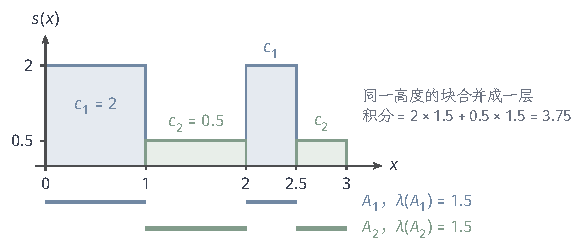
\includegraphics[width=98.771mm]{figures/02-abstract-mathematics/01-metric-and-measure/tikz/c3-simple-height-measure/figure.pdf}
 \caption{简单函数积分的“高度乘以测度”。$[0,3]$上的$s$在$A_1=[0,1)\cup[2,2.5)$（蓝）上取$2$，在$A_2=[1,2)\cup[2.5,3]$（绿）上取$0.5$；下方两行线段标出两层在横轴上占据的集合。积分为$2\times1.5+0.5\times1.5=3.75$。}
 \label{fig:integral-simple-height-measure}
\end{figure}

\paragraph{与表示方式无关}
同一个简单函数可以有多种写法，例如$\mathbf 1_{[0,2]}=1\cdot\mathbf 1_{[0,1]}+1\cdot\mathbf 1_{(1,2]}$，定义~\ref{def:integral-simple}允许任意一种不交写法，因此先要确认结果不依赖写法。办法是把两种写法放到共同的细分上比较。

\begin{lemma}[简单函数积分的良定性与基本运算]
\label{lem:integral-simple-properties}
设$s,t$是非负简单函数，$a\in[0,+\infty)$。
\begin{enumerate}
 \item $\int_Xs\,\mathrm d\mu$不依赖于$s$的不交表示。
 \item $\int_X(s+t)\,\mathrm d\mu=\int_Xs\,\mathrm d\mu+\int_Xt\,\mathrm d\mu$，$\int_Xas\,\mathrm d\mu=a\int_Xs\,\mathrm d\mu$。
 \item 若$s\le t$，则$\int_Xs\,\mathrm d\mu\le\int_Xt\,\mathrm d\mu$。
 \item 集合函数$E\mapsto\int_Es\,\mathrm d\mu$是$(X,\mathcal A)$上的测度。
\end{enumerate}
\end{lemma}

\begin{proof}
设$s=\sum_ic_i\mathbf 1_{A_i}=\sum_jd_j\mathbf 1_{B_j}$是两种不交表示。补上$A_0=X\setminus\bigcup_iA_i$与系数$c_0=0$，它贡献$0\cdot\mu(A_0)=0$，不改变定义中的和；对$B_j$同样处理。于是可设$\{A_i\}$与$\{B_j\}$都是$X$的有限可测分割。由有限可加性，$\mu(A_i)=\sum_j\mu(A_i\cap B_j)$，故
\[
 \sum_ic_i\mu(A_i)=\sum_{i,j}c_i\mu(A_i\cap B_j)=\sum_{i,j}d_j\mu(A_i\cap B_j)=\sum_jd_j\mu(B_j).
\]
中间一步逐项成立：若$A_i\cap B_j\ne\varnothing$，其中一点的函数值同时是$c_i$与$d_j$，故$c_i=d_j$；若交集为空，两边该项都为零。$[0,+\infty]$中有限非负数与和的分配律成立，所以上述运算不涉及无定义的表达式。第1条得证。

对第2条，取$s=\sum_ic_i\mathbf 1_{A_i}$、$t=\sum_jd_j\mathbf 1_{B_j}$为两个分割上的表示。在共同细分上，$s+t=\sum_{i,j}(c_i+d_j)\mathbf 1_{A_i\cap B_j}$是$s+t$的一个不交表示，由第1条
\[
 \int_X(s+t)\,\mathrm d\mu=\sum_{i,j}(c_i+d_j)\mu(A_i\cap B_j)=\int_Xs\,\mathrm d\mu+\int_Xt\,\mathrm d\mu.
\]
数乘只把每个系数乘以$a$。对第3条，在同一细分上，凡$A_i\cap B_j\ne\varnothing$就有$c_i\le d_j$，逐项比较$\sum_{i,j}c_i\mu(A_i\cap B_j)$与$\sum_{i,j}d_j\mu(A_i\cap B_j)$即得。

对第4条，$\int_Es\,\mathrm d\mu=\sum_ic_i\mu(A_i\cap E)$。每个$E\mapsto\mu(A_i\cap E)$都是测度：$E_n$两两不交时$A_i\cap E_n$也两两不交，可数可加性直接继承。有限个测度的非负系数组合仍是测度（引理~\ref{lem:measure-weighted-sum}），结论成立。
\end{proof}

第4条在区域之间比较累计值：$E\subseteq F$时$\int_Es\le\int_Fs$，递增区域上的累计值随区域收敛。下一小节以后的下方逼近要反复比较这样的累计值，第~\ref{sec:integral-mct}小节证明单调收敛定理时将用到它的从下连续性。

\subsection{简单函数逼近}
\label{sec:integral-simple-approximation}

\paragraph{按函数值分层}
一般可测函数在一块区域内可能不断改变取值，不能直接用有限个常值贡献精确累计。黎曼积分的做法是把定义域切成小区间，在每段上取一个代表值；这要求定义域是区间，也要求函数在小区间上变化不大。测度空间$X$上未必有“小区间”，可测函数也可能处处剧烈振荡。另一种做法是切分\emph{函数值}：把取值范围分成若干层，收集函数值落在同一层的全部点。这样的点集是阈值集合的差，对可测函数总是可测的，不论$X$是什么空间。图~\ref{fig:integral-riemann-lebesgue-partitions}对比了两种切法：同一层$\{f\ge1.5\}$在横轴上由两段不相邻的区间组成，测度只需把它们的长度相加。

\begin{figure}[!htbp]
 \centering
 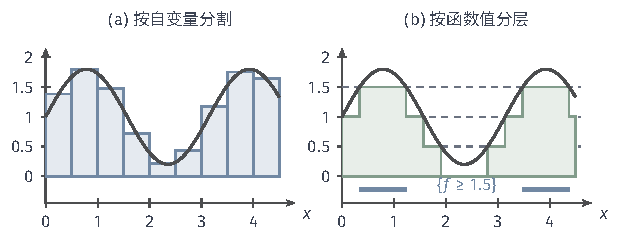
\includegraphics[width=104.881mm]{figures/02-abstract-mathematics/01-metric-and-measure/tikz/c3-riemann-lebesgue-partitions/figure.pdf}
 \caption{两种切分方式，$f(x)=1+0.8\sin2x$，$x\in[0,4.5]$。(a)把定义域等分为$9$段，每段取中点值作高度，这是黎曼和的做法。(b)把函数值按步长$0.5$分层，绿色阶梯是$0.5\lfloor2f\rfloor$；最高一层$\{f\ge1.5\}=[0.3376,1.2332)\cup[3.4792,4.3749)$（底部蓝色线段）由两段区间组成，总长约$1.79$。}
 \label{fig:integral-riemann-lebesgue-partitions}
\end{figure}

\begin{lemma}[简单函数逼近]
\label{lem:integral-simple-approx}
设$f:X\to[0,+\infty]$可测。令
\[
 s_n=2^{-n}\bigl\lfloor2^n\min\{f,n\}\bigr\rfloor,\qquad n=1,2,\dots.
\]
则每个$s_n$是非负简单函数，$0\le s_1\le s_2\le\cdots\le f$，且对每个$x\in X$有$s_n(x)\to f(x)$。若$f\le M$有界，则当$n\ge M$时$\sup_X(f-s_n)\le2^{-n}$，即$s_n$一致收敛到$f$。
\end{lemma}

\begin{proof}
\emph{$s_n$是简单函数。}若$f(x)\ge n$，则$\min\{f(x),n\}=n$，$s_n(x)=n$；若$f(x)<n$，则$s_n(x)=k2^{-n}$，其中$k=\lfloor2^nf(x)\rfloor\in\{0,1,\dots,n2^n-1\}$。所以
\[
 s_n=\sum_{k=0}^{n2^n-1}k2^{-n}\mathbf 1_{A_{n,k}}+n\mathbf 1_{\{f\ge n\}},\qquad A_{n,k}=\{k2^{-n}\le f<(k+1)2^{-n}\}.
\]
$A_{n,k}=\{f\ge k2^{-n}\}\setminus\{f\ge(k+1)2^{-n}\}$是两个阈值集合之差，可测；各集合两两不交，$s_n$只取有限多个值。

\emph{递增且不超过$f$。}由$\lfloor y\rfloor\le y$得$s_n\le\min\{f,n\}\le f$。对任意$y\ge0$，$2\lfloor y\rfloor$是不超过$2y$的整数，所以$2\lfloor y\rfloor\le\lfloor2y\rfloor$。记$m_n=\min\{f,n\}\le m_{n+1}$，则
\[
 s_n=2^{-(n+1)}\cdot2\lfloor2^nm_n\rfloor\le2^{-(n+1)}\lfloor2^{n+1}m_n\rfloor\le2^{-(n+1)}\lfloor2^{n+1}m_{n+1}\rfloor=s_{n+1}.
\]

\emph{逐点收敛。}若$f(x)=+\infty$，则$s_n(x)=n\to+\infty$。若$f(x)<+\infty$，当$n>f(x)$时$m_n(x)=f(x)$，由$\lfloor y\rfloor>y-1$得$0\le f(x)-s_n(x)<2^{-n}$。若$f\le M$，这个估计对$n\ge M$在全部$x$上同时成立：$n=M$而$f(x)=n$时差为零，其余情形差小于$2^{-n}$。
\end{proof}

图~\ref{fig:integral-dyadic-approximation}对$[0,2]$上的$f(x)=x^2$画出$s_1$与$s_2$。$n=1$时取值步长为$1/2$、高度截断于$1$，断点在$x=\sqrt{1/2}\approx0.7071$与$x=1$；$n=2$时步长缩为$1/4$、截断高度升到$2$，断点为$\sqrt{k/4}$，$k=1,\dots,8$。每增加一步，既把已有的层对半细分，又把截断线抬高一格，所以逼近从两个方向同时改进：细分处理函数值的细节，截断线的上升处理函数的大值。分层发生在函数值上，断点的位置由$f$决定，而不是事先在定义域上取定。

\begin{figure}[!htbp]
 \centering
 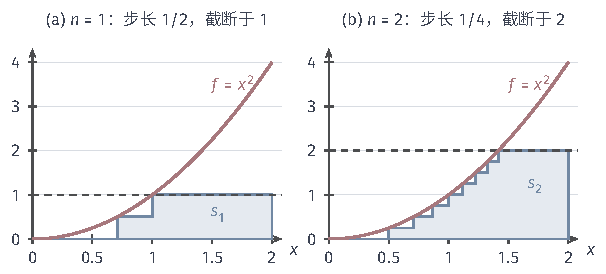
\includegraphics[width=102.634mm]{figures/02-abstract-mathematics/01-metric-and-measure/tikz/c3-dyadic-approximation/figure.pdf}
 \caption{二进分层逼近$f(x)=x^2$，$x\in[0,2]$。蓝色阶梯是$s_n=2^{-n}\lfloor2^n\min\{f,n\}\rfloor$，虚线是截断高度$n$。(a)$n=1$，$s_1$取值$0,0.5,1$；(b)$n=2$，$s_2$取值$0,0.25,\dots,2$，断点为$\sqrt{k/4}$。阶梯始终位于曲线下方，且随$n$增大而升高。}
 \label{fig:integral-dyadic-approximation}
\end{figure}

\paragraph{取正负值的函数}
可正可负的实值可测函数$f$不能直接套用上面的分层，因为下取整会把负值推得更负。把正值部分与负值部分分开处理即可。

\begin{definition}[正部与负部]
\label{def:integral-positive-negative-parts}
对可测函数$f:X\to[-\infty,+\infty]$，称$f^+=\max\{f,0\}$为$f$的\term{正部}（positive part），$f^-=\max\{-f,0\}$为$f$的\term{负部}（negative part）。
\end{definition}

由定理~\ref{thm:measure-function-operations}，$f^+$、$f^-$都是非负可测函数，且
\[
 f=f^+-f^-,\qquad |f|=f^++f^-.
\]
在每一点至多有一个部分非零：$f(x)>0$时$f^-(x)=0$，$f(x)<0$时$f^+(x)=0$。负部取的是$-f$的正值，所以它本身非负。图~\ref{fig:integral-positive-negative-parts}以$f=\sin x$为例：$f^+$在$[0,\pi]$上等于$\sin x$，$f^-$在$[\pi,2\pi]$上等于$-\sin x$，两者都画在横轴上方。

\begin{figure}[!htbp]
 \centering
 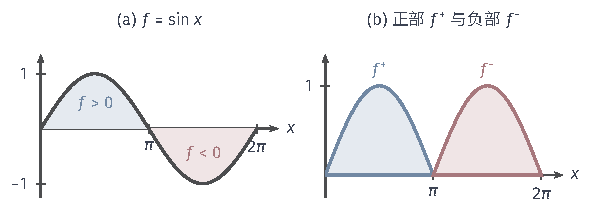
\includegraphics[width=100.034mm]{figures/02-abstract-mathematics/01-metric-and-measure/tikz/c3-positive-negative-parts/figure.pdf}
 \caption{正负部分解，$f(x)=\sin x$，$x\in[0,2\pi]$。(a)$f$在$[0,\pi]$上为正（蓝），在$[\pi,2\pi]$上为负（红）。(b)正部$f^+=\max\{f,0\}$与负部$f^-=\max\{-f,0\}$都是非负函数，且$f=f^+-f^-$，$|f|=f^++f^-$。}
 \label{fig:integral-positive-negative-parts}
\end{figure}

对实值可测$f$，分别用引理~\ref{lem:integral-simple-approx}构造$s_n^+\uparrow f^+$与$s_n^-\uparrow f^-$，令$\varphi_n=s_n^+-s_n^-$。它是简单函数，逐点收敛到$f$，并且$|\varphi_n|\le s_n^++s_n^-\le|f|$，即逼近函数始终受$|f|$控制。若$|f|\le M$，因为每点只有一个部分起作用，$n\ge M$时$\sup_X|f-\varphi_n|\le2^{-n}$，逼近是一致的。至此一般可测函数与简单函数之间的逼近关系已经建立；这些逼近函数的积分是否收敛到某个确定的数，要在定义积分以后才能讨论。

\subsection{非负可测函数的积分}
\label{sec:integral-nonnegative}

\paragraph{下方逼近的上确界}
对非负可测函数$f$，位于$f$下方的每个非负简单函数$s$都给出总贡献的一个偏小估计$\int s\,\mathrm d\mu$。上一小节说明这样的$s$能够逐层读出$f$的取值，所以把全部偏小估计的上确界作为积分是合理的。定义并不指定使用哪一条逼近列，这避免了“换一列逼近是否得到同一个数”的问题。

\begin{definition}[非负可测函数的积分]
\label{def:integral-nonnegative}
设$f:X\to[0,+\infty]$可测。定义
\[
 \int_Xf\,\mathrm d\mu=\sup\Bigl\{\int_Xs\,\mathrm d\mu:\ s\text{是非负简单函数},\ 0\le s\le f\Bigr\}\in[0,+\infty].
\]
对$E\in\mathcal A$，令$\int_Ef\,\mathrm d\mu=\int_Xf\mathbf 1_E\,\mathrm d\mu$。这样得到的积分称为$f$关于$\mu$的\term{Lebesgue积分}（Lebesgue integral）。在实轴上对Lebesgue测度积分时，也写作$\int_Ef(x)\,\mathrm dx$。
\end{definition}

若$f$本身是非负简单函数，它是候选集合中的一员；由引理~\ref{lem:integral-simple-properties}第3条，其余候选的积分都不超过$\int f$，所以上确界恰好是定义~\ref{def:integral-simple}的值，两个定义一致。沿某一条递增逼近列取极限也得到这个上确界，这一点要用到第~\ref{sec:integral-mct}小节的单调收敛定理。

\begin{example}[直接由定义计算$\int_{[0,1]}x\,\mathrm dx$]
\label{ex:integral-identity-on-unit}
在$[0,1]$上取$f(x)=x$。把$[0,1]$分成$2^n$段$I_k=[k2^{-n},(k+1)2^{-n})$，$k=0,\dots,2^n-2$，最后一段取闭区间$I_{2^n-1}=[1-2^{-n},1]$。令
\[
 s_n=\sum_{k=0}^{2^n-1}k2^{-n}\mathbf 1_{I_k},\qquad t_n=\sum_{k=0}^{2^n-1}(k+1)2^{-n}\mathbf 1_{I_k},
\]
则$s_n\le f\le t_n$在$[0,1]$上处处成立。$s_n$是候选之一，故$\int_{[0,1]}f\ge\int s_n=\sum_k k2^{-2n}=\tfrac12(1-2^{-n})$。另一方面，任一候选$s\le f\le t_n$满足$\int s\le\int t_n=\sum_k(k+1)2^{-2n}=\tfrac12(1+2^{-n})$，所以上确界也不超过此数。令$n\to\infty$，得$\int_{[0,1]}x\,\mathrm dx=\tfrac12$。
\end{example}

这个例子只用了定义和简单函数的单调性：下方的简单函数给出下界，上方的简单函数控制全部候选，从而给出上界。对大多数函数，这样直接夹逼并不方便；第~\ref{sec:integral-classical}节将证明黎曼可积函数的Lebesgue积分就是原来的黎曼积分，届时可以用原函数计算。

\paragraph{单调性与零测集}
积分对函数的比较和对零测集的忽略，都可以直接从定义读出。

\begin{lemma}[非负积分的基本性质]
\label{lem:integral-nonnegative-basic}
设$f,g:X\to[0,+\infty]$可测。
\begin{enumerate}
 \item 若$f\le g$，则$\int_Xf\,\mathrm d\mu\le\int_Xg\,\mathrm d\mu$。
 \item 对$a\in(0,+\infty)$，$a\,\mu(\{f\ge a\})\le\int_Xf\,\mathrm d\mu$。
 \item 若$f=g$ $\mu$-几乎处处，则$\int_Xf\,\mathrm d\mu=\int_Xg\,\mathrm d\mu$；特别地，对零测集$N$有$\int_Nf\,\mathrm d\mu=0$。
 \item $\int_Xf\,\mathrm d\mu=0$当且仅当$f=0$ $\mu$-几乎处处。
 \item 若$\int_Xf\,\mathrm d\mu<+\infty$，则$\mu(\{f=+\infty\})=0$。
\end{enumerate}
\end{lemma}

\begin{proof}
第1条：$f\le g$时，$f$下方的候选简单函数都在$g$下方，上确界取自更大的集合。第2条：$a\mathbf 1_{\{f\ge a\}}$是$f$下方的简单函数，其积分为$a\mu(\{f\ge a\})$。

第3条：按定义~\ref{def:measure-null-set}，存在零测集$N\in\mathcal A$，使$f=g$在$N$外成立。设$s=\sum_ic_i\mathbf 1_{A_i}\le f$是候选简单函数。在$N$外$s\le f=g$，在$N$上$s\mathbf 1_{X\setminus N}=0$，所以$s\mathbf 1_{X\setminus N}\le g$。又$\int s\mathbf 1_N=\sum_ic_i\mu(A_i\cap N)=0$，由引理~\ref{lem:integral-simple-properties}第2条，
\[
 \int_Xs\,\mathrm d\mu=\int_Xs\mathbf 1_{X\setminus N}\,\mathrm d\mu+\int_Xs\mathbf 1_N\,\mathrm d\mu=\int_Xs\mathbf 1_{X\setminus N}\,\mathrm d\mu\le\int_Xg\,\mathrm d\mu.
\]
对$s$取上确界得$\int f\le\int g$，交换$f,g$得等式。取$g=0$并把$f$换成$f\mathbf 1_N$，得$\int_Nf=0$。

第4条：若$f=0$几乎处处，由第3条$\int f=\int0=0$。反之设$\int f=0$。由第2条，$\mu(\{f\ge1/n\})\le n\int f=0$；而$\{f>0\}=\bigcup_n\{f\ge1/n\}$，由可数次可加性它是零测集。第5条：对每个$M>0$，$\{f=+\infty\}\subseteq\{f\ge M\}$，由第2条$\mu(\{f=+\infty\})\le\frac1M\int f$，令$M\to+\infty$即得。
\end{proof}

第3条说明积分忽略零测集上的改动。例如在$[0,1]$上令$f=\mathbf 1_{[0,1]}+\infty\cdot\mathbf 1_{\mathbb Q\cap[0,1]}$，它在可数个点上取$+\infty$，但这些点组成零测集，所以$\int_{[0,1]}f\,\mathrm d\lambda=\int_{[0,1]}1\,\mathrm d\lambda=1$。第2条把集合的测度与函数的积分联系起来，第4、5两条则从“积分为零”或“积分有限”反推函数在几乎所有点上的行为，后面证明收敛定理时会反复用到。

使用第3条时要注意可测性。引理假定$f$与$g$都可测；若只知道$g$与可测的$f$在零测集外相等，$g$是否可测取决于测度空间是否完备（定义~\ref{def:measure-complete}）。Lebesgue测度空间$(\mathbb R,\mathcal L,\lambda)$是完备的，任意修改零测集上的值都保持可测；在$(\mathbb R,\mathcal B(\mathbb R),\lambda)$上则需要另行确认修改后的函数Borel可测。

\subsection{实值与复值函数的积分}
\label{sec:integral-real-complex}

\paragraph{正负贡献分别累计}
被积函数可以取负值时，先把正贡献与负贡献分别累计，再相减。只要两个累计值不同时为$+\infty$，差就有确定的意义；要让结果成为有限实数，则需要两者都有限。

\begin{definition}[积分存在与Lebesgue可积]
\label{def:integral-integrable}
设$f:X\to[-\infty,+\infty]$可测。
\begin{enumerate}
 \item 若$\int_Xf^+\,\mathrm d\mu$与$\int_Xf^-\,\mathrm d\mu$至少一个有限，称$f$的积分存在，并定义
 \[
  \int_Xf\,\mathrm d\mu=\int_Xf^+\,\mathrm d\mu-\int_Xf^-\,\mathrm d\mu\in[-\infty,+\infty].
 \]
 \item 若$\int_X|f|\,\mathrm d\mu<+\infty$，称$f$关于$\mu$\term{Lebesgue可积}（Lebesgue integrable），简称$\mu$-可积。
 \item 设$f=u+\mathrm iv$是复值函数，$u,v$为实值可测函数。若$\int_X|f|\,\mathrm d\mu<+\infty$，称$f$为$\mu$-可积，并定义$\int_Xf\,\mathrm d\mu=\int_Xu\,\mathrm d\mu+\mathrm i\int_Xv\,\mathrm d\mu$。
\end{enumerate}
全体$\mu$-可积函数（按上下文取实值或复值）记作$L^1(\mu)$。对$E\in\mathcal A$，仍以$\int_Ef\,\mathrm d\mu=\int_Xf\mathbf 1_E\,\mathrm d\mu$定义区域上的积分。
\end{definition}

可积时两部分都有限，因为$f^+\le|f|$、$f^-\le|f|$，由引理~\ref{lem:integral-nonnegative-basic}第1条，$\int f^\pm\le\int|f|<+\infty$。于是积分是一个有限实数，并由引理~\ref{lem:integral-nonnegative-basic}第5条，可积函数几乎处处取有限值。反过来，两部分都有限能否推出$\int|f|$有限，要用到非负积分的加法$\int|f|=\int f^++\int f^-$，留到第~\ref{sec:integral-signed-rules}小节证明。

三种情形需要分开。在$(\mathbb R,\lambda)$上，$f=2\cdot\mathbf 1_{[0,1)}-\mathbf 1_{[1,3)}$满足$\int f^+=2$、$\int f^-=2$，可积，积分为$0$。$g=\mathbf 1_{[0,1]}-\mathbf 1_{(1,+\infty)}$满足$\int g^+=1$、$\int g^-=+\infty$，积分存在且等于$-\infty$，但$g$不可积。$h=\mathbf 1_{[0,+\infty)}-\mathbf 1_{(-\infty,0)}$的两部分积分都是$+\infty$，差$+\infty-(+\infty)$没有定义，$h$的积分不存在。允许单侧无穷的积分在比较大小时有用，但本章的运算规则主要针对可积函数。

\paragraph{复值函数}
对复值函数，$|f|=\sqrt{u^2+v^2}$由$u,v$经连续运算得到，可测。因为$|u|\le|f|$、$|v|\le|f|$，复值可积函数的实部与虚部都是实值可积函数，定义中的两个积分都是有限实数。例如在$[0,2]$上取$f=\mathrm i\,\mathbf 1_{[0,1]}+(1-\mathrm i)\mathbf 1_{(1,2]}$，则$\int|f|\,\mathrm d\lambda=1+\sqrt2$，$f$可积；实部为$\mathbf 1_{(1,2]}$，虚部为$\mathbf 1_{[0,1]}-\mathbf 1_{(1,2]}$，所以$\int f\,\mathrm d\lambda=1+\mathrm i(1-1)=1$。第~\ref{sec:integral-signed-rules}小节还将证明，复值$f$可积当且仅当实部与虚部分别可积。

这里改变的是被积函数的取值范围，测度始终非负。下一小节改变测度的取值范围：测度本身可以给集合赋负值，这时“正”和“负”来自集合上的质量，而不是来自函数值。

\subsection{有符号测度的积分}
\label{sec:integral-signed-measure}

\paragraph{分别对正负质量积分}
第~\ref{sec:measure-signed}节的有限有符号测度$\eta$有唯一的Jordan分解$\eta=\eta^+-\eta^-$（定理~\ref{thm:measure-jordan}），总变差测度为$|\eta|=\eta^++\eta^-$（定义~\ref{def:measure-total-variation}）。$\eta^+$、$\eta^-$都是非负测度，前面的积分对它们已有定义，所以可以先分别累计，再相减。为使相减有意义，要求函数对总变差绝对可积，这同时控制了对两部分的积分。

\begin{lemma}[非负积分对测度的单调性]
\label{lem:integral-measure-monotone}
设$\nu,\rho$是$(X,\mathcal A)$上的测度，且$\nu(A)\le\rho(A)$对一切$A\in\mathcal A$成立。则对非负可测$g$，$\int_Xg\,\mathrm d\nu\le\int_Xg\,\mathrm d\rho$。
\end{lemma}

\begin{proof}
对非负简单函数$s=\sum_ic_i\mathbf 1_{A_i}$，$\int s\,\mathrm d\nu=\sum_ic_i\nu(A_i)\le\sum_ic_i\rho(A_i)=\int s\,\mathrm d\rho$。对$g$下方的全部简单函数取上确界即得。
\end{proof}

由$\eta^\pm(A)\le\eta^+(A)+\eta^-(A)=|\eta|(A)$，若$\int|f|\,\mathrm d|\eta|<+\infty$，则$\int|f|\,\mathrm d\eta^+$与$\int|f|\,\mathrm d\eta^-$都有限，$f$对$\eta^+$、$\eta^-$都可积。

\begin{definition}[有符号测度的积分]
\label{def:integral-signed-measure}
设$\eta$是$(X,\mathcal A)$上的有限有符号测度，$f$是实值或复值可测函数，且$\int_X|f|\,\mathrm d|\eta|<+\infty$。定义
\[
 \int_Xf\,\mathrm d\eta=\int_Xf\,\mathrm d\eta^+-\int_Xf\,\mathrm d\eta^-.
\]
\end{definition}

右端只依赖测度$\eta^+,\eta^-$，而Jordan分解是唯一的：Hahn分解中正、负区域可以有不同的选取，但限制在其上得到的$\eta^\pm$相同。因此定义只依赖$\eta$本身。取$f=\mathbf 1_A$得$\int\mathbf 1_A\,\mathrm d\eta=\eta^+(A)-\eta^-(A)=\eta(A)$，与集合上的赋值一致。这一定义只调用了第~\ref{chap:measures}章的分解与本节已有的积分，不需要先证明一般积分的线性性。

\begin{example}[有限点集上的正负质量]
\label{ex:integral-signed-measure-points}
在$X=\{a,b,c\}$（全部子集可测）上取$\eta=2\delta_a-3\delta_b+\delta_c$，函数$f(a)=1$、$f(b)=2$、$f(c)=-4$。Jordan分解为$\eta^+=2\delta_a+\delta_c$、$\eta^-=3\delta_b$，$|\eta|=2\delta_a+3\delta_b+\delta_c$。$f$在有限集上只取有限个值，各部分都是简单函数，直接计算得
\[
 \begin{aligned}
  \int f\,\mathrm d\eta^+&=2\cdot1+1\cdot(-4)=-2,\\
  \int f\,\mathrm d\eta^-&=3\cdot2=6,\\
  \int f\,\mathrm d\eta&=-8.
 \end{aligned}
\]
它等于逐点贡献之和$f(a)\eta(\{a\})+f(b)\eta(\{b\})+f(c)\eta(\{c\})=2-6-4$。绝对贡献为$\int|f|\,\mathrm d|\eta|=2+6+4=12$。
\end{example}

图~\ref{fig:integral-signed-measure-masses}把这个计算画成质量柱与贡献表。负的贡献有两种来源：点$b$上函数值为正而质量为负，点$c$上质量为正而函数值为负。前者来自测度的符号，后者来自函数的符号，两种正负分别由Jordan分解与上一小节的正负部处理。可积条件只要求绝对贡献的总和有限；关于有符号测度积分的线性规则与估计$|\int f\,\mathrm d\eta|\le\int|f|\,\mathrm d|\eta|$，在第~\ref{sec:integral-signed-measure-rules}小节证明。

\begin{figure}[!htbp]
 \centering
 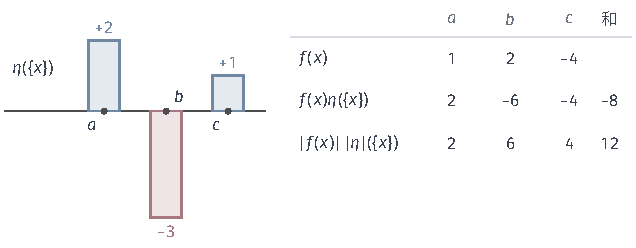
\includegraphics[width=107.692mm]{figures/02-abstract-mathematics/01-metric-and-measure/tikz/c3-signed-measure-masses/figure.pdf}
 \caption{有符号测度$\eta=2\delta_a-3\delta_b+\delta_c$上的积分。左侧柱高为各点质量$\eta(\{x\})$，蓝色为正、红色为负；右表列出$f$的取值、逐点贡献$f(x)\eta(\{x\})$及其和$-8$，以及绝对贡献$|f(x)|\,|\eta|(\{x\})$及其和$12$。}
 \label{fig:integral-signed-measure-masses}
\end{figure}

\section{积分的基本性质}
\label{sec:integral-properties}

上一节的积分由上确界定义，单调性可以直接读出，但加法却不明显：$f$下方的简单函数与$g$下方的简单函数相加，得到的只是$f+g$下方的一部分候选，不能立即推出$\int(f+g)=\int f+\int g$。本节先证明非负函数的递增逼近可以与积分交换，借此把简单函数的运算规则传递到一般非负函数；随后分别处理可正可负的实值函数与复值函数，最后把这些规则推广到上一节已经定义的有符号测度积分。

\subsection{单调收敛定理}
\label{sec:integral-mct}

\paragraph{定理与证明}
定义~\ref{def:integral-nonnegative}没有指定逼近列。若一列非负函数从下方递增地逼近$f$，它们的积分是否趋于$\int f$？下面的定理给出肯定回答，并允许两边同时为$+\infty$。

\begin{theorem}[单调收敛定理]
\label{thm:integral-monotone-convergence}
设$f_1,f_2,\dots:X\to[0,+\infty]$可测，且$f_1\le f_2\le\cdots$处处成立，令$f=\lim_nf_n=\sup_nf_n$。则$f$可测，并且
\[
 \lim_{n\to\infty}\int_Xf_n\,\mathrm d\mu=\int_Xf\,\mathrm d\mu,
\]
两边可以同时等于$+\infty$。这一结论称为\term{单调收敛定理}（monotone convergence theorem）。
\end{theorem}

\begin{proof}
$f$是可数个可测函数的上确界，由定理~\ref{thm:measure-limits}可测。由引理~\ref{lem:integral-nonnegative-basic}第1条，$\int f_n$关于$n$递增，且每项不超过$\int f$；记极限为$L\in[0,+\infty]$，则$L\le\int f$。

反向不等式需要说明$f$下方的每个简单函数都被$f_n$的积分最终超过。固定非负简单函数$s\le f$与常数$c\in(0,1)$，令
\[
 E_n=\{x:f_n(x)\ge c\,s(x)\}.
\]
把$s$写成分割上的表示$s=\sum_ic_i\mathbf 1_{A_i}$，则$E_n=\bigcup_i\bigl(A_i\cap\{f_n\ge cc_i\}\bigr)$是阈值集合与可测集之交的有限并，可测；并且由$f_n$递增知$E_1\subseteq E_2\subseteq\cdots$。这列集合填满$X$：若$s(x)=0$，则$x\in E_1$；若$s(x)>0$，则$cs(x)<s(x)\le f(x)=\sup_nf_n(x)$，故某个$f_n(x)\ge cs(x)$。在$E_n$上$f_n\ge cs$，因此
\[
 \int_Xf_n\,\mathrm d\mu\ge\int_Xf_n\mathbf 1_{E_n}\,\mathrm d\mu\ge c\int_{E_n}s\,\mathrm d\mu.
\]

由引理~\ref{lem:integral-simple-properties}第4条，$E\mapsto\int_Es\,\mathrm d\mu$是测度；由测度的从下连续性（定理~\ref{thm:measure-basic-properties}），$\int_{E_n}s\to\int_Xs$。令$n\to\infty$得$L\ge c\int_Xs$。再令$c\uparrow1$得$L\ge\int s$，对$f$下方的全部$s$取上确界，得$L\ge\int f$。
\end{proof}

缩小因子$c<1$是证明的关键。若直接取$E_n=\{f_n\ge s\}$，在$f(x)=s(x)$而每个$f_n(x)<f(x)$的点上，$x$永远不进入$E_n$，集合列就不能填满$X$。乘以$c$留出一点余量，使严格不等式$cs(x)<f(x)$能被递增列在有限步内越过。图~\ref{fig:integral-monotone-convergence-sets}在$[0,1]$上取$f_n(x)=x^{1/n}$，它递增到$f=\mathbf 1_{(0,1]}$；取$s=0.8\cdot\mathbf 1_{(0,1]}$、$c=0.9$，集合$E_n=[0.72^n,1]$随$n$向左扩张，左端点依次为$0.72$、$0.5184$、$0.2687$（$n=1,2,4$），最终覆盖$(0,1]$。

\begin{figure}[!htbp]
 \centering
 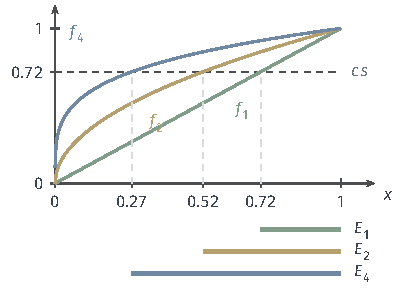
\includegraphics[width=68.273mm]{figures/02-abstract-mathematics/01-metric-and-measure/tikz/c3-monotone-convergence-sets/figure.pdf}
 \caption{单调收敛定理证明中的集合$E_n=\{f_n\ge cs\}$。$f_n(x)=x^{1/n}$（$n=1,2,4$）在$[0,1]$上递增到$\mathbf 1_{(0,1]}$；取$s=0.8\cdot\mathbf 1_{(0,1]}$、$c=0.9$，虚线为高度$cs=0.72$。下方三条线段是$E_n=[0.72^n,1]$，它们递增并逐步覆盖$(0,1]$。}
 \label{fig:integral-monotone-convergence-sets}
\end{figure}

定理只要求逐点递增与非负，不要求$f_n$或$f$可积。若递增与收敛只在零测集外成立，把各个零测例外合并为一个零测集$N$（可数个零测集之并仍为零测集），在$N$外应用定理于$f_n\mathbf 1_{X\setminus N}$，再由引理~\ref{lem:integral-nonnegative-basic}第3条知积分不受影响；这里需要$f$本身可测，在完备空间上这一点自动成立。

\paragraph{与简单函数逼近的衔接}
把定理用于引理~\ref{lem:integral-simple-approx}构造的$s_n\uparrow f$，立即得到
\[
 \int_Xf\,\mathrm d\mu=\lim_{n\to\infty}\int_Xs_n\,\mathrm d\mu.
\]
任何从下方递增逼近$f$的简单函数列都给出同一个极限，它就是定义中的上确界。这一结论使简单函数的有限运算能够传递到一般非负函数，下一小节正是这样做的。单调收敛定理在逐项求和、递增区域等计算中的使用，集中在第~\ref{sec:integral-limits-monotone}小节，后文不再重复证明。

\subsection{非负积分的运算性质}
\label{sec:integral-nonnegative-rules}

\paragraph{加法与数乘}
有了单调收敛定理，加法只需在逼近列上验证。

\begin{theorem}[非负积分的线性]
\label{thm:integral-nonnegative-linear}
设$f,g:X\to[0,+\infty]$可测，$a,b\in[0,+\infty)$。则
\[
 \int_X(af+bg)\,\mathrm d\mu=a\int_Xf\,\mathrm d\mu+b\int_Xg\,\mathrm d\mu.
\]
\end{theorem}

\begin{proof}
取引理~\ref{lem:integral-simple-approx}中的简单函数$s_n\uparrow f$、$t_n\uparrow g$。则$as_n+bt_n$是非负简单函数，逐点递增到$af+bg$（在$f$或$g$取$+\infty$的点上，按$[0,+\infty]$中的运算理解，且$0\cdot(+\infty)=0$）。由引理~\ref{lem:integral-simple-properties}第2条，$\int(as_n+bt_n)=a\int s_n+b\int t_n$。对两边令$n\to\infty$，三次应用单调收敛定理即得。
\end{proof}

这里只累计非负贡献，所有和都在$[0,+\infty]$中进行，不会出现无穷相减；当$a=0$而$\int f=+\infty$时，约定$0\cdot(+\infty)=0$与$af=0$的积分为零相符。例如在$[0,1]$上，由例~\ref{ex:integral-identity-on-unit}与$\int_{[0,1]}1\,\mathrm d\lambda=1$，得$\int_{[0,1]}(x+3)\,\mathrm dx=\tfrac12+3=\tfrac72$。

\paragraph{比较、区域与上下界}
单调性（引理~\ref{lem:integral-nonnegative-basic}第1条）与加法结合，就得到区域积分的常用规则。若$E,F\in\mathcal A$不交，则$f\mathbf 1_{E\cup F}=f\mathbf 1_E+f\mathbf 1_F$，由加法
\[
 \int_{E\cup F}f\,\mathrm d\mu=\int_Ef\,\mathrm d\mu+\int_Ff\,\mathrm d\mu,
\]
对有限个两两不交的区域同样成立。若$E\subseteq F$，则$f\mathbf 1_E\le f\mathbf 1_F$，故$\int_Ef\le\int_Ff$。若在$E$上$m\le f\le M$，则$m\mathbf 1_E\le f\mathbf 1_E\le M\mathbf 1_E$，得到上下界
\[
 m\,\mu(E)\le\int_Ef\,\mathrm d\mu\le M\,\mu(E).
\]

这些规则把分段给出的函数拆开计算。在$[0,2]$上令$f(x)=x$（$0\le x\le1$）、$f(x)=1$（$1<x\le2$），则$\int_{[0,2]}f=\int_{[0,1]}x\,\mathrm dx+\int_{(1,2]}1\,\mathrm dx=\tfrac12+1=\tfrac32$。又因为$0\le f\le1$，上下界给出$0\le\int_{[0,2]}f\le2$，与计算结果相容。对可数个不交区域的累计，需要交换积分与无限求和，第~\ref{sec:integral-limits-monotone}小节再用单调收敛定理处理。

\subsection{有符号积分的运算性质}
\label{sec:integral-signed-rules}

本小节的“有符号”指被积函数可正可负，测度本身仍然非负；复值情形沿用把函数拆成分量的办法。

\paragraph{可积性与线性}
先补全可积性的两个等价说法。对实值可测$f$，由定理~\ref{thm:integral-nonnegative-linear}，
\[
 \int_X|f|\,\mathrm d\mu=\int_Xf^+\,\mathrm d\mu+\int_Xf^-\,\mathrm d\mu,
\]
所以$f$可积当且仅当$\int f^+$与$\int f^-$都有限。对复值$f=u+\mathrm iv$，由$|f|\le|u|+|v|$与$|u|,|v|\le|f|$，并由单调性和加法，$f$可积当且仅当$u$与$v$都可积。可积的扩展实值函数几乎处处有限（引理~\ref{lem:integral-nonnegative-basic}第5条），把它在取无穷值的零测集上改为$0$不改变任何积分，因此下面只讨论取有限值的函数。

\begin{theorem}[积分的线性]
\label{thm:integral-linear}
设$f,g\in L^1(\mu)$为实值（或复值）函数，$a,b$为实数（或复数）。则$af+bg\in L^1(\mu)$，并且
\[
 \int_X(af+bg)\,\mathrm d\mu=a\int_Xf\,\mathrm d\mu+b\int_Xg\,\mathrm d\mu.
\]
\end{theorem}

\begin{proof}
可积性：$|af+bg|\le|a||f|+|b||g|$，由单调性与非负积分的线性，$\int|af+bg|\le|a|\int|f|+|b|\int|g|<+\infty$。

实值情形的加法。令$h=f+g$，则$h^+-h^-=f^+-f^-+g^+-g^-$，移项得
\[
 h^++f^-+g^-=h^-+f^++g^+.
\]
两边都是非负可测函数之和，由定理~\ref{thm:integral-nonnegative-linear}，$\int h^++\int f^-+\int g^-=\int h^-+\int f^++\int g^+$。六个积分都是有限数，移项即得$\int h=\int f+\int g$。

实值情形的数乘。若$a\ge0$，则$(af)^\pm=af^\pm$，由非负积分的数乘得$\int af=a\int f$；若$a<0$，则$(af)^+=|a|f^-$、$(af)^-=|a|f^+$，故$\int af=|a|\int f^--|a|\int f^+=a\int f$。

复值情形。设$f=u+\mathrm iv$，$a=\alpha+\mathrm i\beta$，则$af=(\alpha u-\beta v)+\mathrm i(\alpha v+\beta u)$。按定义与实值线性，
\[
 \begin{aligned}
  \int af&=\Bigl(\alpha\int u-\beta\int v\Bigr)+\mathrm i\Bigl(\alpha\int v+\beta\int u\Bigr)\\
  &=(\alpha+\mathrm i\beta)\Bigl(\int u+\mathrm i\int v\Bigr)=a\int f.
 \end{aligned}
\]
复值的加法逐个分量使用实值加法即可。
\end{proof}

线性也给出可积实值函数之间的比较：若$f\le g$且两者可积，则$g-f\ge0$，$\int g-\int f=\int(g-f)\ge0$。

\paragraph{绝对值估计}
积分的大小受绝对贡献的总量控制。实值函数可以利用大小比较，复值函数则需要先把积分结果旋转到实轴上。

\begin{theorem}[积分的绝对值估计]
\label{thm:integral-abs-bound}
对实值或复值$f\in L^1(\mu)$，有$\bigl|\int_Xf\,\mathrm d\mu\bigr|\le\int_X|f|\,\mathrm d\mu$。
\end{theorem}

\begin{proof}
实值情形：$-|f|\le f\le|f|$，由上面的比较得$-\int|f|\le\int f\le\int|f|$。复值情形：记$z=\int f$，若$z=0$无须证明。否则令$\alpha=\overline z/|z|$，则$|\alpha|=1$且$\alpha z=|z|$。由线性，$\int\alpha f=\alpha z=|z|$是实数，所以它等于实部的积分$\int\operatorname{Re}(\alpha f)$。由$\operatorname{Re}(\alpha f)\le|\alpha f|=|f|$与实值比较，$|z|=\int\operatorname{Re}(\alpha f)\le\int|f|$。
\end{proof}

估计中的等号对实值函数在$f$几乎处处不变号时成立，一般则严格：$f=\mathbf 1_{[0,1)}-\mathbf 1_{[1,2)}$在$[0,2]$上积分为$0$，而$\int|f|=2$。实值函数可以比较大小，复值函数没有大小顺序，只能使用这类模长估计。

\paragraph{用可积函数控制}
判断可积性时，往往不必计算$\int|f|$，只需找一个已知可积的上界。若$f$可测、$g\ge0$可积且$|f|\le g$几乎处处成立，则由引理~\ref{lem:integral-nonnegative-basic}第1、3条，$\int|f|\le\int g<+\infty$，$f$可积。特别地，在有限测度空间上，若$|f|\le M$，取$g=M$得$\int|f|\le M\mu(X)$：有界可测函数都可积。例如$f(x)=\sin(1/x)$在$(0,1]$上连续，因而Borel可测，又$|f|\le1$、$\lambda((0,1])=1$，所以它对$\lambda$可积，并且$\bigl|\int_{(0,1]}f\,\mathrm d\lambda\bigr|\le1$。这里不需要$f$在$0$附近有极限。

上面的规则都针对有限积分。对只是积分存在、可能取$\pm\infty$的实值函数，必须逐次检查表达式是否出现无定义的$\infty-\infty$，不能照搬线性。在$(\mathbb R,\lambda)$上取$f=\mathbf 1_{[0,+\infty)}$与$g=-\mathbf 1_{[0,+\infty)}$，两者的积分分别存在且等于$+\infty$与$-\infty$；$f+g=0$的积分是$0$，而$\int f+\int g=+\infty-\infty$没有意义。

\subsection{有符号测度积分的运算性质}
\label{sec:integral-signed-measure-rules}

\paragraph{测度相加时的积分}
第~\ref{sec:integral-signed-measure}小节把有符号测度的积分写成对Jordan正负部分的两个积分之差。要估计它的大小，需要知道对$|\eta|=\eta^++\eta^-$的积分怎样拆开。

\begin{lemma}[测度之和的积分]
\label{lem:integral-sum-of-measures}
设$\nu,\rho$是$(X,\mathcal A)$上的测度，$g\ge0$可测。则$\int_Xg\,\mathrm d(\nu+\rho)=\int_Xg\,\mathrm d\nu+\int_Xg\,\mathrm d\rho$。若$f$对$\nu+\rho$可积，则它对$\nu,\rho$都可积，上式对$f$也成立。
\end{lemma}

\begin{proof}
对非负简单函数$s=\sum_ic_i\mathbf 1_{A_i}$，$\int s\,\mathrm d(\nu+\rho)=\sum_ic_i(\nu(A_i)+\rho(A_i))=\int s\,\mathrm d\nu+\int s\,\mathrm d\rho$。取$s_n\uparrow g$，对三个测度分别应用单调收敛定理，得到非负情形。若$f$对$\nu+\rho$可积，由非负情形$\int|f|\,\mathrm d\nu\le\int|f|\,\mathrm d(\nu+\rho)<+\infty$，对$\rho$同理；把$f$拆成正负部（复值时再拆实部与虚部），逐项应用非负情形并相减。
\end{proof}

\begin{theorem}[有符号测度积分的运算规则]
\label{thm:integral-signed-measure-rules}
设$\eta$是有限有符号测度，$f,g$为实值或复值可测函数，且$\int|f|\,\mathrm d|\eta|$、$\int|g|\,\mathrm d|\eta|$有限。
\begin{enumerate}
 \item 对实数（或复数）$a,b$，$af+bg$满足同样的可积条件，且$\int(af+bg)\,\mathrm d\eta=a\int f\,\mathrm d\eta+b\int g\,\mathrm d\eta$。
 \item $\bigl|\int_Xf\,\mathrm d\eta\bigr|\le\int_X|f|\,\mathrm d|\eta|$。
\end{enumerate}
\end{theorem}

\begin{proof}
第1条：$|af+bg|\le|a||f|+|b||g|$，故$af+bg$对$|\eta|$可积，从而对$\eta^\pm$可积（第~\ref{sec:integral-signed-measure}小节）。对$\eta^+$与$\eta^-$分别使用定理~\ref{thm:integral-linear}，两式相减即得。

第2条：由定理~\ref{thm:integral-abs-bound}与引理~\ref{lem:integral-sum-of-measures}，
\[
 \begin{aligned}
  \Bigl|\int f\,\mathrm d\eta\Bigr|
  &\le\Bigl|\int f\,\mathrm d\eta^+\Bigr|+\Bigl|\int f\,\mathrm d\eta^-\Bigr|\\
  &\le\int|f|\,\mathrm d\eta^++\int|f|\,\mathrm d\eta^-=\int|f|\,\mathrm d|\eta|.
 \end{aligned}
\]
\end{proof}

估计可以取到等号。设$(P,N)$是$\eta$的Hahn分解（定理~\ref{thm:measure-hahn}），令$f=\mathbf 1_P-\mathbf 1_N$。由$\eta^+(N)=0$、$\eta^-(P)=0$，$\int f\,\mathrm d\eta=\eta^+(P)+\eta^-(N)=|\eta|(X)$，而$|f|=1$，右端也是$|\eta|(X)$。例~\ref{ex:integral-signed-measure-points}中$|-8|<12$，原因是$f$的符号没有与质量的符号配合：点$c$上质量为正而函数值为负。

\paragraph{保序性不再成立}
总变差控制累计的绝对贡献，但有符号测度积分没有一般的保序性。在$X=\{a,b\}$（$a\ne b$）上取$\eta=\delta_a-\delta_b$，则$0\le\mathbf 1_{\{b\}}$，而$\int\mathbf 1_{\{b\}}\,\mathrm d\eta=\eta(\{b\})=-1<0=\int0\,\mathrm d\eta$。非负测度的单调性来自“每块质量非负”；质量可以为负时，增大函数值反而可能减小积分。因此对有符号测度只能使用线性规则与总变差估计，比较大小时需要回到$\eta^+$与$\eta^-$分别处理。

\section{与经典积分的关系}
\label{sec:integral-classical}

一般积分已经有了定义和运算规则，现在把它与此前熟悉的累计方式逐一对应。离散求和对每个点按权重累加；闭区间上的黎曼积分用分割与上下和夹逼；反常积分在黎曼积分之外再取一次截断极限。这三者在\BookChapterRef{chap:univariate-integration}{卷1《数学准备：基础数学》的“一元函数的积分”章}与该卷的级数讨论中已经建立，本节使用其中的Darboux判据（有界函数黎曼可积当且仅当上下和之差可以任意小）、反常积分的截断定义与$\int_1^{+\infty}\sin x/x\,\mathrm dx$的收敛性，逐项说明它们在什么条件下与测度积分一致，又在哪里分道扬镳。

\subsection{与离散求和的关系}
\label{sec:integral-discrete-sums}

\paragraph{非负加权和}
设$X$是有限集或可数集，$\mathcal A$为$X$的全部子集，给每个点一个权重$w(x)\in[0,+\infty]$，令$\mu(A)=\sum_{x\in A}w(x)$。由引理~\ref{lem:measure-weighted-sum}，$\mu=\sum_xw(x)\delta_x$是测度；$w\equiv1$时就是计数测度。非负项的和不依赖求和次序，其值是全部有限部分和的上确界，可以为$+\infty$。

\begin{theorem}[离散测度上的积分即加权和]
\label{thm:integral-discrete-sum}
在上述设定下，对任意$f:X\to[0,+\infty]$，
\[
 \int_Xf\,\mathrm d\mu=\sum_{x\in X}f(x)\,w(x).
\]
对实值或复值$f$，$f$为$\mu$-可积当且仅当$\sum_x|f(x)|w(x)<+\infty$，此时$\int_Xf\,\mathrm d\mu=\sum_xf(x)w(x)$，右端级数绝对收敛，其和与求和次序无关。
\end{theorem}

\begin{proof}
所有子集都可测，所以每个函数都可测。先看单点：对$c\in[0,+\infty]$，$\int c\mathbf 1_{\{x\}}\,\mathrm d\mu=c\,w(x)$。$c$有限时这是简单函数的积分；$c=+\infty$时，若$w(x)=0$，由引理~\ref{lem:integral-nonnegative-basic}第3条积分为零，若$w(x)>0$，对每个$M$积分都不小于$Mw(x)$，故为$+\infty$，与约定$(+\infty)\cdot w(x)$一致。

把$X$排成$x_1,x_2,\dots$（有限时只有有限项），令$f_N=\sum_{k\le N}f(x_k)\mathbf 1_{\{x_k\}}$。由非负积分的加法，$\int f_N=\sum_{k\le N}f(x_k)w(x_k)$。$f_N$在每一点从某项起等于$f$，且逐点递增，单调收敛定理给出$\int f=\lim_N\sum_{k\le N}f(x_k)w(x_k)$，这就是非负级数的和。

对实值$f$，把结论用于$|f|$得到可积性的刻画；可积时对$f^+$、$f^-$分别使用，两个非负级数都有限，相减得到$\sum_xf(x)w(x)$。绝对收敛级数可以拆成正项与负项之差，并可任意重排而和不变，所以右端与次序无关。复值情形对实部和虚部分别处理。
\end{proof}

于是离散累计中的“权重”正是所选测度在各点上的质量。在$\mathbb N=\{1,2,\dots\}$上取计数测度，$f(k)=2^{-k}$的积分为$\sum_k2^{-k}=1$。图~\ref{fig:integral-counting-measure-series}左侧把每一点画成质量为$1$、高为$f(k)$的柱，右侧画出截断函数$f_N$的积分$1-2^{-N}$，它们正是证明中单调收敛定理所用的递增列。换成权重$w(k)=2^{-k}$，函数$f(k)=k$的积分为$\sum_kk2^{-k}=2$，这是由$\sum_kkx^k=x/(1-x)^2$在$x=\tfrac12$处取值得到的。

\begin{figure}[!htbp]
 \centering
 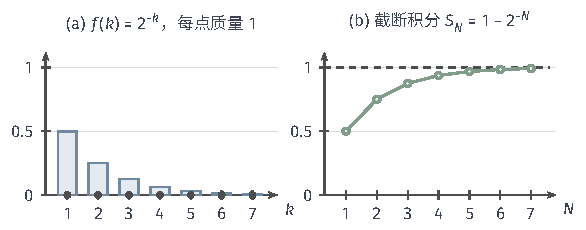
\includegraphics[width=99.24mm]{figures/02-abstract-mathematics/01-metric-and-measure/tikz/c3-counting-measure-series/figure.pdf}
 \caption{计数测度下的积分即级数。(a)$\mathbb N$上每一点（黑点）的质量为$1$，柱高为$f(k)=2^{-k}$，图中画出$k=1,\dots,7$。(b)截断$f_N=f\mathbf 1_{\{1,\dots,N\}}$的积分$S_N=1-2^{-N}$随$N$递增并趋于$1$，与单调收敛定理给出的$\int f=1$一致。}
 \label{fig:integral-counting-measure-series}
\end{figure}

\paragraph{条件收敛级数不对应积分}
定理把有限积分对应到\emph{绝对}可和，而不是对应到某种次序下收敛的级数。以$f(k)=(-1)^{k+1}/k$为例，级数$\sum_k(-1)^{k+1}/k$按原次序收敛（第~\ref{sec:integral-limits-dominated}小节将用控制收敛定理求出它的和为$\log2$），但$\sum_k|f(k)|$是发散的调和级数，所以$f$对计数测度不可积。进一步，$\int f^+=\sum_j\frac1{2j-1}$与$\int f^-=\sum_j\frac1{2j}$都是$+\infty$，$f$的积分甚至不存在。

这不是定义上的缺陷，而是测度积分不依赖次序这一要求的必然结果。计数测度上的积分是对集合$\mathbb N$赋值，集合没有“先后”；而由卷1中级数重排的讨论，条件收敛级数经过重排可以收敛到任意预先指定的实数。若把某一种次序下的和当作积分，就要在同一个测度下为同一个函数选定一种排列，这与测度的可数可加性对次序无关相矛盾。

\subsection{与黎曼积分的关系}
\label{sec:integral-riemann}

\paragraph{区间与阶梯函数}
对区间$I\subseteq[a,b]$（开、闭或半开），$\int\mathbf 1_I\,\mathrm d\lambda=\lambda(I)$等于区间长度，这与黎曼积分的值相同。端点只是零测集，开闭不影响Lebesgue积分；黎曼积分同样不受有限个点上取值的影响。由两种积分的线性，阶梯函数$\varphi=\sum_ic_i\mathbf 1_{I_i}$（$I_i$为区间）的两种积分都等于$\sum_ic_i\lambda(I_i)$。黎曼积分的上下和正是阶梯函数的积分，下面的定理就从这里把两种理论连起来。

\paragraph{Lebesgue判据}
判别有界函数是否黎曼可积，需要量化函数在一点附近的跳动幅度。设$f:[a,b]\to\mathbb R$有界，记$I_\delta(x)=(x-\delta,x+\delta)\cap[a,b]$，定义$f$在$x$处的\term{振幅}（oscillation）
\[
 \omega_f(x)=\inf_{\delta>0}\Bigl(\sup_{I_\delta(x)}f-\inf_{I_\delta(x)}f\Bigr).
\]
括号内的量随$\delta$减小而不增。$f$在$x$连续当且仅当$\omega_f(x)=0$：若连续，给定$\varepsilon$，取$\delta$使$I_\delta(x)$上$|f(y)-f(x)|<\varepsilon/2$，则括号内的量不超过$\varepsilon$；反之若$\omega_f(x)=0$，对给定$\varepsilon$取$\delta$使括号内的量小于$\varepsilon$，则$I_\delta(x)$上$|f(y)-f(x)|<\varepsilon$。于是不连续点集为$D_f=\bigcup_{m\ge1}\{\omega_f\ge1/m\}$。

\begin{theorem}[黎曼可积的Lebesgue判据]
\label{thm:integral-riemann-lebesgue}
设$f:[a,b]\to\mathbb R$有界。$f$黎曼可积，当且仅当其不连续点集$D_f$是Lebesgue零测集。此时$f$对Lebesgue可测集构成的$\sigma$代数可测，Lebesgue可积，且$\int_{[a,b]}f\,\mathrm d\lambda=\int_a^bf(x)\,\mathrm dx$。
\end{theorem}

这一判据称为\term{Lebesgue判据}（Lebesgue criterion）。证明分三步：先说明黎曼可积函数的两种积分相等，并在同一过程中得到$D_f$零测；再由$D_f$零测构造上下和之差很小的分割。设$|f|\le M$。

\begin{proof}
\emph{第一步：黎曼可积函数的Lebesgue积分。}设$f$黎曼可积。由Darboux判据，对每个$k$有分割$Q_k$使上下和之差小于$1/k$；令$P_k$为$Q_1,\dots,Q_k$的公共加细，加细不增大上下和之差，于是$P_1\subseteq P_2\subseteq\cdots$且$U(f,P_k)-L(f,P_k)\to0$。对分割$P_k$的每个小段$[x_{i-1},x_i]$，记$m_i,M_i$为$f$在其上的下、上确界，令
\[
 \varphi_k=\sum_im_i\mathbf 1_{J_i},\qquad\psi_k=\sum_iM_i\mathbf 1_{J_i},
\]
其中$J_i=[x_{i-1},x_i)$，最后一段取闭区间。于是$\varphi_k\le f\le\psi_k$处处成立，$\int\varphi_k\,\mathrm d\lambda=L(f,P_k)$，$\int\psi_k\,\mathrm d\lambda=U(f,P_k)$。分割加细时子段上的下确界不减、上确界不增，所以$\varphi_k$递增、$\psi_k$递减，分别有逐点极限$\varphi\le f\le\psi$，它们是Borel可测函数。

由$0\le\psi-\varphi\le\psi_k-\varphi_k$，$\int(\psi-\varphi)\le U(f,P_k)-L(f,P_k)\to0$，故$\int(\psi-\varphi)=0$，由引理~\ref{lem:integral-nonnegative-basic}第4条，$\psi=\varphi$在零测集$N$外成立，从而$f=\varphi$在$N$外成立。对任意$t$，$\{f>t\}$与Borel集$\{\varphi>t\}$只在$N$内可能不同；$(\mathbb R,\mathcal L,\lambda)$完备，所以$f$对$\mathcal L$可测。又$|f|\le M$且区间测度有限，$f$可积。$\varphi_k+M\ge0$递增到$\varphi+M$，单调收敛定理给出$\int(\varphi_k+M)\to\int(\varphi+M)$，两边减去有限数$M(b-a)$得
\[
 \int_{[a,b]}f\,\mathrm d\lambda=\int_{[a,b]}\varphi\,\mathrm d\lambda=\lim_kL(f,P_k)=\int_a^bf(x)\,\mathrm dx.
\]

\emph{第二步：黎曼可积蕴含$D_f$零测。}全部分割$P_k$的分点只有可数个，组成零测集$Z$。若$x\notin Z$，对每个$k$，$x$位于$P_k$某个小段的内部，存在$\delta$使$I_\delta(x)$包含于该小段，于是$\omega_f(x)\le M_i-m_i=\psi_k(x)-\varphi_k(x)$。令$k\to\infty$得$\omega_f(x)\le\psi(x)-\varphi(x)$。在零测集$Z\cup N$之外右端为零，所以$D_f=\{\omega_f>0\}\subseteq Z\cup N$，是零测集。

\emph{第三步：$D_f$零测蕴含黎曼可积。}给定$\varepsilon>0$，令$K=\{\omega_f\ge\varepsilon\}$。$K$是闭集：若$\omega_f(x)<\varepsilon$，取$\delta$使$I_\delta(x)$上上下确界之差小于$\varepsilon$，则对$|y-x|<\delta/2$，$I_{\delta/2}(y)\subseteq I_\delta(x)$，故$\omega_f(y)<\varepsilon$，即$\{\omega_f<\varepsilon\}$在$[a,b]$中相对开。$K\subseteq D_f$是零测的有界闭集，由外测度的定义可用可数个开区间覆盖$K$且总长小于$\varepsilon$；$K$紧致，取其中有限个，记其并为$G$，它由有限个两两不交的开区间组成，总长小于$\varepsilon$。

$[a,b]\setminus G$是有限个闭区间$H_1,\dots,H_r$之并，其上处处$\omega_f<\varepsilon$。对每点$x\in H_l$取$\delta_x$使$I_{\delta_x}(x)$上的上下确界之差小于$\varepsilon$；区间$(x-\delta_x/2,x+\delta_x/2)$覆盖紧集$H_l$，取有限子覆盖，令$\delta$为相应$\delta_x/2$的最小值。若$H_l$中的小段$J$长度小于$\delta$，取$y\in J$，$y$落在某个$(x-\delta_x/2,x+\delta_x/2)$中，则$J\subseteq I_{\delta_x}(x)$，$f$在$J$上的上下确界之差小于$\varepsilon$。把每个$H_l$分成长度小于$\delta$的小段，再加上$G$各分支与$[a,b]$之交的端点，得到分割$P$。$P$的小段分两类：落在某个$H_l$中的，上下确界之差小于$\varepsilon$，总长不超过$b-a$；落在$G$某个分支闭包中的，上下确界之差不超过$2M$，总长小于$\varepsilon$。所以
\[
 U(f,P)-L(f,P)<\varepsilon(b-a)+2M\varepsilon,
\]
由$\varepsilon$的任意性与Darboux判据，$f$黎曼可积。
\end{proof}

第一步说明两种理论在共同范围内一致：黎曼可积函数的上下阶梯函数从两侧夹住它，Lebesgue积分只是记录了夹逼的公共极限。第二、三步说明黎曼可积的障碍恰好是不连续点占据正的长度。这里用到完备性：$f$未必Borel可测，但与Borel函数仅在零测集上不同。

\paragraph{Dirichlet函数}
在$[0,1]$上，有理点示性函数$\mathbf 1_{\mathbb Q}$称为\term{Dirichlet函数}（Dirichlet function）。$\mathbb Q\cap[0,1]$可数，Lebesgue测度为零，所以$\int_{[0,1]}\mathbf 1_{\mathbb Q}\,\mathrm d\lambda=0$。另一方面，有理点与无理点都在$[0,1]$中稠密，每个小区间上$\mathbf 1_{\mathbb Q}$的上确界为$1$、下确界为$0$，振幅处处为$1$，$D_f=[0,1]$的测度为$1$，由Lebesgue判据它不黎曼可积；这与卷1中“任意分割的下和为$0$、上和为$1$”的计算一致。图~\ref{fig:integral-dirichlet-function}(a)用两条点线示意这种处处跳动。

\begin{figure}[!htbp]
 \centering
 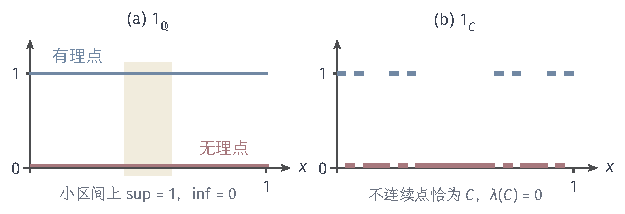
\includegraphics[width=105.876mm]{figures/02-abstract-mathematics/01-metric-and-measure/tikz/c3-dirichlet-function/figure.pdf}
 \caption{两种不连续点集。(a)Dirichlet函数$\mathbf 1_{\mathbb Q}$在有理点取$1$（蓝）、无理点取$0$（红），两类点都稠密，任一小区间（黄色带）上上确界为$1$、下确界为$0$，不连续点集为整个$[0,1]$。(b)Cantor集示性函数$\mathbf 1_C$，用第三步的$8$个保留区间示意$C$；它在$C$外的开区间上恒为零而连续，不连续点恰为$C$，$\lambda(C)=0$，所以黎曼可积且积分为$0$。}
 \label{fig:integral-dirichlet-function}
\end{figure}

这个例子同时区分了稠密与零测：$\mathbb Q\cap[0,1]$稠密却零测，函数在它上面的取值对Lebesgue积分毫无影响，对黎曼积分却是致命的，因为黎曼上下和在每个小区间上都会“看到”有理点。图(b)给出另一侧的对照。Cantor集$C$（例~\ref{ex:measure-cantor-set}）是零测的闭集，$\mathbf 1_C$在每个$x\notin C$的邻域内恒为零，因而连续；在$x\in C$处，$C$不含任何区间，$x$附近有取值为零的点，因而不连续。于是$D_f=C$不可数却零测，$\mathbf 1_C$黎曼可积，两种积分都是$0$。决定黎曼可积性的是不连续点集的测度，而不是它的基数或稠密性；Lebesgue积分则根本不要求函数在小区间上近似为常数，只要求各层可测。

\subsection{与反常积分的关系}
\label{sec:integral-improper}

\paragraph{截断与单调收敛}
反常积分处理两种情形：区间无界，或函数在端点附近无界。两者的做法相同：先在有限闭区间上作黎曼积分，再让区间扩张取极限。对非负函数，截断区间上的积分随区间扩张递增，这正是单调收敛定理的情形。

\begin{theorem}[反常积分与Lebesgue积分]
\label{thm:integral-improper}
设$-\infty<a<\beta\le+\infty$，$I=[a,\beta)$，$f:I\to\mathbb R$在每个$[a,b]$（$a<b<\beta$）上黎曼可积。
\begin{enumerate}
 \item 若$f\ge0$，则$\int_If\,\mathrm d\lambda=\lim_{b\uparrow\beta}\int_a^bf(x)\,\mathrm dx$，两边在$[0,+\infty]$中相等。
 \item $f$在$I$上Lebesgue可积，当且仅当反常积分$\int_a^\beta|f(x)|\,\mathrm dx$收敛，即$\int_a^\beta f$绝对收敛；此时$\int_If\,\mathrm d\lambda=\int_a^\beta f(x)\,\mathrm dx$。
\end{enumerate}
左端点为奇点的区间$(\alpha,b]$与两端都需截断的区间可类似处理。
\end{theorem}

\begin{proof}
取$b_n\uparrow\beta$。由定理~\ref{thm:integral-riemann-lebesgue}，每个$f\mathbf 1_{[a,b_n]}$对$\mathcal L$可测，它们逐点收敛到$f\mathbf 1_I$，所以$f$在$I$上可测。

第1条：$f\ge0$时$f\mathbf 1_{[a,b_n]}\uparrow f\mathbf 1_I$，单调收敛定理与定理~\ref{thm:integral-riemann-lebesgue}给出$\int_If\,\mathrm d\lambda=\lim_n\int_a^{b_n}f\,\mathrm dx$。由于$b\mapsto\int_a^bf$递增，沿任意$b_n\uparrow\beta$的极限都等于$b\uparrow\beta$时的极限。

第2条：$|f|$在每个$[a,b]$上黎曼可积（其振幅不超过$f$的振幅），由第1条$\int_I|f|\,\mathrm d\lambda=\lim_{b\uparrow\beta}\int_a^b|f|$，可积性的等价随之成立。可积时$f^\pm=\frac12(|f|\pm f)$也在每个$[a,b]$上黎曼可积，由第1条$\int_If^\pm\,\mathrm d\lambda=\lim_b\int_a^bf^\pm$，两个极限都有限，相减得$\int_If\,\mathrm d\lambda=\lim_b\int_a^bf$。
\end{proof}

于是对非负函数，反常积分收敛与Lebesgue可积是同一回事，值也相同；例如$\int_{(0,1]}x^{-1/2}\,\mathrm dx=\lim_{\varepsilon\downarrow0}(2-2\sqrt\varepsilon)=2$，$\int_{[1,+\infty)}x^{-2}\,\mathrm dx=\lim_b(1-1/b)=1$，$\int_{[0,+\infty)}\mathrm e^{-x}\,\mathrm dx=\lim_b(1-\mathrm e^{-b})=1$。对可正可负的函数，两种理论在绝对收敛时一致；复值函数对实部和虚部分别使用第2条。

\paragraph{条件收敛的反常积分}
反常积分只要求截断积分有极限，允许正负部分相互抵消；Lebesgue积分则要求正负两部分各自有限。$f(x)=\sin x/x$在$[1,+\infty)$上体现了这一区别。按卷1中分部积分的论证，$\int_1^b\sin x/x\,\mathrm dx$在$b\to+\infty$时收敛，所以反常积分存在。但在第$k$瓣$[k\pi,(k+1)\pi]$（$k\ge1$）上$|\sin x|/x\ge|\sin x|/((k+1)\pi)$，而$\int_{k\pi}^{(k+1)\pi}|\sin x|\,\mathrm dx=2$，所以
\[
 \int_{[1,+\infty)}\frac{|\sin x|}x\,\mathrm dx\ge\sum_{k=1}^\infty\frac2{(k+1)\pi}=+\infty.
\]
由定理~\ref{thm:integral-improper}，$f$不Lebesgue可积；进一步，$\int f^+$与$\int f^-$都是$+\infty$：由定理~\ref{thm:integral-improper}第1条，它们分别是$\int_1^bf^\pm$在$b\to+\infty$时的极限，而$\int_1^bf^+-\int_1^bf^-=\int_1^bf$有有限极限，若其中一个有限，另一个也有限，与$\int|f|=+\infty$矛盾。因此$f$在$[1,+\infty)$上的Lebesgue积分不存在。

图~\ref{fig:integral-sinc-improper}显示了原因：正瓣与负瓣交替出现，面积按$1/k$缓慢减小。反常积分按从左到右的次序累加，正负瓣两两抵消，部分和收敛；把正瓣和负瓣分别累加，各自都是发散的调和型级数。这与上一小节条件收敛级数的情形一致：反常积分的值依赖“沿$x$增大的方向截断”这一特定次序，测度积分不使用任何次序。

\begin{figure}[!htbp]
 \centering
 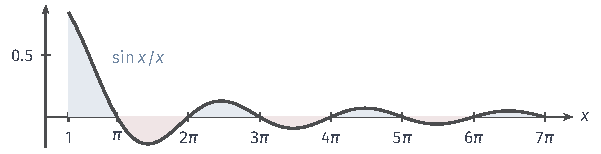
\includegraphics[width=101.699mm]{figures/02-abstract-mathematics/01-metric-and-measure/tikz/c3-sinc-improper/figure.pdf}
 \caption{$f(x)=\sin x/x$在$[1,7\pi]$上的图像，正瓣为蓝、负瓣为红。第$k$瓣$[k\pi,(k+1)\pi]$上$|f|$的面积不小于$2/((k+1)\pi)$，各瓣面积之和按调和级数发散，所以$f$在$[1,+\infty)$上不Lebesgue可积；按$x$增大的次序累加时正负瓣相互抵消，反常积分收敛。}
 \label{fig:integral-sinc-improper}
\end{figure}

\paragraph{Cauchy主值}
在内部奇点两侧，还有一种更依赖次序的规定。$f(x)=1/x$在$[-1,1]\setminus\{0\}$上，两侧同步截断得
\[
 \lim_{\varepsilon\downarrow0}\Bigl(\int_{-1}^{-\varepsilon}\frac{\mathrm dx}x+\int_\varepsilon^1\frac{\mathrm dx}x\Bigr)=\lim_{\varepsilon\downarrow0}(\log\varepsilon-\log\varepsilon)=0,
\]
这称为\term{Cauchy主值}（Cauchy principal value）。若右侧改为从$2\varepsilon$截断，同样的计算得到$\log\varepsilon-\log(2\varepsilon)=-\log2$，可见结果取决于两侧逼近的速度之比。通常的反常积分要求两侧分别取极限，而$\int_\varepsilon^1\mathrm dx/x=-\log\varepsilon\to+\infty$，所以它发散；Lebesgue积分中$\int f^+=\int f^-=+\infty$，积分不存在。主值是在特定问题中额外指定的抵消规则，不能当作反常积分或Lebesgue积分的值。

\section{积分与极限}
\label{sec:integral-limits}

函数列逐点收敛时，积分未必随之收敛：前面的例子已经显示，逐点趋于零的函数可以保持积分为一。本节固定测度$\mu$，研究函数列或函数项级数在什么条件下允许交换积分与极限。各小节按可以核查的条件组织：非负且递增；只有非负；所有项受同一个可积函数控制；各项绝对积分之和有限；以及有限测度上的一致收敛。每个条件下给出相应的定理和使用方式，并用反例说明去掉条件后哪里出错。测度本身随参数变化时积分怎样收敛，是另一类问题，留待后文讨论测度序列的收敛时处理。

\subsection{非负递增条件下的极限交换}
\label{sec:integral-limits-monotone}

\paragraph{递增列}
第~\ref{sec:integral-mct}小节的单调收敛定理（定理~\ref{thm:integral-monotone-convergence}）已经回答了最简单的情形：若$0\le f_1\le f_2\le\cdots$可测且逐点趋于$f$，则$\int f_n\to\int f$，共同结果可以是$+\infty$。核查条件时只需确认两点：各项非负，且逐点递增（允许在零测集外成立）。不需要任何可积性，这是它与后面几种条件的主要区别。下面把它用于两种常见操作，它们都归结为同一个非负递增条件。

\begin{theorem}[非负级数的逐项积分与递增区域]
\label{thm:integral-series-nonnegative}
\begin{enumerate}
 \item 设$g_1,g_2,\dots:X\to[0,+\infty]$可测，则$\int_X\sum_{k=1}^\infty g_k\,\mathrm d\mu=\sum_{k=1}^\infty\int_Xg_k\,\mathrm d\mu$。
 \item 设$f\ge0$可测，$E_1\subseteq E_2\subseteq\cdots$可测，$E=\bigcup_nE_n$，则$\int_{E_n}f\,\mathrm d\mu\to\int_Ef\,\mathrm d\mu$。
 \item 设$f\ge0$可测，则$\nu(E)=\int_Ef\,\mathrm d\mu$定义$(X,\mathcal A)$上的测度。
\end{enumerate}
\end{theorem}

\begin{proof}
第1条：部分和$S_N=\sum_{k\le N}g_k$非负、递增，逐点趋于$\sum_kg_k$；由非负积分的加法$\int S_N=\sum_{k\le N}\int g_k$，再用单调收敛定理。第2条：$f\mathbf 1_{E_n}\uparrow f\mathbf 1_E$，用单调收敛定理。第3条：$\nu(\varnothing)=0$；若$E_k$两两不交，则$f\mathbf 1_{\bigcup_kE_k}=\sum_kf\mathbf 1_{E_k}$，由第1条得可数可加性。
\end{proof}

第3条中的测度$\nu$把每个区域上的累计值记录下来，它在$\mu$-零测集上取零（引理~\ref{lem:integral-nonnegative-basic}第3条）。反过来，哪些测度能写成这种形式，是第~\ref{chap:densities-change-of-measure}章的主题。

\paragraph{两个计算}
在$(0,1)$上，$-\log(1-x)/x=\sum_{k\ge1}x^{k-1}/k$，各项非负。由$\int_0^1x^{k-1}/k\,\mathrm dx=1/k^2$与第1条，
\[
 \int_{(0,1)}\frac{-\log(1-x)}x\,\mathrm dx=\sum_{k=1}^\infty\frac1{k^2}\le1+\sum_{k\ge2}\frac1{k(k-1)}=2,
\]
所以这个在$x\to1$处无界的函数可积（级数的值为$\pi^2/6$，这一经典结果此处用不到）。对递增区域，取$E_n=[1,n]$，$\int_{E_n}x^{-2}\,\mathrm dx=1-1/n\to1$，这就是上一节反常积分结论的来源。两种操作中，若结果为$+\infty$，等式同样成立：$\sum_{k\ge0}x^k=1/(1-x)$在$[0,1)$上逐项积分，左边$\int_0^1\mathrm dx/(1-x)=+\infty$，右边$\sum_k1/(k+1)=+\infty$。

\subsection{非负条件下的积分下界}
\label{sec:integral-limits-fatou}

\paragraph{Fatou引理}
当非负函数列不再递增时，可以先构造一列递增的下界。尾部下确界$g_n=\inf_{k\ge n}f_k$随$n$递增，并趋于$\liminf_nf_n$；对它用单调收敛定理，就得到下面的不等式。

\begin{lemma}[Fatou引理]
\label{lem:integral-fatou}
设$f_1,f_2,\dots:X\to[0,+\infty]$可测，则
\[
 \int_X\liminf_{n\to\infty}f_n\,\mathrm d\mu\le\liminf_{n\to\infty}\int_Xf_n\,\mathrm d\mu.
\]
这一结论称为\term{Fatou引理}（Fatou's lemma）。
\end{lemma}

\begin{proof}
令$g_n=\inf_{k\ge n}f_k$，由定理~\ref{thm:measure-limits}可测，$0\le g_1\le g_2\le\cdots$，且$\sup_ng_n=\liminf_nf_n$。对每个$k\ge n$有$g_n\le f_k$，故$\int g_n\le\int f_k$，从而$\int g_n\le\inf_{k\ge n}\int f_k$。由单调收敛定理，
\[
 \int\liminf_nf_n=\lim_n\int g_n\le\lim_n\inf_{k\ge n}\int f_k=\liminf_n\int f_n.
\]
\end{proof}

引理不要求$f_n$逐点收敛，也不要求可积；它只给出“先取极限再积分”的一个下界。若$f_n$逐点收敛到$f$，结论读作$\int f\le\liminf\int f_n$：极限函数的积分不会超过积分的下极限，但可能更小。

\paragraph{丢失的积分质量}
在实轴上取$f_n=\mathbf 1_{[n,n+1]}$。固定$x$，当$n>x$时$f_n(x)=0$，所以$f_n$逐点趋于$0$，左边为$0$；而每个$\int f_n\,\mathrm d\lambda=1$，右边为$1$，不等式严格成立。图~\ref{fig:integral-escaping-mass}(a)显示，单位质量整体向远处平移，每个固定的点最终都看不到它，点态极限因此丢失了全部积分质量。

\begin{figure}[!htbp]
 \centering
 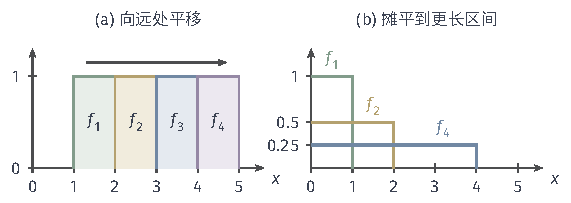
\includegraphics[width=96.629mm]{figures/02-abstract-mathematics/01-metric-and-measure/tikz/c3-escaping-mass/figure.pdf}
 \caption{积分质量从点态极限中丢失的两种方式。(a)$f_n=\mathbf 1_{[n,n+1]}$（$n=1,2,3,4$）向远处平移，逐点趋于零而每项积分为$1$。(b)$f_n=n^{-1}\mathbf 1_{[0,n]}$（$n=1,2,4$）摊平到越来越长的区间，$\sup|f_n|=1/n$一致趋于零而每项积分仍为$1$。}
 \label{fig:integral-escaping-mass}
\end{figure}

非负性也不能去掉：把上例换成$-f_n$，点态极限的积分为$0$，而$\liminf\int(-f_n)=-1$，不等式反向。只有非负性时，通常只能得到下界；要把不等式变为等式，需要阻止质量逃逸。下一小节的统一控制条件正是为此而设。

\subsection{可积控制条件下的极限交换}
\label{sec:integral-limits-dominated}

\paragraph{控制收敛定理}
若所有$|f_n|$都被同一个可积函数$g$压住，质量就无处可逃：$g$本身的积分有限，任何试图跑到远处或集中到窄峰的质量都受$g$在那里的取值约束。证明的办法是对非负函数$2g-|f_n-f|$应用Fatou引理。

\begin{theorem}[控制收敛定理]
\label{thm:integral-dominated-convergence}
设$f_n$、$f$是实值或复值可测函数，$g\ge0$可积，满足：$f_n\to f$ $\mu$-几乎处处；对每个$n$，$|f_n|\le g$ $\mu$-几乎处处。则$f$可积，
\[
 \lim_{n\to\infty}\int_X|f_n-f|\,\mathrm d\mu=0,\qquad\lim_{n\to\infty}\int_Xf_n\,\mathrm d\mu=\int_Xf\,\mathrm d\mu.
\]
这一结论称为\term{控制收敛定理}（dominated convergence theorem），$g$称为控制函数。
\end{theorem}

\begin{proof}
\emph{合并例外集。}按定义，收敛与每个不等式$|f_n|\le g$各在某个零测集外成立；再加上$\{g=+\infty\}$，它由引理~\ref{lem:integral-nonnegative-basic}第5条是零测集。这些例外集只有可数个，其并$N$仍是零测集。把$f_n,f,g$都乘以$\mathbf 1_{X\setminus N}$，函数仍可测，各积分不变（引理~\ref{lem:integral-nonnegative-basic}第3条），而现在收敛与控制在每一点成立，$g$处处有限。

\emph{极限函数可积。}由$|f_n|\le g$及逐点收敛，$|f|\le g$，故$f$可积。

\emph{应用Fatou引理。}$|f_n-f|\le|f_n|+|f|\le2g$，所以$h_n=2g-|f_n-f|$是非负可测函数，且逐点趋于$2g$。由Fatou引理，
\[
 \begin{aligned}
  \int2g&\le\liminf_n\int h_n=\liminf_n\Bigl(\int2g-\int|f_n-f|\Bigr)\\
  &=\int2g-\limsup_n\int|f_n-f|,
 \end{aligned}
\]
其中第一个等号用了可积函数的线性，所有量都有限。消去有限数$\int2g$，得$\limsup_n\int|f_n-f|\le0$，即$\int|f_n-f|\to0$。最后由绝对值估计，$\bigl|\int f_n-\int f\bigr|\le\int|f_n-f|\to0$。
\end{proof}

证明中“消去$\int2g$”一步要求它有限，这正是控制函数必须可积的原因；而合并例外集只用到可数个零测集之并仍是零测集。积分绝对误差$\int|f_n-f|\,\mathrm d\mu$在这里只是一个数，它趋于零比积分本身收敛更强；把它作为函数空间的距离来研究，属于后面讨论$L^1$空间时的内容。

\paragraph{一个可控与一个不可控的例子}
在$[0,+\infty)$上令
\[
 f_n(x)=(1-x/n)^n\mathbf 1_{[0,n]}(x).
\]
对固定的$x$，当$n>x$时$f_n(x)=(1-x/n)^n\to\mathrm e^{-x}$。又由$\log(1-t)\le-t$（$0\le t<1$），$0\le f_n(x)\le\mathrm e^{-x}$，而$\mathrm e^{-x}$在$[0,+\infty)$上可积，积分为$1$（第~\ref{sec:integral-improper}小节）。控制收敛定理给出$\int_0^n(1-x/n)^n\,\mathrm dx\to1$；直接计算，代换$u=1-x/n$得$\int_0^n(1-x/n)^n\,\mathrm dx=n\int_0^1u^n\,\mathrm du=n/(n+1)$，确实趋于$1$。

反过来，在$[0,1]$上取$f_n=n\mathbf 1_{(0,1/n)}$，各项可积且积分恒为$1$，并在每一点趋于$0$，但积分的极限$1$不等于$0$。定理失效是因为找不到可积的控制函数：任何控制函数都不小于上包络$h=\sup_nf_n$，而在$[\frac1{n+1},\frac1n)$上$h=n$，故$h(x)\ge1/x-1$，$\int_0^1(1/x-1)\,\mathrm dx=+\infty$。图~\ref{fig:integral-dominating-envelope}对比了两种情形：(a)中$f_n=x^n$都在可积的常数$1$之下，$\int x^n=1/(n+1)\to0$与点态极限（几乎处处为$0$）的积分一致；(b)中窄而高的矩形把质量集中到原点附近，它们的上包络已不可积。

\begin{figure}[!htbp]
 \centering
 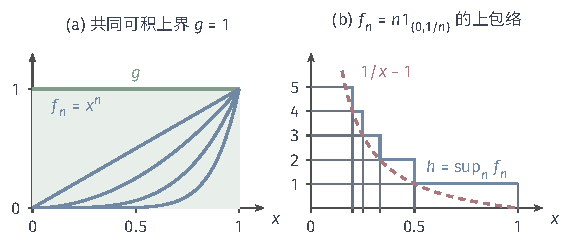
\includegraphics[width=96.633mm]{figures/02-abstract-mathematics/01-metric-and-measure/tikz/c3-dominating-envelope/figure.pdf}
 \caption{控制函数与上包络。(a)$[0,1]$上$f_n=x^n$（$n=1,2,4,8$）都位于可积函数$g=1$之下，积分$1/(n+1)\to0$。(b)$f_n=n\mathbf 1_{(0,1/n)}$（灰色，$n=1,\dots,5$）积分恒为$1$；上包络$h=\sup_nf_n$（蓝色阶梯）在$[\frac1{n+1},\frac1n)$上等于$n$，不小于$1/x-1$（红色虚线），后者在$(0,1)$上积分为$+\infty$，所以不存在可积的控制函数。}
 \label{fig:integral-dominating-envelope}
\end{figure}

\paragraph{函数项级数}
对级数$\sum_kf_k$，把部分和记为$S_N=\sum_{k\le N}f_k$。若$S_N$几乎处处收敛，并且所有$|S_N|$受同一个可积函数控制，就对部分和应用定理，得到$\int\sum_kf_k=\sum_k\int f_k$。需要控制的是部分和，不是单项：在$[0,1]$上取$f_k=\frac1k\mathbf 1_{[0,1]}$，每一项都不超过可积函数$1$，部分和却是调和级数的部分和，逐点发散。

交错几何级数是一个部分和受控而单项绝对积分不可和的例子。在$[0,1)$上，$S_N(x)=\sum_{k=0}^N(-x)^k=\frac{1-(-x)^{N+1}}{1+x}$，满足$|S_N|\le2$，并逐点收敛到$1/(1+x)$。常数$2$在$[0,1)$上可积，所以
\[
 \sum_{k=0}^\infty\frac{(-1)^k}{k+1}=\sum_{k=0}^\infty\int_0^1(-x)^k\,\mathrm dx=\int_0^1\frac{\mathrm dx}{1+x}=\log2.
\]
这同时求出了第~\ref{sec:integral-discrete-sums}小节交错调和级数按原次序的和。注意每一项的绝对积分为$1/(k+1)$，对$k$求和得$+\infty$，下一小节的条件在这里并不成立；控制部分和是比它更细的论证。

\subsection{绝对积分可和条件下的逐项积分}
\label{sec:integral-limits-absolute-series}

\paragraph{逐项检查的条件}
构造部分和的控制函数往往要先知道级数的和。下面的条件只需逐项计算积分，并且自动提供控制函数与截断误差。

\begin{theorem}[绝对积分可和时的逐项积分]
\label{thm:integral-absolute-series}
设$f_1,f_2,\dots$是实值或复值可测函数，且$\sum_{n=1}^\infty\int_X|f_n|\,\mathrm d\mu<+\infty$。则$\sum_n|f_n(x)|<+\infty$对$\mu$-几乎所有$x$成立；在这些点上令$f(x)=\sum_nf_n(x)$，其余点令$f(x)=0$，则$f$可积，
\[
 \int_Xf\,\mathrm d\mu=\sum_{n=1}^\infty\int_Xf_n\,\mathrm d\mu,\qquad\int_X\Bigl|f-\sum_{n\le N}f_n\Bigr|\,\mathrm d\mu\le\sum_{n>N}\int_X|f_n|\,\mathrm d\mu.
\]
这种交换称为\term{逐项积分}（termwise integration）。
\end{theorem}

\begin{proof}
令$G=\sum_n|f_n|$。由定理~\ref{thm:integral-series-nonnegative}第1条，$\int G=\sum_n\int|f_n|<+\infty$，再由引理~\ref{lem:integral-nonnegative-basic}第5条，$G$几乎处处有限。在可测集$\{G<+\infty\}$上级数绝对收敛，因而收敛；$f$是部分和的逐点极限乘以该集合的示性函数，可测。部分和$S_N$满足$|S_N|\le G$，$G$可积，由控制收敛定理得$\int S_N\to\int f$，即$\sum_{n\le N}\int f_n\to\int f$。余项估计：在$\{G<+\infty\}$上$|f-S_N|\le\sum_{n>N}|f_n|$，对右端再用定理~\ref{thm:integral-series-nonnegative}第1条。
\end{proof}

条件$\sum_n\int|f_n|<+\infty$同时完成了三件事：说明级数几乎处处绝对收敛，给出控制函数$G$，并给出截断误差的上界。它比上一小节对部分和的控制要求更强，但更容易验证。

\paragraph{一个带误差的计算}
在$(0,1)$上，$\frac{\log(1+x)}x=\sum_{n\ge1}(-1)^{n+1}\frac{x^{n-1}}n$。各项满足$\int_0^1\bigl|\frac{x^{n-1}}n\bigr|\,\mathrm dx=\frac1{n^2}$，其和有限，定理适用：
\[
 \int_0^1\frac{\log(1+x)}x\,\mathrm dx=\sum_{n=1}^\infty\frac{(-1)^{n+1}}{n^2}.
\]
保留前$N$项时，误差不超过$\sum_{n>N}\frac1{n^2}\le\sum_{n>N}\frac1{n(n-1)}=\frac1N$。例如取前$10$项，积分值与$\sum_{n\le10}(-1)^{n+1}/n^2$之差不超过$0.1$；实际误差还要小得多，这里的上界只用到逐项的绝对积分。

\subsection{有限测度与一致收敛条件下的极限交换}
\label{sec:integral-limits-uniform}

\paragraph{统一误差乘以总测度}
卷1在闭区间上证明过：一致收敛的黎曼可积函数列可以逐项积分，关键是“统一误差乘以区间长度”。在一般测度空间上，区间长度换成总测度，论证同样成立。

\begin{theorem}[有限测度上的一致收敛]
\label{thm:integral-uniform-finite}
设$\mu(X)<+\infty$，$f_n$是实值或复值可积函数，且在$X$上一致收敛到$f$，即$\sup_X|f_n-f|\to0$。则$f$可积，并且
\[
 \int_X|f_n-f|\,\mathrm d\mu\le\mu(X)\sup_X|f_n-f|\to0,\qquad\int_Xf_n\,\mathrm d\mu\to\int_Xf\,\mathrm d\mu.
\]
\end{theorem}

\begin{proof}
$f$是可测函数列的逐点极限，可测。取$N$使$\sup_X|f-f_N|\le1$，则$|f|\le|f_N|+1$，而$|f_N|$与常数$1$在有限测度空间上都可积，故$f$可积。对每个$n$，$|f_n-f|\le\sup_X|f_n-f|$，积分后得估计式；再由绝对值估计得积分收敛。
\end{proof}

定理要求每一项都可积，这在证明的最后一步使用：估计$\bigl|\int f_n-\int f\bigr|$时，$\int f_n$必须是有限数。例如在$[0,1]$上，$\sum_{k\le n}x^k/k!$一致收敛到$\mathrm e^x$，于是$\int_0^1\mathrm e^x\,\mathrm dx=\lim_n\sum_{k\le n}\frac1{(k+1)!}=\mathrm e-1$。

\paragraph{无限测度上的反例}
有限测度不可省略。在$[0,+\infty)$上取$f_n=n^{-1}\mathbf 1_{[0,n]}$，则$\sup|f_n|=1/n\to0$，函数列一致收敛到$0$，而每个$\int f_n\,\mathrm d\lambda=1$。图~\ref{fig:integral-escaping-mass}(b)显示，质量没有集中，而是摊平到越来越长的区间上；统一误差$1/n$乘以支撑区间的长度$n$恰好保持为$1$。与(a)的平移相比，这里连逐点误差的上确界都趋于零，失败完全来自总测度无限。

本节五类条件各有用途：单调收敛不要求可积，允许结果为无穷；Fatou引理只要求非负，给出下界；控制收敛要求一个共同的可积上界，是最常用的一般工具；绝对积分可和便于逐项检查并附带误差估计；有限测度上的一致收敛最容易验证，但适用范围最窄。图~\ref{fig:integral-escaping-mass}与图~\ref{fig:integral-dominating-envelope}中的反例分别对应质量逃逸到远处、摊平到无限测度和集中到窄峰三种失效方式。

\section{累次积分}
\label{sec:integral-iterated}

矩形的面积等于两条边长之积；求一块区域上的总量时，我们也习惯先沿每条竖线累计，再把各条竖线的结果横向相加。前几节的积分只用到一个测度空间。现在有两个测度空间$(X,\mathcal A,\mu)$与$(Y,\mathcal B,\nu)$，需要回答两个问题：乘积集合$X\times Y$上的“面积”怎样由两侧的测度确定；分别对两个坐标累计，什么时候等于整体累计，两种累计次序又何时相同。本节先建立乘积可测结构和乘积测度，再分别给出非负函数与绝对可积函数的换序定理，最后把它们用于欧氏空间中的多重积分和截面计算。

\subsection{乘积可测结构与乘积测度}
\label{sec:integral-product-measure}

\paragraph{可测矩形与乘积\texorpdfstring{$\sigma$}{sigma}代数}
两侧各取一个可测集$A\in\mathcal A$、$B\in\mathcal B$，乘积$A\times B$是最容易确定大小的集合：它的“面积”理应是$\mu(A)\nu(B)$。但圆盘、三角形这类集合都不是这种形式，乘积空间上的可测集合必须由矩形生成。

\begin{definition}[乘积$\sigma$代数]
\label{def:integral-product-sigma-algebra}
设$(X,\mathcal A)$与$(Y,\mathcal B)$是可测空间。形如$A\times B$（$A\in\mathcal A$，$B\in\mathcal B$）的集合称为\term{可测矩形}（measurable rectangle）。由全部可测矩形生成的$\sigma$代数记为$\mathcal A\otimes\mathcal B$，称为\term{乘积$\sigma$代数}（product sigma-algebra）。
\end{definition}

可测矩形全体对有限交封闭：$(A_1\times B_1)\cap(A_2\times B_2)=(A_1\cap A_2)\times(B_1\cap B_2)$。因此它是一个$\pi$系统，后面可以用第二章的$\pi$--$\lambda$定理（定理~\ref{thm:measure-pi-lambda}）比较两个在矩形上取值相同的测度。图~\ref{fig:integral-product-rectangles}(a)中$A$由两个区间组成，矩形$A\times B$因而是两块；(b)说明四分之一圆盘虽然不是矩形，却可以由互不重叠的小矩形逐层填满，成为可数个矩形之并。

\begin{figure}[!htbp]
\centering
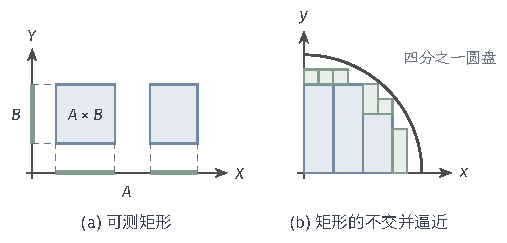
\includegraphics[width=85.93mm]{figures/02-abstract-mathematics/01-metric-and-measure/tikz/c3-product-rectangles/figure.pdf}
\caption{乘积可测结构由矩形生成。(a)取$A=[0.4,1.4]\cup[2.0,2.8]$、$B=[0.5,1.5]$，可测矩形$A\times B$由两块组成，绿色线段分别是$A$与$B$；(b)半径为$2$的四分之一圆盘不是矩形，蓝色矩形按边长$0.5$的网格、绿色矩形按边长$0.25$的网格补充，逐层加细的矩形不交并从内部逼近圆盘。}
\label{fig:integral-product-rectangles}
\end{figure}

\paragraph{截面}
累次积分先固定一个坐标。对$E\subseteq X\times Y$和$x\in X$，称
\[
 E_x=\{y\in Y:(x,y)\in E\}
\]
为$E$在$x$处的\term{截面}（section）；类似地，$E^y=\{x\in X:(x,y)\in E\}$是$E$在$y$处的截面。对函数$f:X\times Y\to\overline{\mathbb R}$，固定$x$得到截面函数$f_x(y)=f(x,y)$，固定$y$得到$f^y(x)=f(x,y)$。图~\ref{fig:integral-sections}中的区域在$x_0$处的截面是一段区间，在$y_0$处的截面却是两段区间：截面的形状取决于固定哪个坐标。

\begin{figure}[!htbp]
\centering
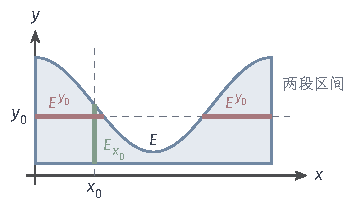
\includegraphics[width=60.187mm]{figures/02-abstract-mathematics/01-metric-and-measure/tikz/c3-sections/figure.pdf}
\caption{同一集合沿两个方向的截面。区域$E=\{(x,y):0\le x\le4,\ 0.2\le y\le1.2+0.8\cos(\pi x/2)\}$；绿色竖线是$x_0=1$处的截面$E_{x_0}=[0.2,1.2]$，红色横线是$y_0=1$处的截面$E^{y_0}$，由$\cos(\pi x/2)\ge-0.25$解得它约为$[0,1.161]\cup[2.839,4]$。}
\label{fig:integral-sections}
\end{figure}

截面运算与集合运算可交换：$(E^{c})_x=(E_x)^{c}$，$(\bigcup_nE_n)_x=\bigcup_n(E_n)_x$。矩形的截面最简单，$(A\times B)_x$在$x\in A$时是$B$，否则是空集。由这两点即可证明乘积可测集的每个截面都可测。

\begin{lemma}[截面可测]
\label{lem:integral-section-measurable}
若$E\in\mathcal A\otimes\mathcal B$，则对每个$x\in X$有$E_x\in\mathcal B$，对每个$y\in Y$有$E^y\in\mathcal A$。若$f$是$\mathcal A\otimes\mathcal B$可测函数，则每个$f_x$是$\mathcal B$可测的，每个$f^y$是$\mathcal A$可测的。
\end{lemma}

\begin{proof}
固定$x$，令$\mathcal C=\{E\in\mathcal A\otimes\mathcal B:E_x\in\mathcal B\}$。上面的两条运算规则说明$\mathcal C$对补集和可数并封闭，且$X\times Y\in\mathcal C$，所以$\mathcal C$是$\sigma$代数；矩形的截面是$B$或空集，故$\mathcal C$包含全部可测矩形，从而包含它们生成的$\mathcal A\otimes\mathcal B$。对函数，任取实数$c$，有$\{y:f_x(y)>c\}=\bigl(\{f>c\}\bigr)_x$，右侧是乘积可测集的截面，属于$\mathcal B$。另一方向的截面同理。
\end{proof}

\paragraph{乘积测度的构造}
对矩形，乘法规则已经给出答案；问题是怎样把它延拓到整个$\mathcal A\otimes\mathcal B$。截面提供了一条直接的途径：把$E$切成截面$E_x$，量出每条截面的大小$\nu(E_x)$，再对$x$累计。为此需要先确认$x\mapsto\nu(E_x)$可测。这里要求两侧测度都$\sigma$有限，即$X$能写成可数个有限测度可测集之并，$Y$也一样（见第~\ref{sec:measure-spaces-def}节）。

\begin{lemma}[截面测度的可测性]
\label{lem:integral-section-measure-measurable}
设$\mu,\nu$都是$\sigma$有限测度，$E\in\mathcal A\otimes\mathcal B$。则$x\mapsto\nu(E_x)$是$X$上取值于$[0,\infty]$的可测函数，$y\mapsto\mu(E^y)$是$Y$上的可测函数。
\end{lemma}

\begin{proof}
先设$\nu(Y)<\infty$。令$\mathcal D$为使$x\mapsto\nu(E_x)$可测的$E\in\mathcal A\otimes\mathcal B$全体。对矩形，$\nu((A\times B)_x)=\nu(B)\mathbf 1_A(x)$可测，所以$\mathcal D$包含可测矩形构成的$\pi$系统。$\mathcal D$是$\lambda$系统：$X\times Y\in\mathcal D$；若$E\in\mathcal D$，则$\nu((E^c)_x)=\nu(Y)-\nu(E_x)$，这里用到$\nu(Y)$有限，差仍可测；若$E_n\in\mathcal D$两两不交，则$\nu((\bigcup_nE_n)_x)=\sum_n\nu((E_n)_x)$是可测函数之和的极限。由$\pi$--$\lambda$定理，$\mathcal D$包含矩形生成的$\sigma$代数，即$\mathcal D=\mathcal A\otimes\mathcal B$。

一般情形取递增的$Y_n\in\mathcal B$，使$\nu(Y_n)<\infty$且$\bigcup_nY_n=Y$。对有限测度$\nu_n(B)=\nu(B\cap Y_n)$应用上一段，$x\mapsto\nu(E_x\cap Y_n)$可测；由测度的从下连续性，它随$n$递增到$\nu(E_x)$，可测函数列的极限仍可测。另一方向对称。
\end{proof}

有了可测性，就可以对截面测度积分。下面的定理同时说明，先切竖线和先切横线得到同一个乘积测度。

\begin{theorem}[乘积测度的存在唯一性]
\label{thm:integral-product-measure-exists}
设$(X,\mathcal A,\mu)$与$(Y,\mathcal B,\nu)$是$\sigma$有限测度空间。在$\mathcal A\otimes\mathcal B$上存在唯一的测度$\pi$，使对所有$A\in\mathcal A$、$B\in\mathcal B$都有
\begin{equation}
 \pi(A\times B)=\mu(A)\nu(B),
 \label{eq:integral-product-rectangle}
\end{equation}
其中约定$0\cdot\infty=0$。并且对每个$E\in\mathcal A\otimes\mathcal B$，
\begin{equation}
 \pi(E)=\int_X\nu(E_x)\,\mathrm d\mu(x)=\int_Y\mu(E^y)\,\mathrm d\nu(y).
 \label{eq:integral-product-sections}
\end{equation}
\end{theorem}

\begin{proof}
令$\pi_1(E)=\int_X\nu(E_x)\,\mathrm d\mu(x)$，由引理~\ref{lem:integral-section-measure-measurable}，被积函数非负可测，定义有意义。$\pi_1(\varnothing)=0$。若$E_n$两两不交，则各截面$(E_n)_x$也两两不交，$\nu((\bigcup_nE_n)_x)=\sum_n\nu((E_n)_x)$；非负函数项级数可以逐项积分（单调收敛定理~\ref{thm:integral-monotone-convergence}用于部分和），故$\pi_1(\bigcup_nE_n)=\sum_n\pi_1(E_n)$，$\pi_1$是测度。对矩形，$\pi_1(A\times B)=\int_X\nu(B)\mathbf 1_A\,\mathrm d\mu=\mu(A)\nu(B)$。同样，$\pi_2(E)=\int_Y\mu(E^y)\,\mathrm d\nu(y)$也是满足式~\eqref{eq:integral-product-rectangle}的测度。

唯一性：取$X_n\in\mathcal A$、$Y_m\in\mathcal B$分别覆盖$X$、$Y$且测度有限，则可数个矩形$X_n\times Y_m$覆盖$X\times Y$，每个在任何满足式~\eqref{eq:integral-product-rectangle}的测度下都有有限值。两个这样的测度在生成$\pi$系统上相等，又被该$\pi$系统中一列有限测度集合覆盖，由第二章的唯一性结论（定理~\ref{thm:measure-pi-lambda}）在$\mathcal A\otimes\mathcal B$上相等。特别地$\pi_1=\pi_2$，这正是式~\eqref{eq:integral-product-sections}。
\end{proof}

\begin{definition}[乘积测度]
\label{def:integral-product-measure}
定理~\ref{thm:integral-product-measure-exists}中的唯一测度称为$\mu$与$\nu$的\term{乘积测度}（product measure），记为$\mu\otimes\nu$；测度空间$(X\times Y,\mathcal A\otimes\mathcal B,\mu\otimes\nu)$称为两者的乘积测度空间。
\end{definition}

矩形规则~\eqref{eq:integral-product-rectangle}只在矩形上指定数值，不是对所有集合的定义；把它延拓到$\mathcal A\otimes\mathcal B$并保证唯一，靠的是截面积分构造和$\pi$--$\lambda$唯一性。也可以先用矩形规则定义外测度，再走第二章的Carathéodory延拓（定理~\ref{thm:measure-caratheodory}），得到的是同一个测度。

\begin{example}[有限网格上的乘积测度]
\label{ex:integral-finite-product}
取$X=\{1,2\}$，$\mu(\{1\})=1$、$\mu(\{2\})=2$；$Y=\{a,b,c\}$，$\nu(\{a\})=1$、$\nu(\{b\})=3$、$\nu(\{c\})=1$。乘积测度给单点$(i,y)$的质量$\mu(\{i\})\nu(\{y\})$，六个格点的质量依次为$1,3,1,2,6,2$。取$E=\{(1,a),(1,b),(2,b),(2,c)\}$，按竖线累计，$\nu(E_1)=4$、$\nu(E_2)=4$，$(\mu\otimes\nu)(E)=1\cdot4+2\cdot4=12$；按横线累计，$\mu(E^a)=1$、$\mu(E^b)=3$、$\mu(E^c)=2$，结果为$1\cdot1+3\cdot3+2\cdot1=12$。两种切法得到同一个数，正是式~\eqref{eq:integral-product-sections}。
\end{example}

\paragraph{完备化与截面}
乘积测度空间一般不完备。第二章已经指出，$\mathbb R$中存在不Lebesgue可测的子集（第~\ref{sec:measure-construction}节）。取一个这样的集合$N\subseteq\mathbb R$，集合$\{0\}\times N$包含在$\{0\}\times\mathbb R$之中，后者是矩形，$(\lambda\otimes\lambda)$测度为$0\cdot\infty=0$。所以$\{0\}\times N$属于$\lambda\otimes\lambda$的完备化，但它在$x=0$处的截面$N$不可测。

可见完备化以后，引理~\ref{lem:integral-section-measurable}不能保持为“每个截面都可测”。不过坏截面只出现在零测的$x$上，下面的Fubini定理会给出相应的“几乎每个截面”版本。使用完备化的乘积测度时，截面性质都应当理解为在一个零测例外集之外成立。

\subsection{Tonelli定理}
\label{sec:integral-tonelli}

式~\eqref{eq:integral-product-sections}说的是示性函数$\mathbf 1_E$的整体积分等于两种次序的累次积分。对一般非负函数，沿积分的构造步骤把这一结论推广过去：示性函数、简单函数、递增极限。非负贡献不会相互抵消，所以结论允许各方都等于$+\infty$。先对一个变量积分、再对另一个变量积分所得的量称为\term{累次积分}（iterated integral）。

\begin{theorem}[Tonelli定理]
\label{thm:analysis-tonelli-fubini}
设$(X,\mathcal A,\mu)$与$(Y,\mathcal B,\nu)$是$\sigma$有限测度空间，$f:X\times Y\to[0,\infty]$是$\mathcal A\otimes\mathcal B$可测函数。则
\[
 x\longmapsto\int_Yf(x,y)\,\mathrm d\nu(y),\qquad y\longmapsto\int_Xf(x,y)\,\mathrm d\mu(x)
\]
分别是$X$与$Y$上的可测函数，并且
\begin{equation}
 \begin{aligned}
 \int_{X\times Y}f\,\mathrm d(\mu\otimes\nu)
 &=\int_X\Bigl(\int_Yf(x,y)\,\mathrm d\nu(y)\Bigr)\mathrm d\mu(x)\\
 &=\int_Y\Bigl(\int_Xf(x,y)\,\mathrm d\mu(x)\Bigr)\mathrm d\nu(y),
 \end{aligned}
 \label{eq:integral-tonelli}
\end{equation}
三者可以同为$+\infty$。
\end{theorem}

\begin{proof}
由引理~\ref{lem:integral-section-measurable}，各截面可测，内层积分有意义。证明按函数的构造分四步。

第一步，$f$是矩形$A\times B$的示性函数。内层积分是$\nu(B)\mathbf 1_A(x)$，外层得$\mu(A)\nu(B)$，与整体积分$(\mu\otimes\nu)(A\times B)$相同。第二步，$f=\mathbf 1_E$，$E\in\mathcal A\otimes\mathcal B$。内层积分是$\nu(E_x)$，其可测性来自引理~\ref{lem:integral-section-measure-measurable}，而它的积分等于$(\mu\otimes\nu)(E)$正是式~\eqref{eq:integral-product-sections}；第一步到第二步的推广由该引理中的$\pi$--$\lambda$论证完成。

第三步，$f=\sum_{i=1}^mc_i\mathbf 1_{E_i}$是非负简单函数。内层积分是$\sum_ic_i\nu((E_i)_x)$，仍可测；由非负积分的线性性，三项都等于$\sum_ic_i(\mu\otimes\nu)(E_i)$。

第四步，一般非负可测$f$。由引理~\ref{lem:integral-simple-approx}取非负简单函数列$s_n\uparrow f$。对每个$x$，截面$(s_n)_x\uparrow f_x$，单调收敛定理给出$\int_Ys_n(x,y)\,\mathrm d\nu(y)\uparrow\int_Yf(x,y)\,\mathrm d\nu(y)$；可测函数的递增极限可测，所以内层积分函数可测。再对外层和整体积分各用一次单调收敛，第三步的等式在极限中保持。另一种次序同理。
\end{proof}

\term{Tonelli定理}也给出一个实用的判断：要检查乘积空间上的非负函数是否可积，只需任选一种方便的次序计算累次积分。

\paragraph{$\sigma$有限条件}
定理中的$\sigma$有限条件不能省去。取$X=Y=[0,1]$，$\mu=\lambda$为Lebesgue测度，$\nu$为$[0,1]$的Borel集上的计数测度；后者不$\sigma$有限，因为可数个有限集之并仍可数。令$I_{n,k}=[(k-1)/n,k/n]$，对角线
\[
 D=\{(x,x):x\in[0,1]\}=\bigcap_{n\ge1}\bigcup_{k=1}^n(I_{n,k}\times I_{n,k})
\]
是可测矩形的可数交并，属于乘积$\sigma$代数：右侧的点满足对每个$n$，两坐标落在同一条长$1/n$的区间里，所以两坐标相等。先对$y$累计，$\nu(D_x)=\nu(\{x\})=1$，再对$x$积分得$1$；先对$x$累计，$\lambda(D^y)=\lambda(\{y\})=0$，再积分得$0$。两种次序的结果不同，问题出在计数测度无法被有限质量的集合可数覆盖，定理~\ref{thm:integral-product-measure-exists}的唯一性论证不再可用。

\paragraph{非负双重级数}
当一侧或两侧取计数测度时，Tonelli定理就是非负级数的换序规则。取$X=Y=\mathbb N_{\ge1}$并都配计数测度，它们$\sigma$有限；由第~\ref{sec:integral-classical}节，计数测度的积分就是求和。对$a_{i,j}\ge0$，定理给出
\[
 \sum_{(i,j)}a_{i,j}=\sum_{i=1}^\infty\sum_{j=1}^\infty a_{i,j}=\sum_{j=1}^\infty\sum_{i=1}^\infty a_{i,j},
\]
三者可同为$+\infty$。例如取$a_{i,j}=2^{-i}\mathbf 1\{j\le i\}$。先对$i$求和，$\sum_{i\ge j}2^{-i}=2^{1-j}$，再对$j$求和得$2$；先对$j$求和，第$i$行有$i$个非零项，得$i2^{-i}$。于是$\sum_{i\ge1}i2^{-i}=2$，换序直接算出了这个级数的和。

若一侧取计数测度、另一侧取一般$\sigma$有限测度$\mu$，Tonelli定理变成$\int_X\sum_nf_n\,\mathrm d\mu=\sum_n\int_Xf_n\,\mathrm d\mu$（$f_n\ge0$），这就是第~\ref{sec:integral-limits}节非负函数项级数的逐项积分。两种情形说的是同一件事：非负质量不论按什么次序累计，总量都一样；这里还不需要任何绝对可积性。

\subsection{Fubini定理}
\label{sec:integral-fubini}

被积函数可正可负时，两种次序可能以不同方式抵消正负贡献。处理方法是先用Tonelli定理控制绝对值，确认正负两部分的总量都有限，再分别换序后相减。

\begin{theorem}[Fubini定理]
\label{thm:integral-fubini}
设$(X,\mathcal A,\mu)$与$(Y,\mathcal B,\nu)$是$\sigma$有限测度空间，$f$是$X\times Y$上$\mathcal A\otimes\mathcal B$可测的实值或复值函数，且
\[
 \int_{X\times Y}|f|\,\mathrm d(\mu\otimes\nu)<\infty.
\]
则存在$\mu$零测集$N\in\mathcal A$，使对$x\notin N$，截面$f_x$关于$\nu$可积；令$I(x)=\int_Yf(x,y)\,\mathrm d\nu(y)$（$x\notin N$）、$I(x)=0$（$x\in N$），则$I$关于$\mu$可积，且
\begin{equation}
 \begin{aligned}
 \int_{X\times Y}f\,\mathrm d(\mu\otimes\nu)&=\int_XI\,\mathrm d\mu\\
 &=\int_Y\Bigl(\int_Xf(x,y)\,\mathrm d\mu(x)\Bigr)\mathrm d\nu(y),
 \end{aligned}
 \label{eq:integral-fubini}
\end{equation}
最后一项按同样方式在一个$\nu$零测集之外理解。
\end{theorem}

\begin{proof}
对$|f|$应用Tonelli定理，$J(x)=\int_Y|f(x,y)|\,\mathrm d\nu(y)$是可测函数且$\int_XJ\,\mathrm d\mu<\infty$。可积的非负函数几乎处处有限，故$N=\{J=\infty\}$可测且$\mu(N)=0$；$x\notin N$时$f_x$可积。

先设$f$为实值。正部$f^+$与负部$f^-$都不超过$|f|$，都是非负乘积可测函数。分别对它们应用Tonelli定理：$x\mapsto\int_Yf^\pm(x,y)\,\mathrm d\nu(y)$可测，积分都等于$\int f^\pm\,\mathrm d(\mu\otimes\nu)<\infty$。在$X\setminus N$上两者都有限，$I=\int_Yf_x^+\,\mathrm d\nu-\int_Yf_x^-\,\mathrm d\nu$；在$N$上改值不影响外层积分。由有限积分的线性性，
\[
 \int_XI\,\mathrm d\mu=\int f^+\,\mathrm d(\mu\otimes\nu)-\int f^-\,\mathrm d(\mu\otimes\nu)=\int f\,\mathrm d(\mu\otimes\nu).
\]
复值情形对实部和虚部分别应用实值结论，它们的绝对值都不超过$|f|$。另一种次序同理。
\end{proof}

Tonelli定理与\term{Fubini定理}合起来给出使用顺序：先对$|f|$任选一种次序计算非负累次积分；若结果有限，Fubini定理允许对$f$本身在两种次序之间自由切换。只算出$f$的两个累次积分并不构成检查，下面的两个例子都满足“各自算得出”，却不满足绝对可积。

\paragraph{完备化后的截面}
若$\mu,\nu$本身完备，常用的是$\mu\otimes\nu$的完备化，例如$\mathbb R^2$上的Lebesgue测度。设$f$关于完备化可测。由完备化的定义，示性函数$\mathbf 1_F$总与某个乘积可测示性函数只在一个乘积可测零测集内不同，经简单函数逼近，$f$与某个$\mathcal A\otimes\mathcal B$可测函数$g$也只在一个零测集$M\in\mathcal A\otimes\mathcal B$内不同。对$\mathbf 1_M$用Tonelli定理，$\int_X\nu(M_x)\,\mathrm d\mu=0$，所以几乎每个$x$都有$\nu(M_x)=0$。对这些$x$，$f_x$与$g_x$只在$\nu$零测集上不同，$\nu$完备保证$f_x$可测，并且积分相同。因此Tonelli与Fubini定理对完备化仍成立，只是截面可测、内层积分可测这些结论改为对几乎每个$x$（或$y$）成立。上一小节$\{0\}\times N$的例子说明这个“几乎每个”无法去掉。

\paragraph{缺少绝对可积时的反例}
最直接的反例来自双重级数。取无穷矩阵$a_{i,j}=\mathbf 1\{j=i\}-\mathbf 1\{j=i+1\}$（$i,j\ge1$），即主对角线上为$+1$、紧邻其右的对角线上为$-1$，其余为零，并在$\mathbb N_{\ge1}\times\mathbb N_{\ge1}$上配计数测度。每一行恰有一个$+1$和一个$-1$，行和为$0$；第一列只有$a_{1,1}=1$，第$j\ge2$列有$a_{j,j}=1$与$a_{j-1,j}=-1$，列和分别为$1,0,0,\ldots$。于是
\[
 \sum_{i=1}^\infty\sum_{j=1}^\infty a_{i,j}=0,\qquad
 \sum_{j=1}^\infty\sum_{i=1}^\infty a_{i,j}=1.
\]
图~\ref{fig:integral-fubini-counterexample}显示了配对方式的差别：逐行求和时每个$+1$与同一行右侧的$-1$抵消；逐列求和时每个$-1$与同一列下方的$+1$抵消，第一列的$+1$则找不到配对对象。每行绝对值之和为$2$，所以$\sum_{i,j}|a_{i,j}|=\infty$，Fubini定理的条件不成立。

\begin{figure}[!htbp]
\centering
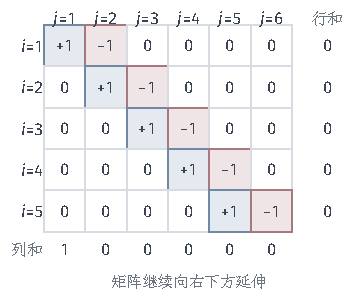
\includegraphics[width=59.951mm]{figures/02-abstract-mathematics/01-metric-and-measure/tikz/c3-fubini-counterexample/figure.pdf}
\caption{无穷矩阵$a_{i,j}=\mathbf 1\{j=i\}-\mathbf 1\{j=i+1\}$的左上角五行六列，矩阵向右下方继续。蓝色单元为$+1$，红色单元为$-1$；每一整行的和为$0$，第一整列的和为$1$，其余整列的和为$0$（第六列的$+1$位于第六行，在图外）。}
\label{fig:integral-fubini-counterexample}
\end{figure}

连续函数也会出现同样的现象。在$(0,1)^2$上取
\[
 f(x,y)=\frac{x^2-y^2}{(x^2+y^2)^2}.
\]
直接求导得$\partial_y\bigl(y/(x^2+y^2)\bigr)=(x^2-y^2)/(x^2+y^2)^2=f(x,y)$，所以固定$x\in(0,1)$时
\[
 \int_0^1f(x,y)\,\mathrm dy=\Bigl[\frac{y}{x^2+y^2}\Bigr]_{y=0}^{y=1}=\frac1{1+x^2},
 \qquad
 \int_0^1\frac{\mathrm dx}{1+x^2}=\frac\pi4.
\]
由于$f(y,x)=-f(x,y)$，先对$x$积分的内层结果是$-1/(1+y^2)$，这一次序得到$-\pi/4$。两种次序的结果都有限却不相等，原因仍是绝对可积性失效。在$0<y<x$处$f>0$，因此
\[
 \int_0^1|f(x,y)|\,\mathrm dy\ge\int_0^xf(x,y)\,\mathrm dy=\Bigl[\frac{y}{x^2+y^2}\Bigr]_{y=0}^{y=x}=\frac1{2x},
\]
而$\int_0^1(2x)^{-1}\,\mathrm dx=\infty$，由Tonelli定理，$\int_{(0,1)^2}|f|\,\mathrm d\lambda_2=\infty$。用极坐标看，$|f|=|\cos2\theta|/r^2$，面积元带一个$r$，原点附近的径向积分$\int_0^1r^{-1}\,\mathrm dr$发散；正、负两部分在原点附近各自累计出无穷，先积哪个变量决定了两者怎样相减。

\subsection{多重积分与截面计算}
\label{sec:integral-multiple}

\paragraph{有限乘积与Lebesgue测度}
三个或更多因子的乘积可以逐次组成。对$\sigma$有限测度空间$(X_k,\mathcal A_k,\mu_k)$（$k=1,2,3$），$(\mathcal A_1\otimes\mathcal A_2)\otimes\mathcal A_3$与$\mathcal A_1\otimes(\mathcal A_2\otimes\mathcal A_3)$都由“三重矩形”$A_1\times A_2\times A_3$生成，因而相同；两种组合方式得到的乘积测度在三重矩形上都等于$\mu_1(A_1)\mu_2(A_2)\mu_3(A_3)$，三重矩形是对有限交封闭且可被有限测度者可数覆盖的生成族，由唯一性它们相同。因此$\mu_1\otimes\cdots\otimes\mu_d$与组合括号无关，反复使用Tonelli或Fubini定理，非负或绝对可积的多重积分可以按任意坐标次序逐次计算。无限多个坐标的乘积以及随机过程分布的构造需要另外的工具，留给概率空间与随机过程的相关部分。

剩下要核对的是，第二章用轴平行矩形直接构造的$d$维Lebesgue测度$\lambda_d$与逐次乘积是否相同（第~\ref{sec:measure-construction}节）。

\begin{theorem}[Lebesgue测度与乘积测度相容]
\label{thm:integral-lebesgue-product}
对$p,q\ge1$，$\mathcal B(\mathbb R^p)\otimes\mathcal B(\mathbb R^q)=\mathcal B(\mathbb R^{p+q})$，并且在这个$\sigma$代数上$\lambda_{p+q}=\lambda_p\otimes\lambda_q$。特别地，$\lambda_d$在Borel集上等于$d$个一维Lebesgue测度的乘积。
\end{theorem}

\begin{proof}
$\mathbb R^{p+q}$中的开集是可数个有理端点开盒之并，每个开盒是$\mathbb R^p$与$\mathbb R^q$中开盒的乘积，属于$\mathcal B(\mathbb R^p)\otimes\mathcal B(\mathbb R^q)$，故右侧的Borel $\sigma$代数包含在左侧。反过来，固定$B\in\mathcal B(\mathbb R^q)$，投影$(\bm x,\bm y)\mapsto\bm x$连续，$A\times\mathbb R^q$是Borel集$A$在连续映射下的原像，因此对Borel集$A$是Borel集；同理$\mathbb R^p\times B$是Borel集，两者之交$A\times B$也是，故左侧包含在右侧。

两测度在形如$\prod_{k=1}^{p+q}(a_k,b_k]$的有界半开盒上都等于各边长之积：在乘积一侧，这样的盒是$\mathbb R^p$与$\mathbb R^q$中两个半开盒的乘积。这些盒对有限交封闭（交集仍是半开盒或空集），生成$\mathcal B(\mathbb R^{p+q})$，并且可数个盒$[-n,n]^{p+q}$覆盖全空间且测度有限。由唯一性定理，两测度在Borel集上相同。
\end{proof}

$\lambda_d$定义在Lebesgue可测集$\mathcal L(\mathbb R^d)$上，它是Borel测度的完备化（第~\ref{sec:measure-construction}节），所以$(\mathbb R^{p+q},\mathcal L(\mathbb R^{p+q}),\lambda_{p+q})$是$\lambda_p\otimes\lambda_q$的完备化。对Lebesgue可测函数使用累次积分时，应采用上一小节的“几乎每个截面”版本。卷一用Riemann和建立了长方体和简单区域上的累次积分，被积函数通常连续，可参考\BookChapterRef{chap:multivariate-integration}{卷一“多元函数积分”章}；在那里成立的计算，在连续函数于有界闭区域上绝对可积的条件下，就是这里Fubini定理的特例，而Tonelli与Fubini定理还覆盖了无界区域、不连续函数和一般测度。

\paragraph{区域积分与切片}
对可测区域$E\subseteq X\times Y$，区域上的积分定义为$\int_Ef\,\mathrm d(\mu\otimes\nu)=\int f\mathbf 1_E\,\mathrm d(\mu\otimes\nu)$。函数$f\mathbf 1_E$的截面在$E_x$之外取零，于是在相应条件下
\[
 \int_Ef\,\mathrm d(\mu\otimes\nu)=\int_X\Bigl(\int_{E_x}f(x,y)\,\mathrm d\nu(y)\Bigr)\mathrm d\mu(x).
\]
内层积分的范围就是截面$E_x$；交换次序时，要按另一个方向重新读出截面$E^y$，而不是只交换微分记号。

\begin{example}[换序计算含$e^{y^2}$的累次积分]
\label{ex:integral-order-swap}
考虑$\int_0^1\bigl(\int_x^1e^{y^2}\,\mathrm dy\bigr)\mathrm dx$。内层的$e^{y^2}$没有初等原函数，按原次序无法直接用原函数计算。积分区域是三角形$E=\{(x,y):0\le x\le y\le1\}$，被积函数非负，Tonelli定理允许换序；$E$在固定$y$处的截面是$E^y=[0,y]$，所以
\[
 \int_0^1\Bigl(\int_0^ye^{y^2}\,\mathrm dx\Bigr)\mathrm dy=\int_0^1ye^{y^2}\,\mathrm dy=\frac{e-1}2.
\]
内层对$x$积分时$e^{y^2}$是常数，只产生截面长度$y$，而这个因子恰好使外层有原函数$\frac12e^{y^2}$。
\end{example}

\paragraph{层饼公式}
截面方法还能把一个积分改写成“按高度分层”的累计。设$(X,\mathcal A,\mu)$$\sigma$有限，$f:X\to[0,\infty]$可测，考察图像下方的区域
\[
 \Gamma=\{(x,t)\in X\times(0,\infty):0<t<f(x)\}.
\]
若$0<t<f(x)$，可以取有理数$r$使$t<r<f(x)$，所以$\Gamma=\bigcup_{r\in\mathbb Q,\,r>0}\bigl(\{f>r\}\times(0,r)\bigr)$，是可数个可测矩形之并，属于$\mathcal A\otimes\mathcal B(\mathbb R)$。对$\mathbf 1_\Gamma$用Tonelli定理计算$(\mu\otimes\lambda)(\Gamma)$的两种次序。

\begin{theorem}[层饼公式]
\label{thm:integral-layer-cake}
设$(X,\mathcal A,\mu)$是$\sigma$有限测度空间，$f:X\to[0,\infty]$可测。则
\begin{equation}
 \int_Xf\,\mathrm d\mu=\int_0^\infty\mu(\{f>t\})\,\mathrm dt,
 \label{eq:integral-layer-cake}
\end{equation}
两侧可以同为$+\infty$。
\end{theorem}

\begin{proof}
固定$x$，$\Gamma_x=(0,f(x))$，长度为$f(x)$（$f(x)=\infty$时为$\infty$），先对$t$累计得$\int_Xf\,\mathrm d\mu$。固定$t>0$，$\Gamma^t=\{x:f(x)>t\}$，先对$x$累计得$\int_0^\infty\mu(\{f>t\})\,\mathrm dt$。两者都等于$(\mu\otimes\lambda)(\Gamma)$。
\end{proof}

这个结果称为\term{层饼公式}（layer cake formula）。图~\ref{fig:integral-layer-cake}画出了$f(x)=e^{-x}$（$x\ge0$）的两种切法：(a)竖切得到的长度是函数值，(b)横切得到的是超水平集$\{f>t\}$。对这个函数，$t\in(0,1)$时$\{f>t\}=[0,-\ln t)$，$t\ge1$时为空集，所以右侧为$\int_0^1(-\ln t)\,\mathrm dt=\bigl[t-t\ln t\bigr]_0^1=1$，与$\int_0^\infty e^{-x}\,\mathrm dx=1$一致。公式的价值在于右侧只需要知道各高度以上的集合有多大，不必知道这些集合在$X$中的位置；这也是第~\ref{sec:integral-definition}节按取值分层逼近函数的思路。

\begin{figure}[!htbp]
\centering
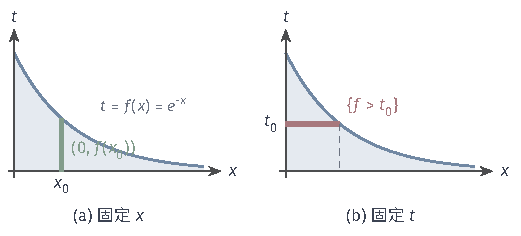
\includegraphics[width=88.149mm]{figures/02-abstract-mathematics/01-metric-and-measure/tikz/c3-layer-cake/figure.pdf}
\caption{层饼公式的两种切法，$f(x)=e^{-x}$，纵轴放大两倍绘制。(a)固定$x_0=0.8$，竖直截面是$(0,f(x_0))$，长度$e^{-0.8}\approx0.449$；(b)固定$t_0=0.4$，水平截面是$\{f>t_0\}=[0,-\ln0.4)\approx[0,0.916)$。两种截面长度分别对$x$和对$t$累计，都得到阴影区域的面积$1$。}
\label{fig:integral-layer-cake}
\end{figure}

\section{积分换元}
\label{sec:integral-change-of-variables}

累次积分保留原来的坐标，只改变累计次序。换元则通过一个映射把积分搬到另一个空间：对输出空间上的函数求积分，能否改成对输入空间上的复合函数求积分？本节按映射所满足的条件逐层具体化。一般可测映射只携带测度，换元规则由第二章的推前测度给出；若映射是欧氏空间开集间的光滑可逆变换，输出测度可以用Jacobian行列式写成Lebesgue测度的加权形式；若映射只能分成若干可逆分支，就逐支换元再累计。这里的“换元”始终是两个空间之间的变量替换；第四章在同一空间上更换参考测度，那是另一种运算。

\subsection{可测映射下的换元}
\label{sec:integral-pushforward-change}

设$T:(X,\mathcal A)\to(Y,\mathcal B)$可测，$\mu$是$X$上的测度。第二章定义的推前测度（定义~\ref{def:measure-pushforward}）为$(T_\#\mu)(B)=\mu(T^{-1}(B))$：目标集合$B$得到的质量，是落进$B$的那些输入点的质量。现在要问，对$Y$上的函数$h$，积分$\int_Yh\,\mathrm d(T_\#\mu)$怎样回到输入空间计算。

先看示性函数$h=\mathbf 1_B$。左侧是$(T_\#\mu)(B)=\mu(T^{-1}(B))$；而$\mathbf 1_B(T(x))=1$当且仅当$x\in T^{-1}(B)$，所以$\mathbf 1_B\circ T=\mathbf 1_{T^{-1}(B)}$，右侧$\int_X\mathbf 1_B\circ T\,\mathrm d\mu$也等于$\mu(T^{-1}(B))$。沿积分的构造步骤推广，就得到一般结论。

\begin{theorem}[推前测度的积分换元]
\label{thm:integral-pushforward-change}
设$(X,\mathcal A,\mu)$是测度空间，$T:X\to Y$是$(\mathcal A,\mathcal B)$可测映射。
\begin{enumerate}
 \item 对每个可测$h:Y\to[0,\infty]$，
 \begin{equation}
  \int_Yh\,\mathrm d(T_\#\mu)=\int_Xh\circ T\,\mathrm d\mu,
  \label{eq:integral-pushforward-change}
 \end{equation}
 两侧可以同为$+\infty$。
 \item 对可测的实值或复值$h$，$h$关于$T_\#\mu$可积当且仅当$h\circ T$关于$\mu$可积，此时式~\eqref{eq:integral-pushforward-change}成立且两侧有限。
\end{enumerate}
\end{theorem}

\begin{proof}
$h\circ T$是可测映射的复合，因而可测（第~\ref{sec:measure-measurable-maps}节）。(1)示性函数的情形已在上面核对。对非负简单函数$s=\sum_ic_i\mathbf 1_{B_i}$，$s\circ T=\sum_ic_i\mathbf 1_{B_i}\circ T$，两侧由线性性相等。对一般非负可测$h$，取简单函数$s_n\uparrow h$，则$s_n\circ T\uparrow h\circ T$，两侧分别用单调收敛定理取极限。

(2)由$|h\circ T|=|h|\circ T$，把(1)用于$|h|$，两侧绝对积分相等，可积性等价。实值时$(h\circ T)^\pm=h^\pm\circ T$，对正部和负部分别用(1)后相减；复值时对实部和虚部分别处理。
\end{proof}

定理不要求$T$可逆、可微，甚至不要求两端有距离；它只用到可测性和推前测度的定义。式~\eqref{eq:integral-pushforward-change}可以从两个方向读：已知$\mu$时，用它计算输出空间上的积分；已知输出测度时，用它说明对复合函数$h\circ T$的累计只取决于$T$把质量送到了哪里。

\begin{example}[有限集合上的分组汇总]
\label{ex:integral-pushforward-finite}
取$X=\{1,2,3,4\}$，$\mu(\{k\})=k/10$；$Y=\{0,1\}$，$T(1)=T(3)=1$、$T(2)=T(4)=0$。输出点$0$的原像是$\{2,4\}$，所以$(T_\#\mu)(\{0\})=0.2+0.4=0.6$；同理$(T_\#\mu)(\{1\})=0.1+0.3=0.4$。取$h(0)=5$、$h(1)=2$，左侧是$5\times0.6+2\times0.4=3.8$；右侧逐个输入点计算$h(T(k))\mu(\{k\})$，得$2\times0.1+5\times0.2+2\times0.3+5\times0.4=3.8$。
\end{example}

图~\ref{fig:integral-pushforward-change}显示了两种算法的差别：右侧逐点累计，左侧先把映到同一输出点的输入质量合并，再乘以该点的函数值。多对一映射正是通过这种合并，把不同输入点的质量汇集到同一个输出点；整个计算没有用到任何“输出密度”，输出测度本身就是两个原子。

\begin{figure}[!htbp]
\centering
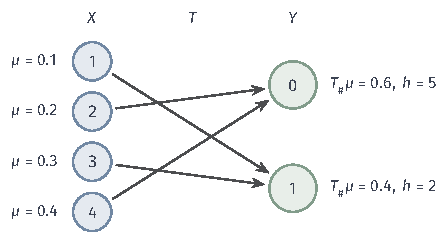
\includegraphics[width=75.812mm]{figures/02-abstract-mathematics/01-metric-and-measure/tikz/c3-pushforward-change/figure.pdf}
\caption{有限集合上的推前与换元。输入点$k=1,2,3,4$的质量为$k/10$，映射$T$把$2,4$送到$0$、把$1,3$送到$1$，输出质量分别为$0.6$与$0.4$。取$h(0)=5$、$h(1)=2$，按输出点汇总与按输入点逐个累计都得到$3.8$。}
\label{fig:integral-pushforward-change}
\end{figure}

由$(S\circ T)^{-1}(C)=T^{-1}(S^{-1}(C))$，推前满足$(S\circ T)_\#\mu=S_\#(T_\#\mu)$（第~\ref{sec:measure-pushforward}节），所以接连两次换元等于用复合映射一次换元，式~\eqref{eq:integral-pushforward-change}可以逐级使用。

\subsection{可逆光滑变换下的换元}
\label{sec:integral-jacobian-change}

当$X,Y$都是$\mathbb R^d$中的开集、$\mu=\lambda_d$时，定理~\ref{thm:integral-pushforward-change}把$\int h\circ T\,\mathrm d\lambda_d$转化为对推前测度$T_\#\lambda_d$的积分，但还没有说$T_\#\lambda_d$长什么样。若$T$光滑可逆，局部看来它近似一个线性变换，体积按一个确定的比例改变，这个比例就是Jacobian行列式的绝对值。

\paragraph{Jacobian换元公式}
设$U,V\subseteq\mathbb R^d$为开集。若$T:U\to V$是双射，$T$与$T^{-1}$都连续可微，则称$T$为\term{微分同胚}（diffeomorphism），更准确地说是$C^1$微分同胚。对$T^{-1}\circ T=\mathrm{id}$求导得$DT^{-1}(T(\bm x))DT(\bm x)=\bm I$，所以$\det DT(\bm x)\ne0$处处成立；$\det DT$称为$T$的\term{Jacobian行列式}（Jacobian determinant）。卷一在多元积分一章对紧Jordan区域上的连续函数证明了经典换元公式：若$E\subseteq U$是紧Jordan区域且$T(E)$也是Jordan区域，$f$在$T(E)$上连续，则$\int_{T(E)}f(\bm y)\,\mathrm d\bm y=\int_Ef(T(\bm x))|\det DT(\bm x)|\,\mathrm d\bm x$。现在把它推广到一般可测函数。

\begin{theorem}[可逆光滑变换下的换元]
\label{thm:integral-jacobian-change}
设$U,V\subseteq\mathbb R^d$为开集，$T:U\to V$是$C^1$微分同胚。对每个Lebesgue可测$h:V\to[0,\infty]$，
\begin{equation}
 \int_Vh(\bm y)\,\mathrm d\bm y=\int_Uh(T(\bm x))\,|\det DT(\bm x)|\,\mathrm d\bm x,
 \label{eq:integral-jacobian-change}
\end{equation}
两侧可以同为$+\infty$。若$h$是实值或复值Lebesgue可测函数，则$h$在$V$上可积当且仅当$(h\circ T)|\det DT|$在$U$上可积，此时式~\eqref{eq:integral-jacobian-change}成立且两侧有限。
\end{theorem}

\begin{proof}
论证的任务是把经典公式中的“连续函数、Jordan区域”换成“可测函数、可测集合”。分四步进行。

第一步，构造比较对象。对Borel集$B\subseteq V$，令
\[
 \rho(B)=\int_U\mathbf 1_B(T(\bm x))\,|\det DT(\bm x)|\,\mathrm d\bm x.
\]
$T$连续，$\mathbf 1_B\circ T$是Borel函数；$|\det DT|$连续，因而可测。若$B_n$两两不交，$\mathbf 1_{\bigcup_nB_n}\circ T=\sum_n\mathbf 1_{B_n}\circ T$，非负级数可以逐项积分，所以$\rho$是$V$的Borel集上的测度。式~\eqref{eq:integral-jacobian-change}对示性函数说的正是$\rho=\lambda_d$。

第二步，在闭盒上比较。设$Q\subseteq V$是闭盒（允许退化）。$E=T^{-1}(Q)$是紧集，因为$T^{-1}$连续；$T^{-1}$是同胚，所以$E$的边界是$T^{-1}(\partial Q)$。$\partial Q$的Jordan容量为零，$T^{-1}$在$Q$的一个紧邻域上Lipschitz，把容量为零的集合映成容量为零的集合，故$E$是紧Jordan区域。对$f\equiv1$应用经典公式，得$\lambda_d(Q)=\int_E|\det DT|\,\mathrm d\bm x=\rho(Q)$；这里Jordan区域上连续函数的Riemann积分等于Lebesgue积分（第~\ref{sec:integral-classical}节）。

第三步，推广到Borel集与非负Borel函数。含于$V$的闭盒对有限交封闭（交集是闭盒或空集），$V$的每个开子集都是可数个含于其中的有理端点闭盒之并，所以它们生成$V$上的Borel $\sigma$代数，并且可数个这样的闭盒覆盖$V$，各自测度有限。由$\pi$--$\lambda$唯一性（定理~\ref{thm:measure-pi-lambda}），$\rho=\lambda_d$在$V$的Borel集上成立。由线性性，式~\eqref{eq:integral-jacobian-change}对非负Borel简单函数成立；取递增逼近并在两侧用单调收敛定理，它对非负Borel函数成立。

第四步，推广到Lebesgue可测函数。Lebesgue可测结构是Borel测度的完备化，因此非负Lebesgue可测$h$与某个非负Borel函数$\tilde h$只在一个Borel零测集$N\subseteq V$内不同。对$\mathbf 1_N$用第三步，$\int_U\mathbf 1_N(T(\bm x))|\det DT(\bm x)|\,\mathrm d\bm x=\lambda_d(N)=0$；被积函数非负、积分为零，所以它几乎处处为零，又因$|\det DT|>0$，得$\lambda_d(T^{-1}(N))=0$。于是$h\circ T$与$\tilde h\circ T$只在零测集上不同，前者Lebesgue可测，并且两侧积分分别与$\tilde h$的相应积分相同。实值或复值情形先对$|h|$使用非负结论确认可积性等价，再对正负部或实部、虚部分别使用。
\end{proof}

定理中的条件分别承担不同的任务：$C^1$保证局部体积比例由$|\det DT|$连续地描述，双射保证每块输出区域只被一个输入区域覆盖一次。若在正测度的区域上发生重叠，单一的换元公式会少算或多算质量，这是下一小节的问题。

\paragraph{线性变换与体积比例}
最简单的情形是仿射变换$T(\bm x)=\bm A\bm x+\bm b$，其中$\bm A$为可逆$d\times d$矩阵。此时$DT\equiv\bm A$，Jacobian因子是常数$|\det\bm A|$。对可测集$E\subseteq\mathbb R^d$，在式~\eqref{eq:integral-jacobian-change}中取$h=\mathbf 1_{T(E)}$，左侧是$\lambda_d(T(E))$，右侧是$\int_E|\det\bm A|\,\mathrm d\bm x$，于是
\[
 \lambda_d(\bm AE+\bm b)=|\det\bm A|\,\lambda_d(E).
\]
线性变换的行列式绝对值是固定的体积比例，平移的比例为$1$。图~\ref{fig:integral-jacobian-cell}中$\bm A=\begin{bmatrix}1.5&0.5\\0.5&1\end{bmatrix}$把单位正方形变成以两列为边的平行四边形，面积$|1.5\times1-0.5\times0.5|=1.25$；取绝对值是因为反射等改变定向的变换行列式为负，而面积非负。对一般的$C^1$微分同胚，$\bm x$附近的小块被近似地按$DT(\bm x)$线性变换，$|\det DT(\bm x)|$就是这一点处的局部体积比例。

\begin{figure}[!htbp]
\centering
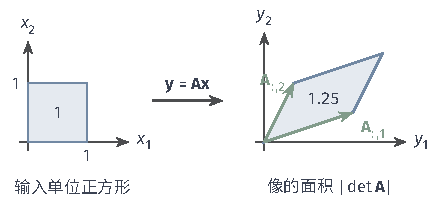
\includegraphics[width=74.701mm]{figures/02-abstract-mathematics/01-metric-and-measure/tikz/c3-jacobian-cell/figure.pdf}
\caption{可逆线性变换的体积比例。$\bm A=\begin{bmatrix}1.5&0.5\\0.5&1\end{bmatrix}$把面积为$1$的单位正方形映成以列向量$\bm A_{:,1}=(1.5,0.5)^\top$、$\bm A_{:,2}=(0.5,1)^\top$为边的平行四边形，面积为$|\det\bm A|=1.25$。}
\label{fig:integral-jacobian-cell}
\end{figure}

\begin{example}[极坐标与Gauss积分]
\label{ex:integral-polar-gauss}
令$U=(0,\infty)\times(0,2\pi)$，$T(r,\theta)=(r\cos\theta,r\sin\theta)$，$V=\mathbb R^2\setminus\{(x,0):x\ge0\}$。$T:U\to V$是$C^1$微分同胚，$\det DT(r,\theta)=r$。被去掉的射线是$\lambda_2$零测集（它包含在矩形$[0,\infty)\times\{0\}$中，测度为$\infty\cdot0=0$），不影响积分。取$h(x,y)=e^{-(x^2+y^2)}$，
\[
 \int_{\mathbb R^2}e^{-(x^2+y^2)}\,\mathrm d\lambda_2=\int_0^{2\pi}\!\!\int_0^\infty e^{-r^2}r\,\mathrm dr\,\mathrm d\theta=2\pi\cdot\frac12=\pi,
\]
右侧的累次积分由Tonelli定理得到。另一方面，左侧的被积函数是$e^{-x^2}e^{-y^2}$，Tonelli定理给出它等于$\bigl(\int_{\mathbb R}e^{-x^2}\,\mathrm dx\bigr)^2$，于是$\int_{\mathbb R}e^{-x^2}\,\mathrm dx=\sqrt\pi$。
\end{example}

Jacobian公式只是在通用换元关系~\eqref{eq:integral-pushforward-change}的基础上，对可逆光滑变换进一步识别了体积如何变化。一般可测映射不满足它的条件：$T$不可逆时输出可能重叠，$T$把$\mathbb R^d$映到低维集合时输出集合的$d$维体积为零。后一种情形需要曲线、曲面上的面积测度或余面积公式，留给相应的几何内容。

\subsection{分支可逆变换下的换元}
\label{sec:integral-branch-change}

许多常用变换不是整体可逆的，但可以分成几段，每段可逆。例如$T(x)=x^2$在$(-1,1)$上把$x$与$-x$送到同一点，在$(0,1)$和$(-1,0)$上却分别是微分同胚。对这类映射，把输入区域分开，逐支应用上一小节的定理，再把结果加起来。

\begin{theorem}[分支可逆变换下的换元]
\label{thm:integral-branch-change}
设$U\subseteq\mathbb R^d$为开集，$N\subseteq U$是Lebesgue零测集，$U\setminus N$是有限或可数个两两不交开集$U_k$之并；设$T:U\to\mathbb R^d$在每个$U_k$上的限制$T_k:U_k\to V_k=T(U_k)$都是开集之间的$C^1$微分同胚。则对每个Lebesgue可测$f:U\to[0,\infty]$，
\begin{equation}
 \int_Uf(\bm x)\,\mathrm d\bm x=\sum_k\int_{V_k}f\bigl(T_k^{-1}(\bm y)\bigr)\,\bigl|\det DT_k^{-1}(\bm y)\bigr|\,\mathrm d\bm y.
 \label{eq:integral-branch-change}
\end{equation}
若$f$是实值或复值可积函数，上式右侧的级数绝对收敛，等式仍成立。
\end{theorem}

\begin{proof}
零测集不影响积分，$\int_Uf=\int_{U\setminus N}f$。$U\setminus N$是两两不交的$U_k$之并，$f\mathbf 1_{U\setminus N}=\sum_kf\mathbf 1_{U_k}$，非负级数可以逐项积分，故$\int_Uf=\sum_k\int_{U_k}f$；可数个分支的累计正是由单调收敛保证的。对第$k$项，把定理~\ref{thm:integral-jacobian-change}用于微分同胚$T_k^{-1}:V_k\to U_k$和$U_k$上的函数$f$，得到
\[
 \int_{U_k}f(\bm x)\,\mathrm d\bm x=\int_{V_k}f\bigl(T_k^{-1}(\bm y)\bigr)\,\bigl|\det DT_k^{-1}(\bm y)\bigr|\,\mathrm d\bm y.
\]
相加即得式~\eqref{eq:integral-branch-change}。可积情形先对$|f|$使用非负结论，得到右侧绝对收敛，再对正负部或实部、虚部分别处理。
\end{proof}

式~\eqref{eq:integral-branch-change}右侧是对分支求和，不是在输出空间上选一个逆。各分支的像$V_k$可以重叠：若某点$\bm y$同时属于$V_1$和$V_2$，它有两个原像，两项都要计入；只选择一个逆分支，就会漏掉另一个原像那里的质量。把$f=h\circ T$代入就能看清这一点：
\[
 \int_Uh(T(\bm x))\,\mathrm d\bm x=\int h(\bm y)\sum_k\mathbf 1_{V_k}(\bm y)\,\bigl|\det DT_k^{-1}(\bm y)\bigr|\,\mathrm d\bm y,
\]
输出点$\bm y$的权重是它所有原像分支的体积比例之和。另一个条件是被扔掉的$N$必须零测。若某一部分输入区域没有纳入任何分支且测度为正，例如$T$在一段区间上取常值，那部分的积分要另外计算，不能直接删去；单个微分同胚的情形既没有重叠，也没有剩余部分，所以不需要这两项检查。

\begin{example}[平方映射的两个分支]
\label{ex:integral-square-branches}
取$U=(-1,1)$，$T(x)=x^2$，$N=\{0\}$，$U_1=(0,1)$、$U_2=(-1,0)$，两支的像都是$V_1=V_2=(0,1)$，如图~\ref{fig:integral-branch-inverse}。逆分支为$T_1^{-1}(y)=\sqrt y$与$T_2^{-1}(y)=-\sqrt y$，导数分别是$1/(2\sqrt y)$与$-1/(2\sqrt y)$，绝对值都是$1/(2\sqrt y)$。式~\eqref{eq:integral-branch-change}给出
\[
 \int_{-1}^1f(x)\,\mathrm dx=\int_0^1\frac{f(\sqrt y)+f(-\sqrt y)}{2\sqrt y}\,\mathrm dy.
\]
取$f\equiv1$，左侧为$2$，右侧为$\int_0^1y^{-1/2}\,\mathrm dy=\bigl[2\sqrt y\bigr]_0^1=2$。若只用一个逆分支，右侧只剩$1$，恰好漏掉$(-1,0)$上的质量。原点处导数为零，$T$在那里不是局部微分同胚，但$\{0\}$零测，把它放进$N$不影响结果。再取$f(x)=x^2$检验：左侧为$2/3$，右侧为$\int_0^1\frac{2y}{2\sqrt y}\,\mathrm dy=\int_0^1y^{1/2}\,\mathrm dy=2/3$。第四章还会用同一个变换计算输出测度的密度。
\end{example}

\begin{figure}[!htbp]
\centering
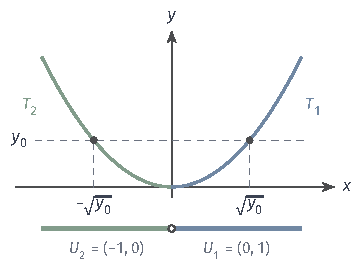
\includegraphics[width=61.33mm]{figures/02-abstract-mathematics/01-metric-and-measure/tikz/c3-branch-inverse/figure.pdf}
\caption{平方映射$T(x)=x^2$在$(-1,1)$上的两个可逆分支。蓝色分支$T_1$定义在$U_1=(0,1)$上，绿色分支$T_2$定义在$U_2=(-1,0)$上，空心点$x=0$是被去掉的零测集。水平线$y=y_0$与两个分支分别交于$\sqrt{y_0}$与$-\sqrt{y_0}$，所以每个输出值都要累计两个原像的贡献。}
\label{fig:integral-branch-inverse}
\end{figure}

\section{含参积分}
\label{sec:integral-parametric}

许多量是“对一个变量积分、随另一个变量变化”的函数。例如$F(t)=\int_0^\infty e^{-tx}\,\mathrm dx$随衰减率$t$变化，模型的平均损失随参数变化。设$(X,\mathcal A,\mu)$是测度空间，$I\subseteq\mathbb R$是区间，$f:I\times X\to\mathbb R$（或$\mathbb C$），并且对每个$t\in I$，截面$f(t,\cdot)$都是可测函数。只要积分有意义，就得到一元函数
\[
 F(t)=\int_Xf(t,x)\,\mathrm d\mu(x),
\]
称为\term{含参积分}（parameter-dependent integral）。测度和积分区域都固定不动，参数的变化完全体现在被积函数上。本节的问题是：$f$对$t$连续或可微时，$F$是否也连续或可微？参数的变化是一种极限过程，因此答案来自第~\ref{sec:integral-limits}节的控制收敛定理；关键是找到对一族参数同时有效的可积控制。

\subsection{积分关于参数的连续性}
\label{sec:integral-parametric-continuity}

对每个固定的$x$，$t\mapsto f(t,x)$连续，只说明每个位置上的取值连续变化。质量却可能随参数移向无穷远或集中到越来越小的区域，这在任何固定位置上都看不出来。用一个可积函数同时控制附近全部参数的被积函数，就排除了这两种可能。

\begin{theorem}[含参积分的连续性]
\label{thm:integral-parametric-continuity}
设$t_0\in I$，$J$是$t_0$在$I$中的一个邻域（相对于$I$），$g\ge0$关于$\mu$可积。若
\begin{enumerate}
 \item 对$\mu$-几乎所有$x$，$t\mapsto f(t,x)$在$t_0$处连续；
 \item 对每个$t\in J$，$|f(t,x)|\le g(x)$对$\mu$-几乎所有$x$成立，
\end{enumerate}
则对$t\in J$，$F(t)$有限，并且$F$在$t_0$处连续。
\end{theorem}

\begin{proof}
由条件(2)，每个$f(t,\cdot)$（$t\in J$）都被可积函数$g$控制，因而可积，$F(t)$有限。任取$J$中的序列$t_n\to t_0$。条件(1)的例外集是一个零测集；条件(2)对每个$t_n$和$t_0$各有一个零测例外集，可数个零测集之并仍零测。在这些例外集之外，$f(t_n,x)\to f(t_0,x)$且$|f(t_n,x)|\le g(x)$，控制收敛定理~\ref{thm:integral-dominated-convergence}给出$F(t_n)\to F(t_0)$。实变量函数的序列判据说明$F$在$t_0$连续。
\end{proof}

证明中合并例外集时只用到了可数个参数值，所以条件(2)的例外集可以随$t$改变；条件(1)的例外集则是对一个固定的$x$集合说的，不随参数变化。控制只需在所考察点的一个邻域内成立，不必用一个函数覆盖整个参数区间。

\begin{example}[局部控制与整体控制]
\label{ex:integral-parametric-local}
令$F(t)=\int_0^\infty e^{-tx}\,\mathrm dx=1/t$（$t>0$）。在$(0,\infty)$上找不到统一的控制：$\sup_{t>0}e^{-tx}=1$，常数$1$在$[0,\infty)$上不可积。但固定$t_0>0$，在邻域$J=(t_0/2,\infty)$上有$e^{-tx}\le e^{-t_0x/2}$，右侧可积，积分为$2/t_0$。定理给出$F$在$t_0$连续；$t_0$任意，所以$F$在整个$(0,\infty)$上连续。每个参数点各用自己的包络就够了。
\end{example}

\paragraph{控制失效的情形}
在参数区间的边界附近，局部控制可能不存在，此时结论也可能失效。在$[0,\infty)$上令$f(t,x)=te^{-tx}$（$t>0$），并按逐点极限补充$f(0,x)=0$。对每个$t>0$，
\[
 F(t)=\int_0^\infty te^{-tx}\,\mathrm dx=1,
\]
而$F(0)=0$，所以$F$在$t=0$处不连续，尽管对每个固定的$x$都有$f(t,x)\to0=f(0,x)$。图~\ref{fig:integral-parameter-continuity}显示了原因：$t$越小，曲线越低越平，同样为$1$的质量被推向越来越远的地方。由$\int_c^\infty te^{-tx}\,\mathrm dx=e^{-tc}$，一半质量位于$x\ge(\ln2)/t$处，这个位置随$t\downarrow0$趋于无穷。

任何控制函数都必须位于这族曲线的上包络之上。对$x>1/\delta$，函数$t\mapsto te^{-tx}$在$t=1/x\in(0,\delta)$处取最大值，所以
\[
 \sup_{0<t<\delta}te^{-tx}=\frac1{ex},
\]
它在$(1/\delta,\infty)$上不可积。于是$t=0$的任何邻域都没有可积控制，定理的条件不成立。这个例子提醒我们，结论只适用于已经核对了控制条件的参数范围。

\begin{figure}[!htbp]
\centering
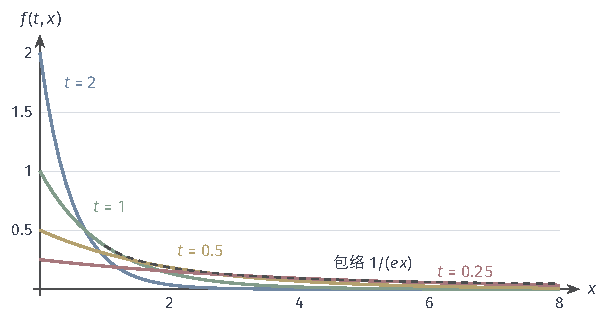
\includegraphics[width=102.807mm]{figures/02-abstract-mathematics/01-metric-and-measure/tikz/c3-parameter-continuity/figure.pdf}
\caption{含参积分中质量的逃逸。四条实线是$f(t,x)=te^{-tx}$在$t=2,1,0.5,0.25$时的图像，每条曲线下的面积都是$1$；$t$越小，质量越向右摊开。虚线是包络$\sup_tte^{-tx}=1/(ex)$（在$t=1/x$处取到，画在$x\ge1$部分），它在无穷远处不可积，所以$t=0$附近没有可积控制。}
\label{fig:integral-parameter-continuity}
\end{figure}

\subsection{积分号下求导}
\label{sec:integral-differentiate-under-sign}

若$f(t,x)$对$t$可微，自然希望$F'(t)=\int_X\partial_tf(t,x)\,\mathrm d\mu(x)$，即总量的变化率等于各处变化率的累计。这种运算称为\term{积分号下求导}（differentiation under the integral sign）。左侧是差商$\bigl(F(t+h)-F(t)\bigr)/h=\int_X\frac{f(t+h,x)-f(t,x)}{h}\,\mathrm d\mu(x)$在$h\to0$时的极限，所以这又是一次极限与积分的交换。控制的对象是差商；对实值函数，中值定理把差商的控制归结为偏导数的控制。

\begin{theorem}[积分号下求导]
\label{thm:integral-differentiate-under-integral}
设$J\subseteq I$是开区间，$f$为实值，$N\in\mathcal A$为$\mu$零测集，$g\ge0$关于$\mu$可积，且
\begin{enumerate}
 \item 对每个$x\notin N$，$t\mapsto f(t,x)$在$J$上可微，并且$|\partial_tf(t,x)|\le g(x)$对所有$t\in J$成立；
 \item 存在$t_1\in J$，使$f(t_1,\cdot)$关于$\mu$可积。
\end{enumerate}
则对每个$t\in J$，$f(t,\cdot)$可积，$F$在$J$上可微，并且
\begin{equation}
 F'(t)=\int_X\partial_tf(t,x)\,\mathrm d\mu(x),
 \label{eq:integral-differentiate-under-integral}
\end{equation}
其中$\partial_tf(t,\cdot)$在$N$上取值$0$。
\end{theorem}

\begin{proof}
对$x\notin N$与$t\in J$，中值定理给出$|f(t,x)-f(t_1,x)|\le|t-t_1|g(x)$，所以$|f(t,\cdot)|\le|f(t_1,\cdot)|+|t-t_1|g$几乎处处成立，右侧可积，$f(t,\cdot)$可积。

固定$t\in J$，任取非零序列$h_n\to0$且$t+h_n\in J$，令
\[
 q_n(x)=\frac{f(t+h_n,x)-f(t,x)}{h_n}.
\]
每个$q_n$是两个可测函数之差的倍数，因而可测。对$x\notin N$，$q_n(x)\to\partial_tf(t,x)$，所以$\partial_tf(t,\cdot)\mathbf 1_{X\setminus N}$是可测函数列$q_n\mathbf 1_{X\setminus N}$的逐点极限，它是可测的；这正是选择在$N$上取零的原因。中值定理又给出$|q_n(x)|\le g(x)$（$x\notin N$）。由控制收敛定理，
\[
 \frac{F(t+h_n)-F(t)}{h_n}=\int_Xq_n\,\mathrm d\mu\longrightarrow\int_X\partial_tf(t,x)\,\mathrm d\mu(x).
\]
序列$h_n$任意，由序列判据，$F$在$t$处可微且导数为式~\eqref{eq:integral-differentiate-under-integral}右侧。
\end{proof}

复值的$f$可以对实部和虚部分别使用定理。条件(1)中的零测集$N$和控制函数$g$都不能随参数改变：参数有不可数多个，各参数的例外集之并未必零测，也未必可测。这一组条件便于核对，但只是充分条件；更一般地，只需在$t$的邻域内用同一个可积函数控制全部差商。

\begin{example}[对$e^{-tx}$在积分号下逐阶求导]
\label{ex:integral-differentiate-exponential}
仍取$F(t)=\int_0^\infty e^{-tx}\,\mathrm dx=1/t$。固定$t_0>0$，取$J=(t_0/2,3t_0/2)$，则对$t\in J$，
\[
 |\partial_te^{-tx}|=xe^{-tx}\le xe^{-t_0x/2},
\]
右侧可积，分部积分得其积分为$4/t_0^2$。条件(2)由$F(t_0)$有限保证，例外集可取$N=\varnothing$。定理给出$F'(t_0)=-\int_0^\infty xe^{-t_0x}\,\mathrm dx$；与直接求导$F'(t_0)=-1/t_0^2$比较，得$\int_0^\infty xe^{-t_0x}\,\mathrm dx=1/t_0^2$。

高阶导数要逐阶重新核对。设已经得到
\[
 F^{(k)}(t)=(-1)^k\int_0^\infty x^ke^{-tx}\,\mathrm dx,
\]
则第$k+1$阶需要的控制是
\[
 |\partial_t(x^ke^{-tx})|=x^{k+1}e^{-tx}\le x^{k+1}e^{-t_0x/2}\qquad(t\in J),
\]
右侧可积，故可再求一次导。逐阶完成后与$\frac{\mathrm d^k}{\mathrm dt^k}t^{-1}=(-1)^kk!\,t^{-k-1}$比较，得到
\[
 \int_0^\infty x^ke^{-tx}\,\mathrm dx=\frac{k!}{t^{k+1}}\qquad(t>0,\ k=0,1,2,\ldots).
\]
每一阶用的都是$t_0$附近的局部控制；若参数范围包含任意接近零的正数，同一个包络就不再适用。
\end{example}

\paragraph{偏导存在不等于可以交换}
偏导数逐点存在并不足以交换求导与积分。对$x\in(0,1)$与$t\ge0$，令$f(t,x)=tx/(x^2+t^2)$（$t>0$），$f(0,x)=0$。在$t=0$处，对每个固定的$x$，差商$f(t,x)/t=x/(x^2+t^2)\to1/x$，所以右偏导数$\partial_tf(0,x)=1/x$处处存在，但$1/x$在$(0,1)$上不可积。另一方面，令$u=x^2+t^2$直接积分，
\[
 F(t)=\frac t2\ln\frac{1+t^2}{t^2}\quad(t>0),\qquad F(0)=0,
\]
所以$F(t)/t=\frac12\ln(1+t^{-2})\to\infty$（$t\downarrow0$），$F$在$0$处没有有限的右导数。差商$x/(x^2+t^2)$在$x=t$处等于$1/(2t)$，峰值随$t\downarrow0$无界地升高并移向原点，找不到统一的可积控制，交换就失效了。

\section{积分与微分}
\label{sec:integral-differentiation}

卷一的微积分基本定理有两个方向：被积函数$g$连续时，累计函数$G(x)=\int_a^xg(t)\,\mathrm dt$可导且$G'=g$；$F$连续可导时，$F(b)-F(a)=\int_a^bF'(t)\,\mathrm dt$（可参考\BookChapterRef{chap:univariate-integration}{卷一“一元函数的积分”章}）。有了Lebesgue积分，被积函数只需可积，导数也只需几乎处处存在，两个方向都要重新回答：可积函数的累计函数在什么意义下可导，导数是否回到原函数？哪些函数能由导数的积分恢复？第二章的Cantor函数连续、单调，导数几乎处处为零，整体却从$0$增到$1$，可见“连续且几乎处处可导”不够。本节回到有限闭区间$[a,b]$上的实值函数，先定义控制多个区间总增量的绝对连续性，再用有界变差和区间覆盖得到导数的存在与总量估计，然后分别处理积分函数的求导和由导数恢复函数，最后用Cantor函数检查恢复公式的边界。全部论证只用一元函数和区间覆盖，不使用第四章的相对密度。

\subsection{绝对连续函数}
\label{sec:integral-absolutely-continuous}

\paragraph{从单个区间到多个区间}
一致连续要求：只要一个区间足够短，函数在它两端的增量就小。要由导数恢复增量，这还不够，因为导数为零的地方可能散布着许多极短的区间，函数恰好在这些区间上完成全部增长。需要控制的是许多互不相交的小区间上的总增量。

\begin{definition}[绝对连续函数]
\label{def:integral-absolutely-continuous-function}
设$F:[a,b]\to\mathbb R$。若对任意$\varepsilon>0$存在$\delta>0$，使得对$[a,b]$中任意有限个两两不交的开区间$(a_1,b_1),\ldots,(a_m,b_m)$，只要$\sum_{i=1}^m(b_i-a_i)<\delta$，就有
\[
 \sum_{i=1}^m|F(b_i)-F(a_i)|<\varepsilon,
\]
则称$F$在$[a,b]$上绝对连续，也称$F$是$[a,b]$上的\term{绝对连续函数}（absolutely continuous function）。
\end{definition}

取$m=1$就回到一致连续的要求，所以绝对连续函数一致连续。区别在于$\delta$必须对任意多个小区间同时有效：区间个数不受限制，只限制总长度。图~\ref{fig:integral-absolute-continuity-intervals}中取$F(x)=\sqrt x$，横轴上四段绿色区间总长$1.2$，纵轴上对应的四段红色增量总和约为$0.562$；绝对连续性要求，当绿色总长趋于零时，红色总和也一致地趋于零，无论区间怎样分布、分成多少段。

\begin{figure}[!htbp]
\centering
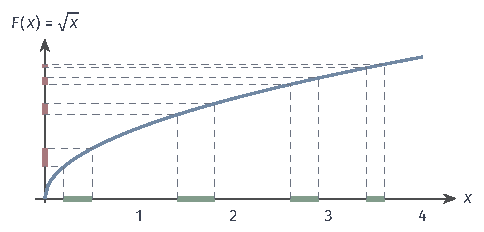
\includegraphics[width=81.933mm]{figures/02-abstract-mathematics/01-metric-and-measure/tikz/c3-absolute-continuity-intervals/figure.pdf}
\caption{绝对连续性控制的是多个不交区间上的总增量。$F(x)=\sqrt x$，纵轴放大$1.2$倍绘制。横轴上的绿色区间为$(0.2,0.5)$、$(1.4,1.8)$、$(2.6,2.9)$、$(3.4,3.6)$，总长$1.2$；纵轴上的红色线段是相应增量$0.260$、$0.158$、$0.090$、$0.053$，总和约为$0.562$。靠近原点的区间虽短，增量却最大。}
\label{fig:integral-absolute-continuity-intervals}
\end{figure}

\paragraph{基本例子与性质}
若$F$满足Lipschitz条件$|F(x)-F(y)|\le L|x-y|$，则$\sum_i|F(b_i)-F(a_i)|\le L\sum_i(b_i-a_i)$，取$\delta=\varepsilon/L$即可，所以Lipschitz函数绝对连续；特别地，$[a,b]$上连续可导的函数由中值定理满足Lipschitz条件，因而绝对连续。有限线性组合保持绝对连续：若$F,G$绝对连续、$\alpha,\beta\in\mathbb R$，对$\varepsilon$分别取$F,G$的$\delta_F,\delta_G$，使对应总增量小于$\varepsilon/(2|\alpha|+2|\beta|+1)$，令$\delta=\min(\delta_F,\delta_G)$，三角不等式给出$\alpha F+\beta G$的总增量小于$\varepsilon$。绝对连续函数不一定Lipschitz：$\sqrt x$在$[0,4]$上于原点附近斜率无界，却绝对连续，这一点在第~\ref{sec:integral-indefinite}小节可以直接看出。

这里的“绝对连续”描述的是函数增量受区间长度的控制，与第二章两个测度之间的绝对连续$\nu\ll\mu$（定义~\ref{def:measure-absolutely-continuous}）定义不同。两者怎样通过函数增量所确定的测度联系起来，留到第四章的密度计算中说明。

\subsection{有界变差与几乎处处可导}
\label{sec:integral-bounded-variation}

\paragraph{全变差}
要从导数读出函数的变化，先要确认变化的总量有限。

\begin{definition}[有界变差函数]
\label{def:integral-bounded-variation}
对$F:[a,b]\to\mathbb R$和$[a,b]$的分割$P:a=x_0<x_1<\cdots<x_n=b$，令$V(F,P)=\sum_{k=1}^n|F(x_k)-F(x_{k-1})|$。称
\[
 V_a^b(F)=\sup_PV(F,P)
\]
为$F$在$[a,b]$上的\term{全变差}（total variation）。若$V_a^b(F)<\infty$，称$F$为$[a,b]$上的\term{有界变差函数}（function of bounded variation）。
\end{definition}

函数的全变差是沿区间累计的增量绝对值，与第二章有符号测度的总变差测度$|\nu|$是不同的对象。单调函数的全变差就是端点增量$|F(b)-F(a)|$，因为每个分割上的和都可以伸缩相消。全变差对区间可加：若$a<c<b$，则$V_a^b(F)=V_a^c(F)+V_c^b(F)$。理由是在分割中插入点$c$不会减小$V(F,P)$（三角不等式），而插入$c$后的分割恰好分成$[a,c]$与$[c,b]$两部分的分割。

\begin{lemma}[绝对连续函数有界变差]
\label{lem:integral-ac-bv}
若$F$在$[a,b]$上绝对连续，则$F$是有界变差函数。
\end{lemma}

\begin{proof}
对$\varepsilon=1$取定义中的$\delta$。把$[a,b]$等分成$K$段，$K$取得足够大使每段长度小于$\delta$。在一段$[c,d]$内任取分割，其小区间两两不交、总长小于$\delta$，增量之和小于$1$，故$V_c^d(F)\le1$。由区间可加性，$V_a^b(F)\le K$。
\end{proof}

一致连续不能推出有界变差。在$[0,1]$上令$F(x)=x\sin(1/x)$（$x>0$）、$F(0)=0$，它在紧区间上连续，因而一致连续。取$x_k=1/((k+\frac12)\pi)$，则$F(x_k)=(-1)^kx_k$，相邻两点的增量绝对值为$x_k+x_{k+1}>x_k$，于是$V_0^1(F)\ge\sum_kx_k=\sum_k\frac1{(k+\frac12)\pi}=\infty$。由引理~\ref{lem:integral-ac-bv}，这个函数也不绝对连续。

有界变差函数总能写成两个单调函数之差。令$V(x)=V_a^x(F)$（$V(a)=0$），称为$F$的\term{变差函数}（variation function）。对$a\le x<y\le b$，由区间可加性，$V(y)-V(x)=V_x^y(F)\ge|F(y)-F(x)|$。因此$V$与$V-F$都单调不减，且
\[
 F=V-(V-F)
\]
是两个有限值单调不减函数之差。这一分解只用到函数本身，没有构造任何测度；它把有界变差函数的研究归结为单调函数。

\paragraph{单调函数的可导性}
单调函数可能在可数个点跳跃，也可能像Cantor函数那样在零测集上完成增长，但它在几乎每一点都有有限导数。证明的核心是一个区间选择引理。设$E\subseteq\mathbb R$，$\mathcal V$是一族非退化闭区间；若对每个$x\in E$和每个$\eta>0$，都有$I\in\mathcal V$满足$x\in I$且$|I|<\eta$，就称$\mathcal V$为$E$的\term{Vitali覆盖}（Vitali cover），其中$|I|$表示区间长度。

\begin{lemma}[Vitali覆盖引理]
\label{lem:integral-vitali}
设$E\subseteq\mathbb R$的外测度$\lambda^*(E)<\infty$，$\mathcal V$是$E$的Vitali覆盖。则对任意$\varepsilon>0$，存在$\mathcal V$中有限个两两不交的区间$I_1,\ldots,I_N$，使$\lambda^*\bigl(E\setminus\bigcup_{k=1}^NI_k\bigr)<\varepsilon$。
\end{lemma}

\begin{proof}
由外测度的定义（定义~\ref{def:measure-outer}），可以用可数个开区间覆盖$E$且总长不超过$\lambda^*(E)+1$，它们的并是开集$O\supseteq E$，$\lambda(O)<\infty$。只保留$\mathcal V$中含于$O$的区间；$O$是开集，每点附近的足够短的区间都含于$O$，所以剩下的仍是Vitali覆盖。

归纳地选取区间。设已选出两两不交的$I_1,\ldots,I_n$。若它们已覆盖$E$，结论成立；否则令
\[
 k_n=\sup\{|I|:I\in\mathcal V,\ I\text{与}I_1,\ldots,I_n\text{都不相交}\}.
\]
$E$中未被覆盖的点到闭集$I_1\cup\cdots\cup I_n$有正距离，它附近足够短的区间与已选区间都不相交，所以$k_n>0$；这些区间都含于$O$，所以$k_n\le\lambda(O)$。选取与已选区间不交的$I_{n+1}\in\mathcal V$，使$|I_{n+1}|>k_n/2$。所选区间两两不交，含于$O$，故$\sum_n|I_n|\le\lambda(O)<\infty$，从而$|I_n|\to0$，$k_n<2|I_{n+1}|\to0$。

取$N$使$\sum_{n>N}|I_n|<\varepsilon/5$。记$5I_n$为与$I_n$同心、长度为$5|I_n|$的闭区间。下面证明$E\setminus\bigcup_{k\le N}I_k\subseteq\bigcup_{n>N}5I_n$，于是其外测度不超过$5\sum_{n>N}|I_n|<\varepsilon$。任取该集合中的$x$，与上一段相同，存在$I\in\mathcal V$含$x$且与$I_1,\ldots,I_N$都不相交。$I$不能与全部$I_n$都不相交，否则$|I|\le k_n$对所有$n$成立，而$k_n\to0$与$|I|>0$矛盾。设$n$是使$I\cap I_n\ne\varnothing$的最小下标，则$n>N$，并且$I$与$I_1,\ldots,I_{n-1}$不交，故$|I|\le k_{n-1}<2|I_n|$。$x\in I$，$I$与$I_n$相交，所以$x$到$I_n$中点的距离不超过$|I|+|I_n|/2<\frac52|I_n|$，即$x\in5I_n$。
\end{proof}

图~\ref{fig:integral-vitali-cover}展示了最后一步的放大论证：未选中的区间$I$若碰到某个已选区间$I_n$，且长度不超过$I_n$的两倍，就整个落在$5I_n$之内。所以已选区间的五倍放大接住了所有漏掉的点，而尾部区间的总长任意小。

\begin{figure}[!htbp]
\centering
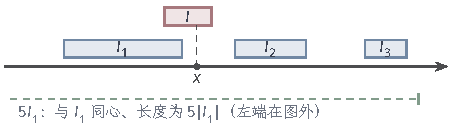
\includegraphics[width=76.616mm]{figures/02-abstract-mathematics/01-metric-and-measure/tikz/c3-vitali-cover/figure.pdf}
\caption{Vitali选择中的五倍放大。蓝色为已选的两两不交区间$I_1=[0.5,2.5]$、$I_2=[3.4,4.6]$、$I_3=[5.6,6.3]$；红色区间$I=[2.2,3.0]$含点$x$，与$I_1$相交且$|I|=0.8<2|I_1|$，因此落在与$I_1$同心、长为$5|I_1|=10$的区间$5I_1=[-3.5,6.5]$中（绿色虚线只画出右侧部分）。}
\label{fig:integral-vitali-cover}
\end{figure}

为描述导数可能不存在的情况，对$x\in(a,b)$引入四个\term{Dini导数}（Dini derivative）：
\[
 \begin{gathered}
 D^+F(x)=\limsup_{h\downarrow0}\frac{F(x+h)-F(x)}h,\\
 D_+F(x)=\liminf_{h\downarrow0}\frac{F(x+h)-F(x)}h,
 \end{gathered}
\]
$D^-F(x)$与$D_-F(x)$则分别是左侧差商$\bigl(F(x)-F(x-h)\bigr)/h$在$h\downarrow0$时的上极限与下极限。$F$在$x$处可导当且仅当四者相等且有限。对单调不减的$F$，四者都取值于$[0,\infty]$。

\begin{theorem}[单调函数几乎处处可导]
\label{thm:integral-monotone-differentiable}
设$F:[a,b]\to\mathbb R$单调不减。则$F$在$[a,b]$上几乎处处有有限导数，$F'$（在导数不存在处取$0$）Lebesgue可积，并且
\begin{equation}
 \int_a^bF'(x)\,\mathrm dx\le F(b)-F(a).
 \label{eq:integral-monotone-derivative-bound}
\end{equation}
\end{theorem}

\begin{proof}
先证明四个Dini导数几乎处处相等，这一步是补充阅读，读者可以先接受结论，直接看下一段的积分估计。取有理数$0<u<v$，令$E=\{x\in(a,b):D_-F(x)<u<v<D^+F(x)\}$，$s=\lambda^*(E)$。对$\varepsilon>0$取开集$O\supseteq E$，$\lambda(O)<s+\varepsilon$。每个$x\in E$都有任意小的$h>0$使$[x-h,x]\subseteq O\cap(a,b)$且$F(x)-F(x-h)<uh$；这些区间构成$E$的Vitali覆盖，由引理~\ref{lem:integral-vitali}选出两两不交的$[x_k-h_k,x_k]$（$k\le N$），未覆盖部分外测度小于$\varepsilon$，并且
\[
 \sum_{k=1}^N\bigl(F(x_k)-F(x_k-h_k)\bigr)<u\sum_kh_k\le u\lambda(O)<u(s+\varepsilon).
\]
令$A$为$E$落在这些区间内部的部分，则$\lambda^*(A)>s-\varepsilon$（端点只有有限个）。每个$y\in A$都有任意小的$k>0$，使$[y,y+k]$含于某个$(x_j-h_j,x_j)$且$F(y+k)-F(y)>vk$。再用引理选出两两不交的$J_1,\ldots,J_M$，未覆盖部分外测度小于$\varepsilon$，故$\sum_m|J_m|>s-2\varepsilon$，$F$在这些区间上的增量之和大于$v(s-2\varepsilon)$。每个$J_m$都在某个$[x_k-h_k,x_k]$内，$F$单调不减，同一个$[x_k-h_k,x_k]$内不交子区间上的增量之和不超过它两端的增量。于是$v(s-2\varepsilon)<u(s+\varepsilon)$。令$\varepsilon\to0$得$vs\le us$，而$v>u$，所以$s=0$。对所有有理数对取并，$\{D_-F<D^+F\}$零测，即$D^+F\le D_-F$几乎处处成立。把这一结论用于单调不减函数$\tilde F(x)=-F(-x)$（定义在$[-b,-a]$上），由$D^+\tilde F(x)=D^-F(-x)$、$D_-\tilde F(x)=D_+F(-x)$得到$D^-F\le D_+F$几乎处处成立。于是几乎处处有
\[
 D^+F\le D_-F\le D^-F\le D_+F\le D^+F,
\]
四者相等，$F$的导数在$[0,\infty]$中几乎处处存在。

再证明积分估计，它同时说明导数几乎处处有限。对$x>b$令$F(x)=F(b)$，并令$q_n(x)=n\bigl(F(x+1/n)-F(x)\bigr)$。单调函数的上水平集是区间，所以$F$与$q_n$可测；$q_n\ge0$，并且在导数存在处$q_n\to F'$。由Fatou引理（引理~\ref{lem:integral-fatou}），
\[
 \int_a^bF'\,\mathrm dx\le\liminf_{n\to\infty}\int_a^bq_n\,\mathrm dx.
\]
平移不改变Lebesgue积分（定理~\ref{thm:integral-jacobian-change}，平移的Jacobian因子为$1$），所以
\[
 \begin{aligned}
 \int_a^bq_n\,\mathrm dx&=n\int_{a+1/n}^{b+1/n}F-n\int_a^bF\\
 &=n\int_b^{b+1/n}F-n\int_a^{a+1/n}F\le F(b)-F(a),
 \end{aligned}
\]
最后一步用到$[b,b+1/n]$上$F=F(b)$、$[a,a+1/n]$上$F\ge F(a)$。这就是式~\eqref{eq:integral-monotone-derivative-bound}。左侧有限，可积的非负函数几乎处处有限，所以导数几乎处处有限。
\end{proof}

由$F=V-(V-F)$，有界变差函数是两个单调函数之差，因而也几乎处处可导，并且$|F'|\le V'+(V-F)'$几乎处处成立，导数绝对可积。结合引理~\ref{lem:integral-ac-bv}，绝对连续函数同样几乎处处可导，导数可积。

\paragraph{还没有得到的结论}
式~\eqref{eq:integral-monotone-derivative-bound}只是不等式，等号可以不成立。$[0,1]$上的阶跃函数$F=\mathbf 1_{[1/2,1]}$单调不减，除$x=1/2$外导数都是$0$，导数的积分为$0$，而$F(1)-F(0)=1$；增量全部发生在一个点上，导数读不到它。所以有界变差和导数可积只给出导数的存在与总量的上界，还不能说明导数的积分等于函数的增量。要排除导数读不到的变化，必须用到绝对连续性；在证明之前，不能把待证的微积分基本定理当作依据。

\subsection{积分函数的绝对连续性与导数}
\label{sec:integral-indefinite}

先看微积分基本定理的第一个方向。设$g$在$[a,b]$上Lebesgue可积，令
\[
 G(x)=\int_a^xg(t)\,\mathrm dt\qquad(a\le x\le b),
\]
这里$\int_a^x$表示在$[a,x]$上对$\lambda$积分。我们要证明$G$绝对连续，并且$G'=g$几乎处处成立。

\paragraph{积分函数绝对连续}
多个不交区间上$G$的增量之和不超过$|g|$在这些区间之并上的积分，所以需要的是：测度很小的集合上，$|g|$的积分也很小。

\begin{lemma}[积分的绝对连续性]
\label{lem:integral-small-sets}
设$g$关于$\mu$可积。则对任意$\varepsilon>0$存在$\delta>0$，使对每个满足$\mu(A)<\delta$的可测集$A$，都有$\int_A|g|\,\mathrm d\mu<\varepsilon$。
\end{lemma}

\begin{proof}
把$|g|$分成有界的截断$\min(|g|,n)$与尾部$|g|-\min(|g|,n)$。截断随$n$递增到$|g|$，单调收敛定理给出$\int\min(|g|,n)\,\mathrm d\mu\uparrow\int|g|\,\mathrm d\mu<\infty$，所以可取$n$使尾部的积分小于$\varepsilon/2$。令$\delta=\varepsilon/(2n)$。当$\mu(A)<\delta$时，
\[
 \int_A|g|\,\mathrm d\mu\le\int_A\min(|g|,n)\,\mathrm d\mu+\int\bigl(|g|-\min(|g|,n)\bigr)\,\mathrm d\mu<n\delta+\frac\varepsilon2=\varepsilon.
\]
\end{proof}

对$[a,b]$中两两不交的$(a_i,b_i)$，令$A=\bigcup_i(a_i,b_i)$，则
\[
 \sum_i|G(b_i)-G(a_i)|=\sum_i\Bigl|\int_{a_i}^{b_i}g\Bigr|\le\int_A|g|\,\mathrm d\lambda.
\]
总长$\lambda(A)<\delta$时右侧小于$\varepsilon$，所以$G$绝对连续。例如在$[0,4]$上取$g(t)=1/(2\sqrt t)$，它在原点附近无界，但$\int_0^4g=2$有限；$G(x)=\int_0^xg=\sqrt x$（对$[\eta,x]$用卷一的公式再令$\eta\downarrow0$，由单调收敛得到），因此$\sqrt x$绝对连续，这正是图~\ref{fig:integral-absolute-continuity-intervals}中的函数。

\paragraph{Lebesgue微分定理}
$G$绝对连续，由上一小节它几乎处处可导；剩下的问题是导数是否等于$g$。卷一的结论只在$g$的连续点处成立，而可积函数可以处处不连续，例如$[0,1]$上有理数的示性函数，它的积分函数恒为$0$，导数$0$与原函数只在零测的有理点上不同。下面的定理说明，“几乎处处”正是一般情形下的准确答案。

\begin{lemma}[区间积分全为零的函数]
\label{lem:integral-vanishing-intervals}
设$g$在$[a,b]$上可积且为实值。若对每个$x\in[a,b]$都有$\int_a^xg=0$，则$g=0$几乎处处成立。
\end{lemma}

\begin{proof}
改动零测集不影响结论，不妨设$g$是Borel函数。令$\mathcal D$为使$\int_Eg=0$的Borel集$E\subseteq[a,b]$全体。区间$(c,d]\subseteq[a,b]$满足$\int_{(c,d]}g=\int_a^dg-\int_a^cg=0$，这些区间和空集对有限交封闭，生成$[a,b]$上的Borel $\sigma$代数（单点也是零测的，可以并入）。$\mathcal D$是$\lambda$系统：$[a,b]\in\mathcal D$；补集由$\int_{E^c}g=\int g-\int_Eg$得到；两两不交的可数并由控制收敛定理（以$|g|$为控制）得到积分可数可加。由$\pi$--$\lambda$定理，$\mathcal D$包含全部Borel集。取$E=\{g>0\}$，得$\int g\mathbf 1_{\{g>0\}}=0$，非负函数积分为零，所以$g\le0$几乎处处成立；同理$g\ge0$几乎处处成立。
\end{proof}

\begin{theorem}[Lebesgue微分定理]
\label{thm:integral-lebesgue-differentiation}
设$g$在$[a,b]$上Lebesgue可积，$G(x)=\int_a^xg(t)\,\mathrm dt$。则$G$绝对连续，并且$G'=g$几乎处处成立，即对几乎每个$x\in(a,b)$，
\[
 \lim_{h\to0}\frac1h\int_x^{x+h}g(t)\,\mathrm dt=g(x).
\]
\end{theorem}

\begin{proof}
绝对连续性已经证明。复值情形对实部、虚部分别处理，实值情形由$g=g^+-g^-$与导数的线性性，只需对$g\ge0$证明。

先设$0\le g\le M$。此时$|G(y)-G(x)|\le M|y-x|$，$G$是Lipschitz函数，由上一小节它几乎处处可导。对$x>b$令$G(x)=G(b)$，差商$q_n(x)=n\bigl(G(x+1/n)-G(x)\bigr)$满足$|q_n|\le M$，并在$G$可导的点趋于$G'$。对$c\in(a,b]$，在$[a,c]$上以常数$M$为控制用控制收敛定理，再像定理~\ref{thm:integral-monotone-differentiable}的证明那样平移，得
\[
 \int_a^cG'\,\mathrm dx=\lim_{n\to\infty}\Bigl(n\int_c^{c+1/n}G-n\int_a^{a+1/n}G\Bigr)=G(c)-G(a),
\]
最后一步用到$G$连续，函数在缩小区间上的平均值趋于端点值。于是$\int_a^c(G'-g)=0$对所有$c$成立，由引理~\ref{lem:integral-vanishing-intervals}，$G'=g$几乎处处成立。

再看一般的$g\ge0$。令$g_n=\min(g,n)$，$G_n(x)=\int_a^xg_n$。由有界情形，$G_n'=g_n$几乎处处成立。$G-G_n=\int_a^x(g-g_n)$单调不减，其导数在几乎每点非负，所以$G'\ge G_n'=g_n$几乎处处成立；对可数个$n$合并例外集，得$G'\ge g$几乎处处成立。另一方面，$G$单调不减，由式~\eqref{eq:integral-monotone-derivative-bound}，
\[
 \int_a^bG'\le G(b)-G(a)=\int_a^bg.
\]
因此$G'-g\ge0$几乎处处成立且积分不超过$0$，故$G'=g$几乎处处成立。最后，$G'(x)=g(x)$按定义就是$\frac1h\bigl(G(x+h)-G(x)\bigr)=\frac1h\int_x^{x+h}g\to g(x)$。
\end{proof}

\term{Lebesgue微分定理}的名称来自最后一种表述：$g$在$x$附近的局部平均值，在几乎每一点恢复$g$的取值。常见的另一种证明先建立最大平均值函数的弱型估计，再用连续函数逼近可积函数；这里改用单调函数的可导性和上面的区间引理，二者都是一元区间上的论证，不需要后面的函数空间完备性，也不使用第四章的相对密度定理。

\subsection{微积分基本定理}
\label{sec:integral-ftc}

现在处理第二个方向：给定绝对连续的$F$，证明$F(x)-F(a)=\int_a^xF'$。由第~\ref{sec:integral-bounded-variation}小节，$F'$几乎处处存在且可积；令$G(x)=F(a)+\int_a^xF'(t)\,\mathrm dt$。由上一小节，$G$绝对连续且$G'=F'$几乎处处成立。于是$H=F-G$绝对连续，并且$H'=0$几乎处处成立。恢复公式就归结为：导数几乎处处为零的绝对连续函数必为常数。

\paragraph{零导数引理}
阶跃函数和Cantor函数说明，没有绝对连续性时这个结论不成立。绝对连续性的作用，是控制导数为零的点之外那些总长很小的间隙上的增量。

\begin{lemma}[零导数引理]
\label{lem:integral-zero-derivative}
若$H$在$[a,b]$上绝对连续，且$H'=0$几乎处处成立，则$H$是常数。
\end{lemma}

\begin{proof}
任取$c\in(a,b]$，证明$H(c)=H(a)$。给定$\varepsilon>0$，取绝对连续定义中的$\delta$。令$E=\{x\in(a,c):H'(x)=0\}$，则$\lambda(E)=c-a$。对每个$x\in E$，$H'(x)=0$保证有任意小的$h>0$，使$[x,x+h]\subseteq(a,c)$且$|H(x+h)-H(x)|<\varepsilon h$。这些区间构成$E$的Vitali覆盖。由引理~\ref{lem:integral-vitali}，可以选出两两不交的$[x_k,y_k]$（$k=1,\ldots,N$，按$x_1<y_1<x_2<\cdots<y_N$排列），使$\lambda\bigl(E\setminus\bigcup_k[x_k,y_k]\bigr)<\delta$。

记$y_0=a$、$x_{N+1}=c$。$[a,c]$去掉所选区间后剩下的间隙$(y_k,x_{k+1})$（$k=0,\ldots,N$）两两不交，总长不超过$\lambda\bigl(E\setminus\bigcup_k[x_k,y_k]\bigr)+\lambda([a,c]\setminus E)<\delta$。把端点增量沿选中区间和间隙拆开：
\[
 \begin{aligned}
 |H(c)-H(a)|&\le\sum_{k=1}^N|H(y_k)-H(x_k)|+\sum_{k=0}^N|H(x_{k+1})-H(y_k)|\\
 &<\varepsilon\sum_k(y_k-x_k)+\varepsilon\le\varepsilon(c-a+1).
 \end{aligned}
\]
前一项由导数为零控制，后一项由绝对连续性控制。$\varepsilon$任意，所以$H(c)=H(a)$。
\end{proof}

\paragraph{恢复公式与双向刻画}
零导数引理补上了最后一步。

\begin{theorem}[Lebesgue微积分基本定理]
\label{thm:integral-ftc}
设$F:[a,b]\to\mathbb R$。以下两条等价：
\begin{enumerate}
 \item $F$在$[a,b]$上绝对连续；
 \item 存在$[a,b]$上的Lebesgue可积函数$g$，使$F(x)=F(a)+\int_a^xg(t)\,\mathrm dt$对所有$x\in[a,b]$成立。
\end{enumerate}
此时$F$几乎处处可导，$F'=g$几乎处处成立，并且
\begin{equation}
 F(x)-F(a)=\int_a^xF'(t)\,\mathrm dt\qquad(a\le x\le b).
 \label{eq:integral-ftc}
\end{equation}
\end{theorem}

\begin{proof}
(2)推出(1)及$F'=g$几乎处处成立，就是定理~\ref{thm:integral-lebesgue-differentiation}。(1)推出(2)：如本小节开头所述，$F'$几乎处处存在且可积，$H=F-F(a)-\int_a^xF'$绝对连续且$H'=0$几乎处处成立，由引理~\ref{lem:integral-zero-derivative}，$H$恒等于$H(a)=0$，这就是式~\eqref{eq:integral-ftc}，取$g=F'$即得(2)。
\end{proof}

\term{微积分基本定理}的这一形式给出了双向刻画：绝对连续函数恰好是可积函数的不定积分加上常数，并且这个可积函数在几乎处处的意义下唯一确定为$F'$。连续可导函数与Lipschitz函数都绝对连续，因而都满足式~\eqref{eq:integral-ftc}；Lipschitz函数可以在零测集上不可导，例如$|x|$，但这不影响恢复公式。

\paragraph{分部积分}
恢复公式使一元\term{分部积分}（integration by parts）推广到绝对连续函数。

\begin{theorem}[绝对连续函数的分部积分]
\label{thm:integral-integration-by-parts}
若$F,G$在$[a,b]$上绝对连续，则$FG$绝对连续，$F'G$与$FG'$可积，并且
\[
 \int_a^bF'(x)G(x)\,\mathrm dx=F(b)G(b)-F(a)G(a)-\int_a^bF(x)G'(x)\,\mathrm dx.
\]
\end{theorem}

\begin{proof}
$F,G$在紧区间上连续，取$M$使$|F|,|G|\le M$。对每个区间，
\[
 |F(b_i)G(b_i)-F(a_i)G(a_i)|\le M|G(b_i)-G(a_i)|+M|F(b_i)-F(a_i)|,
\]
所以$FG$的总增量受$F,G$总增量的$M$倍控制，$FG$绝对连续。在$F,G$都可导的点（几乎处处）有$(FG)'=F'G+FG'$；$F'$可积而$G$有界，所以$F'G$可积，$FG'$同理。对$FG$用式~\eqref{eq:integral-ftc}，再由积分的线性性移项即得。
\end{proof}

例如在$[0,1]$上取$F(x)=\sqrt x$、$G(x)=x$。$F'=1/(2\sqrt x)$在原点附近无界，经典公式要求的连续导数不存在，但定理仍适用：$\int_0^1\frac{x}{2\sqrt x}\,\mathrm dx=\frac13$，右侧为$1\cdot1-0-\int_0^1\sqrt x\,\mathrm dx=1-\frac23=\frac13$，两侧一致。

\subsection{Cantor函数与恢复公式的边界}
\label{sec:integral-cantor-boundary}

第~\ref{sec:measure-decomposition}节已经构造了Cantor函数，这里记为$c:[0,1]\to[0,1]$，只用它检验恢复公式，不再重复构造。它的性质是：连续、单调不减，$c(0)=0$、$c(1)=1$；在构造Cantor集时删去的每个开区间上取常值；构造的第$n$步有$2^n$个保留的闭区间，每个长$3^{-n}$，$c$在每个保留区间上恰好增加$2^{-n}$。图~\ref{fig:integral-cantor-function}(a)画出了前几步的分段线性逼近，(b)标出了第二步的四个保留区间。

\begin{figure}[!htbp]
\centering
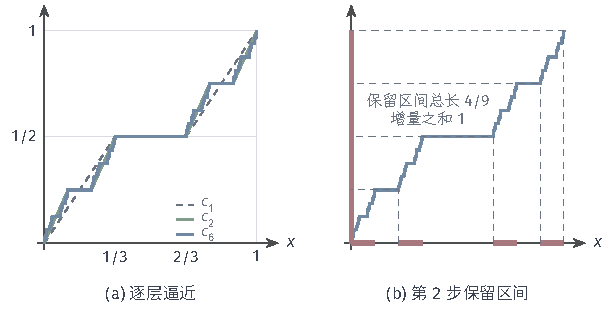
\includegraphics[width=103.847mm]{figures/02-abstract-mathematics/01-metric-and-measure/tikz/c3-cantor-function/figure.pdf}
\caption{Cantor函数及其分段线性逼近。(a)$c_1$（虚线）、$c_2$（绿色）与$c_6$（蓝色），$c_n$在第$n$步的$2^n$个保留区间上线性增加$2^{-n}$，在已删去的区间上保持常值；(b)第二步的四个保留区间$[0,\frac19]$、$[\frac29,\frac13]$、$[\frac23,\frac79]$、$[\frac89,1]$（横轴红色）总长$4/9$，对应的增量（纵轴红色）各为$1/4$，合起来覆盖整个$[0,1]$。}
\label{fig:integral-cantor-function}
\end{figure}

\paragraph{导数读不到的增量}
Cantor集$C$的补集是删去的开区间之并，$c$在其中每个开区间上为常值，所以在$[0,1]\setminus C$的每一点导数为$0$。第二章已经证明$\lambda(C)=0$，因此$c'=0$几乎处处成立，而
\[
 \int_0^1c'(x)\,\mathrm dx=0\ne1=c(1)-c(0).
\]
恢复公式~\eqref{eq:integral-ftc}失败。由定理~\ref{thm:integral-ftc}，$c$不可能绝对连续。这一点也可以直接从定义看出：第$n$步的$2^n$个保留区间（取其内部）两两不交，总长$(2/3)^n\to0$，而$c$在它们上的增量之和始终是$2^n\cdot2^{-n}=1$。所以对$\varepsilon=1$，任何$\delta>0$都会被足够大的$n$打破。

\paragraph{几种性质的比较}
Cantor函数把几种容易混淆的性质分开了。它连续，所以连续不能保证恢复公式；它单调，因而有界变差，并且几乎处处可导，所以这两条也不够；它缺的正是绝对连续性。前面的例子还给出另一侧的分界：$x\sin(1/x)$一致连续却不是有界变差；$\sqrt x$绝对连续却不Lipschitz。概括起来，在$[a,b]$上
\[
 \text{Lipschitz}\Longrightarrow\text{绝对连续}\Longrightarrow\text{连续且有界变差}\Longrightarrow\text{几乎处处可导},
\]
而三个箭头都不能反过来，反例依次是$\sqrt x$、Cantor函数和阶跃函数$\mathbf 1_{[1/2,1]}$（几乎处处可导但不连续）。

Cantor函数那部分导数读不到的增量，正是第二章的奇异连续质量：它没有点质量，却全部集中在零测的Cantor集上（第~\ref{sec:measure-decomposition}节）。一般的有界变差函数，其增量可以分成由导数积分恢复的部分、跳跃部分和这种奇异连续部分；第四章将把函数增量看作测度，用相对于Lebesgue测度的密度重新解释本节的结论。

\section{本章小结}
\label{sec:integral-summary}

本章回答的问题是：给定测度，怎样累计一个函数的取值，以及累计之后哪些运算可以交换。积分从简单函数的分块累计开始（第~\ref{sec:integral-definition}节）：在取值固定的可测块上，贡献就是取值乘以块的测度。非负可测函数用下方简单函数的积分上确界定义，二进制分层逼近说明这个上确界确实能逐层读出函数；可正可负的函数拆成正部和负部，复值函数拆成实部和虚部，绝对可积条件保证不出现$\infty-\infty$；对有符号测度则沿Jordan分解分别积分。整个构造只用到测度和被积函数本身，不需要先寻找哪个测度的密度。随后，单调收敛定理把简单函数的运算规则传递到一般函数（第~\ref{sec:integral-properties}节），离散求和、闭区间上的Riemann积分和绝对收敛的反常积分都成为同一积分的特例（第~\ref{sec:integral-classical}节）。

本章的大部分结论都在回答“什么条件允许交换两种运算”，而起作用的条件可以按运算归纳为表~\ref{tab:integral-summary-conditions}。非负性和单调递增支持递增累计，结果允许为无穷；共同的可积控制防止质量逃逸，支持极限与积分交换（第~\ref{sec:integral-limits}节）；绝对可积性防止正负贡献以不同方式抵消，支持改变累次积分的次序（第~\ref{sec:integral-iterated}节）。换元则按映射的条件逐层具体化：一般可测映射只需推前测度，可逆光滑变换由Jacobian行列式给出体积比例，分支可逆变换要累计所有原像分支（第~\ref{sec:integral-change-of-variables}节）。含参积分把参数变化转成函数列的极限，连续性与积分号下求导都要求在参数点附近有统一的可积控制（第~\ref{sec:integral-parametric}节）。

\begin{table}[!htbp]
\centering
\caption{本章主要运算及其成立条件。非负情形的等式允许两侧同为$+\infty$；表中条件都是充分条件，反例说明去掉条件后结论可能失败。}
\label{tab:integral-summary-conditions}
\small
\begin{tabularx}{\linewidth}{@{}l>{\RaggedRight\arraybackslash}X>{\RaggedRight\arraybackslash}X@{}}
\toprule
运算 & 条件 & 依据与反例\\
\midrule
极限与积分交换 & 非负递增 & 单调收敛\\
 & 几乎处处收敛，有可积控制 & 控制收敛；$n\mathbf 1_{(0,1/n)}$\\
累次积分换序 & 非负，两侧$\sigma$有限 & Tonelli；对角线反例\\
 & 乘积测度下绝对可积 & Fubini；有理函数反例\\
换元 & 可测映射 & 推前换元\\
 & 微分同胚或可数分支 & Jacobian公式；分支累计\\
参数连续、求导 & 参数点附近统一控制 & 控制收敛；$te^{-tx}$\\
由导数恢复函数 & 绝对连续 & 基本定理；Cantor函数\\
\bottomrule
\end{tabularx}
\end{table}

积分与微分的关系在第~\ref{sec:integral-differentiation}节收束。可积函数的不定积分绝对连续，并且在几乎每一点的导数等于原函数；反过来，绝对连续函数恰好是其导数的不定积分加常数。两个方向分别依靠积分在小测度集上的绝对连续性、单调函数的几乎处处可导，以及区间覆盖下的零导数引理。导数可积与能够由导数恢复函数是两回事：阶跃函数和Cantor函数都几乎处处可导、导数可积，却不能由导数恢复；后者连续单调，增量全部落在零测的Cantor集上。

下一章把问题反过来。本章固定一个测度，用函数的积分产生数值；如果给定两个测度，能否找到一个函数，使它相对于参考测度的积分恢复目标测度在每个集合上的质量？Cantor函数已经显示这样的函数未必存在。第四章将以本章的积分定义、单调收敛定理和基本运算为依据，研究这种密度何时存在、怎样计算，以及如何用它在同一空间上转换积分。

